\chapter{Introduction}\label{intro}
 \section{Elementary modes of excitation}
Subject to external probes which couple weakly to the nucleus, that is in such a way that the system can be expressed in terms of the properties of the excitation in the absence of probes\footnote{\cite{Pines:66},\cite{Bohr:75}} , the nucleus reacts  in terms  of single--particle (--hole) motion (one--particle transfer), vibrations (surface, spin, etc.) and rotations (Coulomb excitation and inelastic scattering) and pairing vibrations and rotations (two--nucleon transfer reactions) (see Figs. \ref{figintro1}, \ref{figintro2} and \ref{figintro3}, also Sect. \ref{C1S7.1}).

\begin{figure}
\centerline {
\includegraphics*[width=15cm]{introduccion/figs/figintro1}
}
\caption{Schematic representation of: \textbf{a}) \textbf{elastic} (population of the ground state), and \textbf{inelastic} \textbf{b}) (population lowest octupole vibration 2.62 MeV) processes associated with the reaction $^{208}$Pb$(\alpha,\alpha')^{208}$Pb (for more details see Sect. \ref{appintroD}). In the inset (II) one of the NFT(r+s) diagrams describing the  excitation of the low--lying octupole vibration (wavy line), of $^{208}$Pb  is given. A pointed (curved) arrow on a line indicates propagation of a nucleon in the target nucleus (in the continuum). The horizontal dashed line represents the action of the mean field (see Fig. \ref{figintro4}) while the solid dot stands for the particle--vibration coupling vertex (Sect. \ref{appintroD}). In the inset (I) a NFT(r+s) diagram describing  the elastic process (potential scattering) is displayed. From the measurement of the differential cross section one can deduce the partial wave phase shifts (Appendix \ref{App1.D}) Outgoing particles are deflected in a spectograph and recorded in a detector. The corresponding excitation function is given in the lowest part of the figure (after \cite{Mottelson:76b}).}
\label{figintro1}
\end{figure}
\begin{figure}
\centerline {
\includegraphics*[width=12cm]{introduccion/figs/figintro2}
}
\caption{Schematic cartoon representation of the one--nucleon transfer reaction $^{208}$Pb$(d,p)^{209}$Pb populating the single--particle states of $^{209}$Pb. In the inset a NFT(r+s) diagram describing the process is shown. A standard (pointed) arrowed curve indicates the transferred nucleon, moving with the proton in the deuteron (double, curve arrowed, line), or around the (assumed, for simplicity, inert) $^{208}$Pb core. The energy of the outgoing proton reflects both the $Q$--value of the reaction and the excitation energy of the final state. In the inset, a NFT(r+s) diagram describing one of the possible transfer  processes is schematically shown. An arrowed curve indicates the transferred nucleon. The jagged curve represents the recoil elementary mode which couples (dashed square) the relative motion (reaction) to the intrinsic nucleonic degrees of freedom  (structure) through a Galilean operator transformation. For more details see caption to Fig. \ref{figintro1} and \ref{fig1.9.2}, see also Ch. \ref{C6} and Fig. \ref{fig6.1.1} as well as App. \ref{App1.D} and Sect. \ref{C7AppC} (after \cite{Mottelson:76b}).}
\label{figintro2}
\end{figure}
\begin{figure}
\centerline {
\includegraphics*[width=9cm]{introduccion/figs/figintro3}
}
\caption{Schematic representation of the two--nucleon transfer reaction $^{208}$Pb$(t,p)^{210}$Pb populating the ground state $0^+$, and two particle excited states $2^+$ and $4^+$ (monopole, quadrupole and hexadecapole pair addition modes of $^{208}$Pb, i.e. multipole pariring vibrations, see \cite{Brink:05} Sect. 5.3.1 p. 108, \cite{Broglia:74}, \cite{Ragnarsson:76}, \cite{Broglia:71b}, \cite{Broglia:71c}, \cite{Bes:71d}, \cite{Bes:71}, \cite{Flynn:71}, \cite{Bes:72}, \cite{Broglia:81c}, \cite{Bohr:74b}, \cite{Flynn:72}, \cite{Bortignon:76}; see also \cite{Kubo:70}). In the inset a NFT(r+s) diagram of the transfer process is displayed. In selecting it, it was  assumed, as detailed calculations indicate, that the main contribution to the process arises from the successive transfer of the nucleons. The jagged curves represent the recoil  mode coupling the intrinsic and the relative motion,  thus accounting for the mass partition associated with the different channels and the change in scaling between entrance and exit channel distorted waves. The corresponding momentum mismatch being taken care by Galilean transformations (recoil effects) (see also caption to Fig. \ref{figintro2} and App. \ref{App1.D}; also Ch. \ref{C7}, in particular Figs. \ref{figC7C1} and \ref{figC7C2}). As discussed in the following Chapters (see in particular Chs. \ref{chapter1} and \ref{chapter2}), Cooper pairs are extended objects, the fermionic partners being correlated over distances much larger than nuclear dimensions (correlation length $\xi\approx36$ fm$\gg 2R_0\approx 14.2$ fm ($A=208$)). Because the single particle potential acts on these pairs as a rather strong external field, this feature is not obvious in structure calculations, becoming apparent in reaction calculations. The dineutron moving in the triton and around the $^{208}$Pb, (assumed for simplicity to be inert) is represented by a double arrowed line. Each individual transferred neutron is indicated with a single arrowed line. The curved arrows on the triton and on the proton indicate motion in the continuum with outgoing and incoming asymptotic waves, respectively. The arrow encompassing the pair addition mode and the core $^{208}$Pb, indicate intrinsic (structure) motion (after \cite{Mottelson:76b}).}
\label{figintro3}
\end{figure}

In the figures, a cartoon representation (color online) of elastic, inelastic, one-- and two--particle direct transfer reactions induced by alpha and proton projectiles impinging on $^{208}$Pb are shown. In all cases a standard setup is used, in which a light projectile is aimed at a fixed target (thin foil made out of $^{208}$Pb). The outgoing particles carrying the corresponding physical information, i.e. momentum, angular momentum, energy, etc. transferred to or from the target, are deflected by the electromagnetic fields of a spectrometer and eventually recorded at a given angle by particle detectors (points a,b\dots in magnet). Those events provide structural information as shown in the two dimensional strength function displayed below the cartoon laboratory setup. 

These strength functions, recorded at a wide range of angles provide the absolute differential cross sections of each of the nuclear states populated in the process. They are  typically measured in millibarns per  steradian (mb/sr). To translate these quantities into nuclear structure information, a model of structure and of reactions is needed to calculate the absolute cross sections, to be compared with the data. The risks of using relative cross section is that of overlooking limitations in the description of the reaction mechanism or in that of the structure description of the states involved in the reaction under study. Or of both.

In this connection, it is of notice that either one sets equal weight in correctly calculating the mean field properties and the clothing of the single--particles (i.e. the physical nucleons (structure, see e.g. Figs. \ref{figintro4} and \ref{fig:4.2})) than in working out the reaction mechanism (see Ch. \ref{C6}), or the confrontation between theoretical predictions and experimental observation would unlikely be fruitful\footnote{\textit{Structure and Reactions}. Within this context one can ask how one understands what the correct elements are to describe a reaction process, if one does not know in detail the structure of the initial and final states? In a nutshell: how can one understand reaction without knowing structure (eyes without object)?. 


Vice versa, how can one understand what the elements needed for a correct description of the structure of levels is, if one does not know how to observe them, how to bring that information to the detector?. In other words, how can one understand structure without knowing reaction (object without eyes)? The answer to both questions is that you cannot. As simple as that.}. Arguably, an example of such an approach is given in Sect. \ref{C1S10} of this Chapter.


Echoing Heisenberg's requirement \footnote{\cite{Heisenberg:49}.} that no concept enters the quantal description of a physical system which has no direct relation to experiments, and Landau's result that any weakly excited state of a quantal many--body system may be regarded as a gas of weakly interacting elementary modes of excitation\footnote{\cite{Landau:41}).}, Bohr, Mottelson and coworkers\footnote{\cite{Bohr:69}, \cite{Bohr:76}, \cite{Mottelson:76}, \cite{Bohr:75}, \cite{Bohr:58}, \cite{Belyaev:59}, \cite{Nilsson:55},  \cite{Bes:66}.} developed a unified field theoretical description of the nuclear  structure (Nuclear Field Theory, NFT) in terms of quasiparticles, vibrations and rotations, both in 3D-- as well as in gauge-- and other ``abstract'' spaces, with close connections with direct nuclear reactions\footnote{ \cite{Alder:56}, \cite{Alder:75}, \cite{Broglia:04a}, \cite{Austern:70}, \cite{Glendenning:04}, \cite{Satchler:80}, \cite{Satchler:83}, see also \cite{Potel:13}.}. Within this context also given in Figs. \ref{figintro1}--\ref{figintro3} (insets) are \textit{unified NFT diagrams of structure and reactions (NFT(s+r))}\footnote{ \cite{Broglia:79b,Broglia:04a,Broglia:16}}, which microscopically describe the variety of processes in terms of elementary modes of excitation. That is, in the present case in which the target is a closed shell system, a particle--hole (inelastic scattering), one--particle (single--particle stripping) and two--particle (Cooper pair transfer) modes.

In keeping with the fact that all the nuclear degrees of freedom are exhausted by those of the nucleons, and that the different reactions, that is Coulomb, inelastic and one-- and two-- particle transfer reactions project particular, but somewhat
 overlapping  components of the total wavefunction, the nuclear elementary modes of excitation give  rise to an overcomplete, non orthogonal, Pauli principle violating basis, both concerning structure as well as reactions. The coupling between unperturbed fermionic and bosonic degrees of freedom is proportional to this overlap between single--particle and collective modes. Nuclear Field Theory\footnote{\cite{Bes:76a}, \cite{Bes:76b}, \cite{Bes:76c}, \cite{Bes:75}, \cite{Broglia:76}, \cite{Bes:75b}, \cite{Mottelson:76}, \cite{Bes:77}, \cite{Bortignon:77}, \cite{Bortignon:78}, \cite{Broglia:04a},\cite{Reinhardt:75},\cite{Reinhardt:78a},\cite{Reinhardt:78b},\cite{Reinhardt:80}.}, provides the conserving sum rules protocol to diagonalize these couplings  to any order of perturbation theory, also infinite if so required for specific processes. The clothed physical elementary modes resulting from the interweaving of the bare modes are orthogonal to each other, fulfill Pauli principle, and behave like a non interacting gas, providing a microscopic solution to the many--body nuclear problem. Its predictions, embodied in absolute cross sections and transition probabilities, can be directly compared with the observables whose values are obtained by studying the nuclear system with  the variety of ever more precise and varied arsenal of experimental probes\footnote{\label{foot1}What NFT cannot do, is to solve problems regarding ill behaved bare forces, or the consequences of associated particle--vibration coupling vertices which eventually lead to divergences. Within this context, \textit{empirical renormalization} has proved to be a powerful and physically consistent prescription to implement the NFT and to make connection with experimental data (see e.g. Sect. \ref{C6S2}, see also \cite{Barranco:04} and \cite{Broglia:16}, and refs. therein)}.

At this point a proviso or two are in place. The original elementary modes of nuclear excitation melt together, due to their interweaving, into effective fields. Each of them display properties which reflects that of all the others, their individuality resulting from the actual relative importance of each one of them. What one calls physically a (clothed) particle is only partially to be associated with that particle field alone. It is also partially to be associated with the  vibrational fields (surface, density, spin, pairing, etc.), because they are in interaction through the particle--vibration coupling vertices. And conversely, what one calls a nuclear vibration can couple to  particle--hole (in the case of a surface vibration),  two--particle (in the case of a pair addition) or a two--hole (in the case of a pair removal)  configurations. The associated fermions  can   couple to other vibrational modes and, eventually   in the course of time, recombine to reform the original vibration. The outcome of such processes, namely the dressed physical elementary modes of excitation, is closely connected with the renormalization program of quantum electrodynamics (QED)\footnote{\cite{Schwinger:01}.} implemented, in NFT, in terms of Feynman diagrams\footnote{\cite{Feynman:75}.} and made operative in a number of cases in term of empirical renormalization prescription\footnotemark[\ref{foot1}]. The specific experimental probes of the bare elementary modes of nuclear excitation reveal only one, in most cases likely the most important aspects of the physical (clothed) elementary modes. Renormalization (NFT program) reflects the physical unity of  low--energy nuclear research requiring the melting not only of elementary modes of excitation but also of structure and reaction theory, let alone of the different experimental techniques developed to study the atomic nucleus (Within this context cf. Ch.  Fig. \ref{fig1.4.1}). 


As can be seen from the contents of the present monograph, the accent is set on relating theoretical prediction with experimental finding, through the unification of structure and reactions. In particular the unification of pairing and two--nucleon transfer, where the two subjects are blended together, which is what happens in nature.
The theory of direct reaction for two--particle transfer is discussed in Ch. \ref{C7} (see summary Sect. \ref{C7S1}). To be operative, two--nucleon spectroscopic amplitudes and optical potentials are needed. One--particle transfer processes are at the basis of the above derivations, and are summarized in Sect. \ref{C4S1}. Once the NFT rules to work the variety of elements (spectroscopic and, with the help of them, reaction amplitudes) have been laid  out and/or the pertinent literature refer to, concrete embodiments are provided and eventual absolute cross sections calculated and confronted with the experimental data (for details see App. \ref{appintroAx}). Within this scenario, once the NFT renormalization program associated with a characterising set of observables, e.g. the energy ($\hbar \omega_{2^+}$) and electromagnetic transition probability ($B(E2)$) of the collective, low--lying quadrupole vibration of $^{120}$Sn has been carried out, a decision is to be taken. Unless one is not specifically studying such type of nuclear excitations, e.g. through inelastic scattering, but just using them to e.g. cloth single--particles, one turns to the \textit{empirical renormalization} program\footnote{\cite{Barranco:01,Idini:14,Idini:15,Broglia:16}}. Within the framework of the particular example, one calculates the $\hbar \omega_{2^+}$ and $B(E2)$ values making use of the harmonic approximation to diagonalize  a separable quadrupole--quadrupole interaction adjusting its strength $k_2$ so as to reproduce the experimental findings. As a rule, the resulting $k_2$ has a value close to that required by self consistency\footnote{\cite{Bohr:75}} (see also Sect. \ref{appintroD}). Within the properties mentioned, i.e. single--particle self energy, the final outcome differs little from  that obtained from a full implementation of the NFT renormalization program. On the other hand, the use of the \textit{empirical renormalization} program, aside from being an economic procedure for self consistency in phonon renormalization, allows to avoid difficulties associated with the zero--range character (ultraviolet divergences) and finite size instabilities of many effective  interactions.


%\begin{align}
%\ket{\widetilde {sp}}=\alpha\ket{sp}+\beta\ket{(sp)'\otimes \lambda}\\
%x=\frac{G2\Omega}{D}=GN(0)\\
%\tilde x =\tilde G \tilde N(0)\\
%\tilde G=Z^2(G+G_{ind})\\
%\tilde N(0)=N(0)/Z\\
%\tilde x=Z(G+G_{ind})N(0)
%\end{align}





\section{Sum rules}
A quantitative measure of the overcompleteness mentioned above and concerning the elementary modes of excitation basis is provided by the use of exact and approximate sum rules that the observables (cross sections) associated with the variety of probes to which the nucleus is subject, have to fulfill. An example of the first type (exact) is provided by the Thomas--Reiche--Kuhn (TRK) sum rule. Of the second type (approximate) by some of the two--nucleon transfer (TNTR) sum rules\footnote{\cite{Broglia:72b}}. Others, which relate one-- with two--particle transfer processes\footnote{\cite{Bayman:72,Lanford:77}} being exact. In both cases they embody particle (pair) number conservation. Charged particles in the first case (electrons in atoms and molecules, effective charges of neutrons and protons in nuclei). Number of Cooper pairs in nuclei in the second. Physically, they provide  information concerning: 1) the maximum amount of energy which the quantal system can absorb from a beam of light ($\gamma$--rays) shined on it; 2) the total two--nucleon transfer cross section (ring area fraction of the total (geometrical) reaction cross section) exhausted by the final ($A\pm2$) states populated in the transfer process.


In other words, these sum rules provide: a quantitative measure of the single--particle subspace the quantal system under study, in particular the nucleus, uses to correlate particle--hole excitations and thus induce the antenna--like motion of protons against neutrons or, to correlate pairs of nucleons moving in time reversal states around the Fermi energy, leading to a sigmoidal distribution of the associated level occupancy\footnote{Within this context, the absolute two--nucleon transfer cross section populating the ground state of a superfluid nucleus is proportional to the number of Cooper pairs contributing to the nuclear condensate. This quantity is rather stable along a pairing rotational band, in keeping with the fact that the ``intrinsic'' $|BCS\rangle$--state of the deformed system in gauge space, is essentially the same for all members of the band. This fact is at the basis of an approximate, physically sum rule.}. 


The TRK sum rule can, in the nuclear case, be written as\footnote{\cite{Bohr:75,Bertsch:05,Bortignon:98}}
\begin{align}\label{eq_intro1}
S(E1)=\sum_\alpha\left|\langle\alpha|F|\tilde 0\rangle\right|^2(E_\alpha-E_0)=\frac{9}{4\pi}\frac{\hbar^2e^2}{2m}\frac{NZ}{A},
\end{align}
where $|\alpha\rangle$ labels the complete set of excited dipole states which can be reached operating with the dipole operator $F$ on the initial correlated vacuum state $|\tilde 0\rangle$. Within this context, each elementary mode of excitation, provides a specific contribution to the total zero point fluctuations of the ground state (ZPF, see Sect. \ref{appintroA}), that is,
\begin{align}\label{eqintro2}
\langle\tilde 0|F^2|\tilde 0\rangle=\frac{\hbar \omega}{2C_\alpha}=\frac{\hbar^2}{2D_\alpha}\frac{1}{\hbar\omega_\alpha}.
\end{align}
In other words, they perturb the static nucleon Fermi sea, that is the set of occupied levels of the mean field potential (Fig. \ref{figintro4})
\begin{align}\label{eqintro3}
U(r)=\int d\mathbf r' \rho(r')v(|\mathbf r-\mathbf r'|),
\end{align}
inducing virtual particle--hole excitations ($k,i$, i.e. $\epsilon_i\leq\epsilon_F$ and $\epsilon_k>\epsilon_F$, see Eqs. (\ref{eqintro6}) and (\ref{eq1.5.1}) (see Fig. \ref{fig1.2.2}). In the above equation, $\rho(r)$ is the nuclear density and $v$ is the nuclear two--body interaction.  


In Eq. (\ref{eq_intro1}), the quantity 
\begin{align}
F=e\sum_n\left(\left(\frac{N-Z}{2A}-t_z(n)\right)r_nY_{1\mu}(\hat r_n)\right),
\end{align}
is the dipole operator acting both on the  protons ($t_z=-1/2$) and on the neutrons ($t_z=1/2$) of mass $m$, as indicated by the $\alpha$--sum over all nucleon states ($A=N+Z$, mass number).

\begin{figure}
\centerline {
\includegraphics*[width=12cm]{introduccion/figs/figintro4}
}
\caption{Schematic representation of the processes characterizing the Hartree--Fock ground state (single--particle vacuum), in terms of Feynman--NFT diagrams. (\textbf{a}) nucleon--nucleon interaction trough the bare (instantaneous) $NN$--potential. (\textbf{b}) Hartree mean field contribution. (\textbf{c}) Fock mean field contribution. (\textbf{d},\textbf{e}) ground state correlations (ZPF) associated with the Hartree and Fock processes. (\textbf{f}) decoupling between occupied and empty states operated by the HF field. (\textbf{g}) This decoupling allows for the definition of two annihilation operators: $a_k(b_i)$ particle (hole) annihilation operators,   implying the existence of hole (antiparticle) states ($b^\dagger_i\ket{HF}$) with quantum numbers time reversed to that of particle states, (for details see  \cite{Brink:05} App. A). In other words, the $\ket{HF}$ ground (vacuum) state is filled to the rim ($\epsilon_F$) with $N$ nucleons. The system with $(N-1)$ nucleons can, within the language of (Feynman's) field theory, be described in terms of the degrees of freedom of that of the missing nucleon (hole--, antiparticle state). Such a description is obviously considerably more economic than that corresponding to an antisymmetric wavefunction with $(N-1)$ spatial and spin coordinates ($\mathbf r_i,\sigma_i$). Within the above scenario, a stripping reaction $N(d,p)(N+1)$ can be viewed as the creation of a particle state $(a^\dagger_k\ket{HF}=\ket{k})$ and that of a pickup reaction $N(p,d)(N-1)$ as that of a hole state $(b^\dagger_i\ket{HF}\equiv\ket{k})$.}
\label{figintro4}
\end{figure}

Because $|\langle \alpha|F|\tilde 0\rangle|^2$ measures the probability with which the state $|\alpha\rangle$ is populated, the $\alpha$--sum in (\ref{eq_intro1}) gives a measure of the maximum energy that the nucleus can absorb from the $\gamma$--beam, as can be seen by measuring $|\langle \alpha|F|0\rangle|^2$ in single--particle (sp) units (Weisskopf (W) units)
\begin{align}\label{eq1.2.5}
\nonumber B_{sp}(E1;j_1\rightarrow j_2)&=\frac{3}{4}e^2_{E1}\langle j_1\, \tfrac{1}{2}\,1\,0|j_2\,\tfrac{1}{2}\rangle^2\times \langle j_2|r|j_1\rangle^2,\\
&\approx \frac{1}{4\pi}A^{2/3}e^2_{E1}\;\text{fm}^2=B_W(E1),
\end{align}
where $(e)_{E1}=(N/A)e$ for neutrons and  $(e)_{E1}=-(Z/A)e$ for protons, in keeping with the fact that the motion of a nucleon is associated with a recoil of the rest of the nucleus, since the total center of mass remains at rest in an intrinsic excitation. 


\begin{figure}
\centerline {
\includegraphics*[width=12cm]{introduccion/figs/fig1_2_2}
}
\caption{Schematic representation of the Fermi distribution. The sharp, heavy line drawn step function schematically represents the Hartree--Fock occupation numbers. The associated nuclear density measured with the help of an external field (cross attached to a dashed line) through processes of type (a) (Hartree: H) and (b) (Fock: F) is expected to display a diffusivity of the order of the strong force. Zero Point Fluctuations (ZPF) associated with collective particle--hole state, i.e. processes with transfer quantum number $\alpha=0$ and shown in (c), (d) and (e), and with pairing vibrations, i.e. pair addition (graph (f)) and pair removal (graph (g)), smooth the occupation numbers around the Fermi energy (dashed curve) and leads to a nuclear density of larger diffusivity than that associated with HF. One-- and two--particle strengths which in this (mean field) approximation are found in a single $A$--mass system, are a result of ZPF ($\alpha=0,\pm 2$) distributed over a number of nuclei $(A, A\pm 2)$.}
\label{fig1.2.2}
\end{figure}
Within this context is that independent--particle motion in general and the existence of a mean field ((MF), Hartree--Fock (HF) solution) in particular can be viewed as the most collective of all nuclear phenomena \footnote{\cite{Mottelson:62}.}. It is then not surprising that 
\begin{align}\label{eqintro6}
\nonumber S(E1)=&\sum_n |\langle \alpha|F|\tilde 0\rangle|^2(E_\alpha-E_0)\\
&=\sum_{k,i}|\langle k,i|F|\text{gs(MF)}\rangle|^2(\epsilon_{k}-\epsilon_i),
\end{align}
provided $|\tilde 0\rangle$ contains the ground state correlations mentioned in connection with Eq. (\ref{eqintro2}), and that $|$gs(MF)$\rangle$ those associated with $\Delta x\Delta p\geq \hbar$ (see Fig. \ref{figintro4}). In other words, provided
\begin{align}
|\text{HF}\rangle=|\text{gs(MF)}\rangle=\prod_{i\in occup}a^\dagger_i |0\rangle
\end{align}
where $|0\rangle$ is the particle vacuum ($a_j|0\rangle=0$), and $\Gamma_\alpha|\tilde 0\rangle=0$, $\Gamma^\dagger_\alpha$ being the creation operator of a dipole Random Phase Approximation (RPA--) correlated particle--hole like mode $(\Gamma_\alpha^\dagger=\sum_{ki}X_{ki}^\alpha a_k^\dagger a_i+Y^\alpha_{ki}(a_k^\dagger a_i)^\dagger)$ \footnote{\cite{Bertsch:05}.}. Relation (\ref{eqintro6}) is a consequence of the fact that $S(E1)$ is proportional to the average value of the double  commutator $[[H,F],F]$in the ground state of the system ($|\tilde 0\rangle$ or $|HF\rangle$). Because $F$ is a function of only the nucleon coordinates, and assuming $v(|\mathbf{r}-\mathbf{r}'|)$ to be velocity independent, the only contribution to the double commutator arises from the (universal) kinetic energy term of the Hamiltonian. Thus, the value (\ref{eq_intro1}) is model independent. In other words, this value does not depend on the correlations acting among the nucleons, but on the number of them participating in the motion and on their mass (inertia) as testified by the fact that $\sum_{\alpha}\hbar \omega_\alpha\left(\frac{\hbar\omega_\alpha}{2C_\alpha}\right)=\sum_{\alpha}\left(\frac{\hbar^2}{2D_\alpha}\right)$. It is then not surprising that the TRK sum rule was used in the early stages of quantum mechanics, to determine the number of electrons in atoms.


Let us now go back to two--nucleon transfer (pairing) processes. The  absolute cross sections associated with the population of the final states can be set essentially on equal footing with respect to each other  concerning  $Q$--value and recoil effects, with the help of empirically determined global functions \footnote{see \cite{Broglia:72b}}. In this way, the theoretical absolute cross section associated with e.g. the $A(t,p)A+2$ population (we assume $N$ to be even) of the $n$th final state of spin $J$ and parity $(-1)^J$ can be written as 
\begin{align}
\sigma^{(n)}(J=L,Q_0)=\left|\sum_{j_1\geq j_2}B(j_1 j_2;J_n)S(j_1 j_2 ;L,Q_0)\right|^2,
\end{align}
where
\begin{align}
S^2(j_1 j_2 ;L,Q_0)=\sigma(j_1,j_2;L,Q_0),
\end{align}
while
\begin{align}
B(j_1j_2;J_n)=\left\langle \Phi_{J_n}(\xi_{A+2})\left|\Phi_{J_i=0}(\xi_A)\right.\frac{\left[a^\dagger_{j_1}a^\dagger_{j_2}\right]_J}{\left[1+\delta(j_1,j_2)\right]^{1/2}}\right\rangle,
\end{align}
is the two--nucleon spectroscopic amplitude, $\Phi_{J_i=0}(\xi_A)$ being the wavefunction describing the ground state of the initial nucleus, $\Phi_{J_n}(\xi_{A+2})$ that of the final state, $\xi$ labeling the relative radial and spin intrinsic coordinates. Assuming $A$ to be a closed shell system, and $J=0$, one can write
\begin{align}
|0^+_n\rangle=\sum_{j_1\geq j_2}c^{(n)}(j,j;J=0)|j,j;J=0\rangle,
\end{align}
where $n=1,2,3,\dots$ labels the final nucleus states of spin and parity $J^\pi=0^+$ in increasing energy order. Making use of the completeness relation of the coefficients $c^{(n)}(j,j;J=0)$ one obtains,
\begin{align}\label{eqintro12}
\sum_n \sigma^{(n)}(J=L=0,Q_0)=\sum_j\sigma(j,j;L=0,Q_0).
\end{align}
The above equation is rather similar to (\ref{eqintro6}), aside from the fact that the $Q$--value effect can, in connection with (\ref{eqintro6}),  be analytically dealt with, while $\sigma(\{Q\})$ is a functional of $Q$. Furthermore, the complete separation of the relative and intrinsic motion coordinates taking place in e.g. (\ref{eqintro6}), is in keeping with the fact that in elastic and inelastic processes the mass partition is equal in both entrance and exit channels. Thus, the intrinsic (structure) and the relative motion (reaction) coordinates can be treated separately. This is not the case for transfer processes, both intrinsic and reaction coordinates being interweaved through the recoil process (particle--recoil mode coupling, see jagged curve Figs \ref{figintro2} and \ref{figintro3}; see also Sect. \ref{appintroB}). 





A  parallel with the discussion carried out in connection with (\ref{eq1.2.5}) regarding the TRK sum rule, can be drawn defining two--particle units as,
\begin{align}
\sigma^{max}_{2pu}(A,L,Q_0)=\max \left[\sigma(j_1,j_2;L,Q_0)\right],
\end{align}
where max[ ] indicates that the largest two--particle absolute cross section in the single--particle subspace considered (hot orbital), is to be considered. In this way one can write the relation (\ref{eqintro12}) in dimensionless units. Furthermore, one can define enhancement factors. Another quite useful two--particle transfer sum rule has been introduced in the literature \footnote{\cite{Bayman:72}}, which relates the differences between two--nucleon stripping and pick--up reactions cross sections, with single--particle transfer processes \footnote{\cite{Lanford:77}}.


The above arguments carried out for nuclei around closed shells, can be equally well be applied to the case of open shell nuclei, making use of the corresponding two--nucleon spectroscopic amplitudes\footnote{See App. 2, \cite{Broglia:73}.}.
In particular, in the case of independent pair motion, i.e. the BCS mean field solution of the pair problem, the pair transfer amplitude is given by
\begin{align}\label{eq1.2.14}
\nonumber \alpha_0'&=\braket{BCS(N+2)|P^\dagger|BCS(N)}\\
&=\sum_{j}\frac{2j+1}{2}U'_j(N)V'_j(N+2)
\end{align}
where
\begin{align}\label{eq1.2.15}
P^\dagger=\sum_{m>0}a^\dagger_{jm}a^\dagger_{\widetilde{jm}},
\end{align}
creates two nucleons in time reversal states.

Pairing, similar to ZPF (Fig. \ref{fig1.2.2}) smooth out the sharp HF Fermi surface. The number of pairs in each level participating in this smoothing is $(2j+1)/2$ their occupancy being measured by the simultaneous, and apparently contradictory, property of being a particle (amplitude $V'_j$) and a hole (amplitude $U'_j$). In other words $\alpha_0'$ measures the number of pairs of nucleons participating in the smoothing of the Fermi surface and thus can be viewed as the spectroscopic amplitude associated with the population of pairing rotational bands in two--nucleon transfer processes. It is expected that $\alpha_0'$ does not depend on $N$ and is about conserved along a pairing rotational band. Because $d\sigma(gs(N)\rightarrow gs(N+2))/d\Omega\approx|\alpha_0'|$, conservation is also expected for these absolute cross section. But in this case, it is a conservation of physical character, and not mathematical one. If one finds that at the angle where $L=0$ two--nucleon transfer cross sections have the first maximum, as a rule close to $0^\circ$, the two nucleon strength function is dominated by a single peak, that associated with the ground state, and this is so for a number of isotopes differing by two nucleons, one can conclude one is in presence of a pairing rotational band. This is why (\ref{eq1.2.14}) can be properly viewed as the order parameter of the nuclear superfluid phase and, in keeping with (\ref{eq1.2.15}), two--nucleon transfer reaction is the specific tool to probe pairing in nuclei.
\section{Particle--vibration coupling}\label{appintroD}
The Hamiltonian describing a system of independent particles and of collective surface vibrations can be written as \footnote{\cite{Bohr:75,Brink:05}}

\begin{equation}\label{eqn:30}
H = H_M + H_{coupl} + H_{coll} ,
\end{equation}
where
\begin{equation}
H_M=T+U
\end{equation}
is the mean field Hamiltonian, sum of the single--particle kinetic energy and of the self--consistent potential $U=f(\rho_A)$, functional of the  density. That is,
\begin{equation}
U=U_H+U_x,
\end{equation}
where
\begin{equation}
U_H=\int d\mathbf r'\rho(r')v(|\mathbf r- \mathbf r'|),
\end{equation}
is the Hartree potential, and
\begin{equation}
U_x=-\sum_{i(\epsilon_i\leq\epsilon_F)}\varphi_i^*(\mathbf r')v(|\mathbf r- \mathbf r'|)\varphi_i^*(\mathbf r)
\end{equation}
is the exchange (Fock) potentil. It is well established that the nucleus can react collectively to external sollicitations. In particular the nuclear surface\footnote{We consider in the present section only this type of collective modes} can vibrate in certain normal modes which, in the harmonic approximation can be described as
 \begin{equation}
H_{coll}=\frac{\hat\Pi_\alpha^2}{2D_\alpha}+\frac{C_\alpha}{2}\hat\alpha^2,
 \end{equation}
 where 
 \begin{equation}
\hat\alpha=\sqrt{\frac{\hbar \omega_\alpha}{2C_\alpha}}\left(\Gamma^\dagger_\alpha+\Gamma_\alpha\right),
 \end{equation}
 is the collective coordinate and $\hat\Pi_\alpha$ being the correspondent conjugate momentum.  $\Gamma^\dagger_\alpha(\Gamma)$ is the creation (annihilation) operator of the corresponding quanta. Microscopically, these modes can be calculated in the RPA as correlated particle--hole excitations\footnote{\cite{Bohm:51,Bohm:52,Bohm:53,Bertsch:05}.}.
 
 
 
The particle--vibration coupling Hamiltonian can be written as,

\begin{equation}\label{eqintroD2}
H_{coupl} = \kappa \hat{\alpha} \hat{F} ,
\end{equation}
with
\begin{equation}
\hat{F} = \sum_{\nu_1 \nu_2} \langle \nu_1|F|\nu_2 \rangle a_{\nu_1}^{\dagger} a_{\nu_2} ,
\label{eqn:32}
\end{equation}
and
\begin{equation}
F = - \frac{1}{\kappa} R_0 \frac{\partial U(r)}{\partial r} Y_{LM}^* (\hat{r}) .
\label{eqn:33}
\end{equation}
It is of notice that $\kappa$ characterizes the relationship between potential and density, of the mode considered. The self--consistent value is ($\braket{F}=\alpha$ cf. \cite{Bohr:75}), 
\begin{equation}
\kappa=\int R_0\frac{\partial U}{\partial r}R_0\frac{\partial \rho}{\partial r}r^2dr.
\end{equation}
Both the coupling constant and the potential $U$ are negative, for attractive fields.
 $H_{coupl}$ embodies the coupling of the motion of a single-nucleons with the collective vibrations of the surface, with a matrix element (see Fig.\ref{fig:4.1})
\begin{equation}
V_{\nu,\alpha'}=\langle n_{\alpha} = 1, \nu' |H_{coupl}|\nu \rangle  = \langle n_{\alpha}=1, \nu\nu'|H_{coupl}|0 \rangle= \Lambda_{\alpha} \langle \nu' |F|\nu \rangle ,
\label{eqn:34}
\end{equation}
where
\begin{equation}\label{eqintroD6}
\Lambda_{\alpha} = \kappa \sqrt{\frac{\hbar\omega_{\alpha}}{2C_{\alpha}}} \sim \frac{\kappa \beta_{\alpha}}{\sqrt{2L_{\alpha}+1}} ,
\end{equation}
is the particle-vibration coupling strength, while $\beta_\alpha$ is the (dynamic) deformation parameter. Assuming $\beta_L^2 \ll \beta_L$, one can  treat the particle-vibration coupling in the weak coupling approximation. Consequently $H_{coupl}$, can be diagonalized perturbatively\footnote{For more details we refer to \cite{Bohr:75,Brink:05} and \cite{Bertsch:05}, and refs. therein.}.

Making the ansatz that the physical (clothed) single--particle states results from the coupling to only surface vibrations, the Hamiltonian (\ref{eqn:30}) can be regarded as being complete to describe the elementary modes of excitation and their couplings. Adding to (\ref{eqn:30}) the terms describing the spin, spin--isospin, etc. particle--hole modes, as well as those associated with multipole pairing vibrations (see Sect. \ref{App1E} as well as caption to Fig. \ref{figintro3}), i.e. pair addition and pair subtraction modes (with $\lambda^\pi=0^+,2^+,4^+$\dots, and eventually $1^-,3^-$\dots), and the corresponding coupling terms, and diagonalizing perturbatively the resulting Hamiltonian, will lead to the physical single--particle states of spherical normal systems (nuclei around close shells). For spherical open--shell nuclei effects arising from the coupling to the condensate \footnote{see \cite{Bes:90}} will somewhat  affect the actual value of the results, e.g. the energy of the two--quasiparticle phonon\footnote{see \cite{Barranco:04}}.  
\subsection{Fluctuation and damping}
 To second order one finds\footnote{see e.g. \cite{Brink:05}, see also \cite{Mahaux:85} and references therein.},

\begin{eqnarray}\label{eqn:36}
\nonumber
\Big( -\frac{\hbar^2}{2m} \nabla_r^2 &+& U_H(r)\Big) \varphi_{j}(r) + \int {\rm d}^3 r' U_x(\vec{r},\vec{r'})\varphi_j(\vec{r'}), \\
\nonumber
&+& (\Delta E_j +iW_j)\varphi_j(\vec{r}) \\
&\approx& \left( -\frac{\hbar^2}{2m_k} \nabla_r^2 + U_H''(r) + \Delta E''_j + iW''_j \right) \varphi_j(\vec{r}), \\
\nonumber
&=& \varepsilon_j\varphi_j(\vec{r}), \;\;\;\;\;\; \left( U_H'' = \frac{m}{m_k} U\text{ and similarly for }\Delta E''\text{ and} W'' \right), 
\end{eqnarray}
 where  $m_k=\left(1+\frac{m}{\hbar^2 k}\partial U_x/\partial k\right)^{-1}\approx 0.7m$ is the $k$--mass\footnote{This is in keeping with the fact that the non--local component of the mean field can parametrized at profit as 0.4$E$, where $E=|\hbar^2k^2/2m-\epsilon_F|$ (\cite{Perey:62}) see also Sect. \ref{C1S9}.}, while

\begin{equation}\label{eqn:37a}
\Delta E_j^{(\omega)} = {\rm Re} \sum_j(\omega) = \lim_{\Delta \rightarrow 0} \sum_{\alpha'} \frac{V^2_{\nu ,\alpha'} (\omega-E_{\alpha'})}{(\omega -E_{\alpha'})^2 + (\frac{\Delta}{2})^2},
\end{equation}

\noindent and

\begin{equation}
W_j^{(\omega)} = {\rm Im} \sum_j(\omega) = \lim_{\Delta \rightarrow 0} \sum_{\alpha'} \frac{V_{\nu ,\alpha'}^2}{(\omega -E_{\alpha'})^2 + (\frac{\Delta}{2})^2},
\label{eqn:37b}
\end{equation}
are the real and imaginary contributions to the self-energy calculated in second order perturbation theory\footnote{Given a Hamiltonian $H_{coupl}$, the contribution to the energy in second order perturbation theory is

{\protect
\begin{equation}
\nonumber\Sigma_{\nu}(\omega) = \sum_{\alpha'} \frac{V_{\nu ,\alpha'}^2}{\omega - E_{\alpha'}} ,
\label{eqn:37c}
\end{equation}
}
where $|\alpha' \rangle \equiv |n_{\alpha}=1,\nu' \rangle$ are the intermediate states which can couple to the initial single-particle state $\nu$. Note that the expression above is not well defined, in that the energy denominator may vanish. As a rule, textbooks in quantum mechanics deal with such a situation by stating that accidental degeneracies are to be eliminated by diagonalization. Now, this is not a real solution of the problem, because it does not contemplate the case where there are many intermediate state with $E_{\alpha'} \approx \omega$. In other words, where the particle can decay into a more complicated (doorway--) state (\cite{Feshbach:58}), starting in the single-particle level $\nu$ of energy $\omega$, without changing its energy (real process). This is a typical dissipative (diffusion) process, and has to be solved by direct diagonalization (see Fig.\ref{fig:4.5}). Another way around, is to extend the function $\sum_{\nu}(\omega)$ into the complex plane $(E_{\alpha'} \rightarrow E_{\alpha'} + \frac{i\Delta}{2})$ thus {\it regularizing the divergence} through a coarse grain approximation, determining the finite contributions and then taking the limit for $\Delta \rightarrow 0$ (Eqs.(\ref{eqn:37a}) and (\ref{eqn:37b})). The resulting complex potential ({\it optical potential} from the {\it complex dielectric function} of optics), parametrizes in simple terms the shift of the centroid of the single-particle state and its finite lifetime.}. (see Fig. \ref{fig:4.2}; note $E_{\alpha'}=\epsilon_{\nu'}+\hbar\omega_\alpha$).
and $V_{\nu,\alpha'}$ have been defined in (\ref{eqn:34}).

\begin{figure}[h!]
\centerline {
\includegraphics*[width=6cm]{introduccion/figs/figintroD1}
}
\caption{Schematic representation of the process by which a nucleon excites the vibrations of the surface.}
\label{fig:4.1}
\end{figure}

\begin{figure}[h!]
\centerline {
\includegraphics*[width=5cm]{introduccion/figs/figintroD2}
}
\caption{Self-energy (polarization, PO, see e.g. Fig. \ref{fig6.2.4} and App. \ref{C6AppI}) graph renormalizing  a single-particle.}
\label{fig:4.2}
\end{figure}
For many purposes $\Delta E$ can be treated in terms of an effective mass
\begin{equation}
m_{\omega} = m(1+\lambda),
\label{eqn:38}
\end{equation}
where
\begin{equation}
\lambda= - \frac{\partial \Delta E}{\partial \omega},
\label{eqn:39}
\end{equation}
is the {\it mass enhancement factor}, while
\begin{equation}
\nonumber
Z_{\omega}=m/m_{\omega},
\end{equation}
measures the single--particle content (discontinuity) at the Fermi energy.

Consequently, Eq.(\ref{eqn:36}) can be rewritten as
\begin{equation}
\left( - \frac{\hbar^2}{2m^*} \nabla_r^2 + U_H' + i W(\omega) \right) \varphi_j(\vec{r}) = \varepsilon_j \varphi_j(\vec{r}),
\label{eqn:40a}
\end{equation}
with
\begin{equation}
m^* = \frac{m_k m_{\omega}}{m} .
\label{eqn:40b}
\end{equation}

\noindent and $U'_H = (m/m^*) U$ and similarly for $W'$. Because $\lambda \approx 0.4$ (i.e. the dressed single-particle $m_{\omega}$ is heavier than the bare nucleon, as it has to carry a phonon along or, better, move in a cloud of phonons), $m^* \approx 1$ and $Z_{\omega} \approx 0.7$. Furthermore, due to the fact that $\hbar \omega_{\alpha} \approx 2-2.5 MeV$, {\it the range} of single-particle energy $E=\varepsilon-\varepsilon_F$ over which the particle-vibration coupling process displayed in Fig.\ref{fig:4.2} is effective is $\approx \pm 2\hbar \omega_{\alpha} \approx 4-5$ around the Fermi energy (see Figs.\ref{fig:4.3} and \ref{fig:4.4})

\begin{figure}[h!]
\centerline {
\includegraphics*[width=7cm]{introduccion/figs/figintroD3}
}
\caption{Schematic representation of the $\omega$-mass as a function of the single-particle energy.}
\label{fig:4.3}
\end{figure}

\begin{figure}[h!]
\centerline {
\includegraphics*[width=10cm]{introduccion/figs/figintroD4}
}
\caption{Schematic representation of the behaviour of $m_{\omega}/m$, $Z_{\omega}=(m_{\omega}/m)^{-1}$ and $\Gamma$ as a function of $E = \varepsilon - \varepsilon_F$.}
\label{fig:4.4}
\end{figure}


It is of notice that $\Delta E_j$ (Eq.(\ref{eqn:37a})) indicates the shift  of the  centroid of the "dressed" single-particle state due to the coupling to the intermediate (more complex states) doorway states $\alpha' \equiv (\nu',\alpha)$, while $\Gamma = 2W$ measures the energy range over which the single-particle state spreads due to the coupling (see Fig.\ref{fig:4.5}). While all states contribute to $\Delta E$ (``off--the--energy--shell process'', i.e. intermediate, virtual processes in which energy is not conserved), essentially only ``on--the--energy--shell processes'', that is processes which conserve the energy, contribute to $\Gamma$. In fact

\begin{equation}
\nonumber
\lim_{\Delta \rightarrow 0} \frac{\Delta}{(\omega -E_{\alpha'})^2 + \left( \frac{\Delta}{2} \right)^2} = 2\pi\delta(\omega-E_{\alpha'}) ,
\end{equation}
and
\begin{equation}
\Gamma(\omega) \approx 2\pi \bar{V}^2 n(\omega) ,
\label{eqn:41}
\end{equation}

\noindent where $\bar{V}^2$ is the average value of $V_{\nu ,\alpha'}^2$, while

\begin{equation}
n(\omega) = \sum_{\alpha'} \delta(\omega - E_{\alpha'}) ,
\label{eqn:42}
\end{equation}
is the density of energy-conserving states $\alpha'$. Eq.(\ref{eqn:41}) is known as {\it the Golden rule}.

On the other hand, assuming the distribution of single-particle levels is symmetric with respect to the Fermi energy

\begin{equation}
\Delta E(\omega) = \lim_{\Delta \rightarrow 0} \sum_{\alpha'} \frac{V_{\nu_1 \alpha'}^2 (\omega - E_{\alpha'})}{(\omega - E_{\alpha'})^2 + \left( \frac{\Delta}{2} \right)^2} = 0
\end{equation}

\noindent as there are equally many states pushing the state down than up (see Fig.\ref{fig:4.5}).

\begin{figure}
\centerline {
\includegraphics*[width=10cm]{introduccion/figs/figintroD5}
}
\caption{Schematic representation of the result of the diagonalization of $H_{coupl}$ in a basis consisting of the single-particle states $|\nu \rangle$ and the $|\alpha' \rangle=|\nu', {\alpha} \rangle$ doorway states (see Fig. \ref{fig:4.1}). In (c) we show a situation where there are more states $|\alpha' \rangle$ above $|a\rangle$ than below.}
\label{fig:4.5}
\end{figure}


Quantum mechanically there cannot be imaginary potentials\footnote{See however \cite{Caldeira:81}, \cite{Caldeira:83} and refs. therein.}, and the breaking of a stationary state into many, more complicate stationary states (Fig. \ref{fig:4.5}(b)) is the only correct picture to describe the coupling of a nucleon moving in a single-particle state with more complicate configurations\footnote{To be noted that if we spread the strength of a stationary quantal state in a number of doorway stationary states over an energy range $\Gamma$, and set all components in phase at $t=0$, they will essentially be out of phase at $t=\tau = \hbar/\Gamma$. In other words, each component will behave independent of each other and the original correlated state, created at $t=0$ with probability $1$ essentially ceases to exist at $t=\tau$. This does not imply that each of the incoherent members of the original coherent state cannot $\gamma$--decay at a much later stage. It is through such a process ($\Gamma_\gamma\sim\hbar/10^{-15}\text{sec}$) as well as through particle decay ($\Gamma^\downarrow\sim\hbar/10^{-18}\text{sec}$) that each (compound) state carrying a fraction of the giant resonance, e.g. the GDR, acquires a finite lifetime.}. However, such a description is quite involved. On the other hand, to account for the change of the centroid energy and of its spreading width in terms of an {\it optical potential $\Delta E + iW$} is very economic and convenient. In any case $\Gamma$ measures the range of energy over which the "pure" single-particle state $|a\rangle$ spreads due to the coupling to the more complicated doorway states $|\alpha'\rangle$. In other words, a stationary state

\begin{equation}
\varphi_{\nu}(\vec{r_i}t) = e^{\frac{i\omega t}{\hbar}} \varphi_{\nu}(\vec{r}) ,
\label{eqn:43}
\end{equation}

\noindent has a probability density

\begin{equation}
\int{\rm d}^3 r |\varphi_{\nu}(\vec{r_i}t)|^2 = \int{\rm d}^3 r |\varphi_{\nu}(\vec{r})| = 1 ,
\label{eqn:44}
\end{equation}

\noindent which does not depend on time. That is, if at $t=0$, the probability that the particle is in a state $\nu$ is $1$, it will have this probability also at $t=\infty$, implying an infinite lifetime. If however,

\begin{eqnarray}
\nonumber
\omega &= \varepsilon_{\nu}^{(0)} + \Delta E_{\nu}(\omega) + i \frac{\Gamma}{2} \nu(\omega),
\nonumber
&= \varepsilon_{\nu} + i \frac{\Gamma_{\nu}}{2}(\omega) \;\;\;\;\;\; , (\varepsilon_{\nu} = \varepsilon_{\nu}^{(0)} + \Delta E_{\nu})
\end{eqnarray}

\noindent then

\begin{equation}
\nonumber
\varphi_{\nu}(\vec{r_i} t) = e^{i \frac{\varepsilon_{\nu} t}{\hbar}} e^{- \frac{\Gamma_{\nu} t}{2\hbar}} ,
\end{equation}

\noindent and

\begin{equation}
\int{\rm d}^3 r |\varphi_{\nu} (\vec{r_i} t)|^2 = e^{- \frac{\Gamma_{\nu} t}{\hbar}} ,
\label{eqn:44b}
\end{equation}

\noindent implying a lifetime of the single-particle state

\begin{equation}
\tau = \Gamma/\hbar .
\label{eqn:45}
\end{equation}

One may ask, how it is possible that the coupling to complicate (but still simple) states like $|\alpha'\rangle = |n_\alpha = 1,\nu'\rangle$ can explain the full damping of a single-particle state $8-10 MeV$ from the Fermi energy $\varepsilon_F$, where the density of levels of all types is very large. This is because the Hamiltonian given in Eq. (\ref{eqn:30}) contains all the basic physics to describe the single-particle motion as far as surface modes are concerned (within this context see the discussion carried out following Eq. (\ref{eqintroD6})). Any coupling to more complicated states will go through a hierarchy of couplings.
\begin{figure}[h!]
\centerline {
\includegraphics*[width=10cm]{introduccion/figs/figintroD6}
}
\caption{Schematic representation of the different levels of couplings leading to the damping of a single-particle state. It is essentially the first doorway coupling which controls the probability the ball (black dot) reflecting elastically on the walls of the box has to remain in the first compartment.}
\label{fig:4.6}
\end{figure}
In particular, all couplings, even the most complicate, should go through the coupling to states of type $|\nu',\alpha'\rangle$. In other words, $|\alpha'\rangle$ is a doorway state (see Fig.\ref{fig:4.6})\footnote{\cite{Feshbach:58}.}.

In the nuclear case, the {\it doorway coupling provides the basic breaking} of the single-particle motion, while higher-order couplings essentially only {\it fill in valleys} (see Fig.\ref{fig:4.7}).
In other words, the quantity $\Gamma$ (Eq.(\ref{eqn:45})), gives the range over which the single-particle state is spread due to all the couplings.

\begin{figure}
\centerline {
\includegraphics*[width=10cm]{introduccion/figs/figintroD7}
}
\caption{Schematic representation of the breaking of a single particle state $\ket{a}$ (heavy black horizontal line) through the coupling to doorway states ($\ket{\alpha'}=\ket{\nu_2\otimes\lambda';\nu_1}$; thin horizontal lines) and eventually to increasingly more complicated (many--particle)--(many--hole) configurations.}
\label{fig:4.7}
\end{figure}

In the case of the $1s_{1/2}$ orbital of $^{40}Ca$ ($\varepsilon - \varepsilon_F = -8$ MeV), simple estimates\footnote{\cite{Mahaux:85}} lead to $\bar{V}^2 \approx 0.3 MeV$ for the coupling to an $L=2$ phonon, and $n(\epsilon_F) \approx 2MeV^{-1}$. Consequently

\begin{equation}
\Gamma \approx 4 MeV ,
\label{eqn:46}
\end{equation}
in overall agreement with the experimental findings (see Fig. \ref{fig:4.8}).
\begin{figure}[h!]
\centerline {
\includegraphics*[width=10cm]{introduccion/figs/figintroD8}
}
\caption{Schematic representation of the experimental strength function (solid squares) associated with the $2s$ state of $^{40}Ca$. Also indicated is the full width at half maximum (FWHM) (after \cite{Mahaux:85} Fig. 2.12).}
\label{fig:4.8}
\end{figure}

The result given in Eq.(\ref{eqn:46}) is a particular example of the general (empirical) result (see Fig. \ref{fig:4.4})\footnote{\cite{Bertsch:83}}.

\begin{equation}
\Gamma_{sp} (E) =
  \begin{cases}
    0.5 E & \text{$E>5$ MeV}, \\
    0     & \text{$E \leq 5$ MeV},
  \end{cases}
\label{eqn:47}
\end{equation}

\noindent where

\begin{equation}
E = |\varepsilon - \varepsilon_F| .
\label{eqn:48}
\end{equation}

\subsection{Induced interaction}

A nucleon at the Fermi energy which creates, by bouncing inelastically off the nuclear surface a collective mode, has no other choices than to continue on such a state, or to reabsorb the vibration at a later instant of time (virtual process, Fig. \ref{fig:4.2}). In the presence of another nucleon, the vibration virtually excited by one nucleon may be absorbed by the second one (Fig.\ref{fig:4.9}), the exchange of a vibration leading to an (induced) interaction.

\begin{figure}
\centerline {
\includegraphics*[width=6cm]{introduccion/figs/figintroD9}
}
\caption{Schematic representation of the exchange of phonons between nucleons.}
\label{fig:4.9}
\end{figure}
\begin{figure}
\centerline {
\includegraphics*[width=10cm]{introduccion/figs/figintroD10}
}
\caption{Schematic representation of the predictions of the independent particle model for one- and two-particles outside closed shell, in comparison with the experimental findings (e.g. for the case of $^{210}$Pb, where $j=g_{9/2}$).}
\label{fig:4.10}
\end{figure}
Simple estimates of this induced interaction leads, in the case of $^{208}$Pb, to values of the matrix element for pairs of particles coupled to angular momentum $J^{\pi} = 0^+$ of $-1.5 MeV$, when summed over all the different multipolarities $\alpha$ ($L^{\pi}=2^+,3^-,5^-$, label $\alpha$ in Fig. \ref{fig:4.9}). The fact that one considers particles coupled to angular momentum zero is because the associated orbitals have maximum overlap, thus profiting at best from the (pairing) interaction \footnote{Note that quadrupole pairing correlations are also important.}. In the case of two particles outside closed shell one would then expect the ground state to display, due to this mechanism, a correlation energy of about $1.5$ MeV larger than that predicted by the independent particle model (see Fig.\ref{fig:4.10}), and about half the value if one takes into account that $Z_\omega\approx0.7$ for each of the interacting particles. From this result one can conclude that the pairing interaction induced by the process depicted in Fig.\ref{fig:4.9}, is likely to renormalize in an important way the bare, $NN(^1S_0)$--short range pairing interaction.

\section{Coupling between elementary modes}\label{C1S4}
Let us now return to the subject of the finite overlap existing between the elementary modes of nuclear excitation. That is, to the fact that one is working in a basis of states which contains already much of the physics one likes to describe, but which has the shortcoming of being overcomplete. An orthogonalization protocol, like a generalized Gram--Schmidt prcedure, but leading to an effective field theory, where the different modes melt to some extent together, is called for (see Sect. \ref{appintroC}).

A similar situation is found in the case of transfer processes in general, and of two--nucleon transfer in particular. One can work out the associated transfer amplitude by orthogonalizing, making use of second order perturbation theory, the single--particle wavefunctions of target and projectile. This can be done both within the semiclassical approximation (Sect. \ref{C7AppC}, see also Sect. \ref{appintroB}) and DWBA (Sect. \ref{C3S2} and \ref{C7S2}). 

Because the coupling between elementary modes of excitation is proportional to their overlap, and in keeping with the fact that mean field theory is the natural starting point of nuclear structure calculations, overcompleteness of the basis is tantamount to the appearance of linear couplings between quasiparticles and collective modes (see Sect. \ref{appintroD} and App. \ref{appintroE} in the case of surface modes and Sect. \ref{appintroA} in the case of surface and of pairing modes; see also Fig. \ref{figC1A6}), which in the case of reactions corresponds to the recoil modes (see e.g. Figs. \ref{figintro2} and \ref{figintro3}, \ref{figC7C1} and \ref{figC7C2}; see Fig. \ref{fig6.1.1} in the case of one--particle transfer).


Basis orthogonalization thus implies the diagonalization of the associated particle--vibration coupling Hamiltonian $H_c$. The rules to do so have been cast into a graphical effective field theory, namely the Nuclear Field Theory (NFT, see Sect. \ref{appintroA}). In it, the free fields are to be calculated in the HF (HFB) approximation (particle (quasiparticle)) and in the RPA (QRPA) (vibrations). These elementary modes of excitation interact through the particle--vibration coupling vertices, while particles can also interact through four--point vertices ($NN$--bare interaction) (Figs. \ref{figC1A6} (a) and (b)).


The NFT rules  for evaluating the effect of these couplings between fermions and bosons involve a number of restrictions concerning initial and intermediate states as compared with the usual rules of perturbation theory that are to be used in evaluating the effect of the original (bare) nucleon--nucleon interaction properly renormalized by  the exchange of vibrations between nucleons. This is in keeping with the fact that the collective modes contain, from the start,  the correlations arising from forwards and backwards going  particle--hole ($\beta=0$) as well as particle--particle ($\beta=+2$) and hole--hole ($\beta=-2$) bubbles. Furthermore, this is because these (quasi) bosons are not elementary but composite fields, made out of pairs of fermions, and thus subject to the Pauli principle (see Sect. \ref{appintroF}). 
 

The general validity of NFT rules have been demonstrated by proving the equivalence existing, to each order of perturbation theory, between the many--body finite nuclear system propagator calculated in terms of Feynman diagrams involving only the fermionic degrees of freedom i.e. explicitly respecting Pauli in a complete and not overcomplete basis, and the propagator constructed in terms of Feynman diagrams involving fermion and phonon degrees of freedom (NFT Feynman diagrams) in the case of a general two--body interaction and an arbitrary distribution of single--particle levels\footnote{(\cite{Bes:75}; see also \cite{Baranger:69}) and the  lecture notes of  \cite{McFarlane:69}}.



 Concerning the actual embodiment of NFT one can recognize the practical difficulties of respecting the corresponding rules. This is in keeping with the fact that there is not a single bare, well behaved, low--$k$ $NN$--force (eventually with 3$N$ and higher order corrections) with which it is possible to generate a mean field (Eq. (\ref{eqintro3}), also Fock potential see Fig. \ref{figintro4} (\textbf{c})) to determine the single--particle states and, by introducing a periodic time--dependence with the constrain
\begin{align}\label{eq1.5.1}
\delta U(r)=\int d\mathbf{r} \delta \rho(r') v(|\mathbf r- \mathbf r'|),
\end{align}
calculate the collective modes associated with the variety of particle--hole ($\beta=0$; density, spin, isospin, etc.) and pairing ($\beta=\pm2$; monopole and multipole pair addition and pair substraction) modes. If this was possible, one could then diagonalize, within the framework of NFT and to the desired order of perturbation, also infinite order, the resulting particle--vibration couplings, and thus obtain renormalized quantities which can be directly compared with the data.
 In other words, a real physical \textit{ab initio} calculation could be done, resulting in a single,  common ground state which, corrected with the corresponding homogeneous ZPF lead eventually to the ``exact'' ground state as well as to properly dressed modes and pairing interaction  (see Sect. \ref{appintroA}).



On the other hand, empirical implementation of the NFT rules (empirical renormalization)\footnote{\cite{Broglia:16}.} have been carried out, making use of the bare Argonne $v_{14}$ potential, and of Skyrme like SLy4\footnote{\cite{Chabanat:97}} forces (or Saxon--Woods parametrizations and $m_k\approx0.7 m$) to determine the mean field and spin vibrational channels, and of multipole--multipole forces with self--consistent  coupling constants for the variety of density vibrational channels.


The resulting predictions are, as a rule, able to provide, together with the specific reaction software, in particular \textsc{cooper} and \textsc{single}, an overall account of ``complete'' sets of experimental data, obtained with the help of Coulomb, inelastic and one-- and two--nucleon transfer data, able to map out the nuclear structure and reaction landscape\footnote{\cite{Idini:15,Idini:14,Potel:13}.}. Summing up, the nuclear structure description given by the elementary modes of nuclear excitation approach within the framework of NFT, provides a unified description of the variety of observables. At the same time, each cross section or transition probability is connected to essentially all others. This is the reason why \ref{C7}, brings together pair (as well as one--particle) transfer with the rest of the observables both for open--shell nuclei along the stability valley, as well as for exotic closed shell nuclei, to demonstrate that: 1) it is possible to predict, with few (4-5) parameters, most of them strongly constrained by empirical input, the experimental findings within a 10\% level of accuracy; 2) that the nuclear landscape, as it emerges from NFT based on elementary modes of excitation and of their interweaving through the particle--vibration coupling, is well funneled (Fig. \ref{fig1.4.1x}), its minimum essentially coinciding with the global minimum resulting from the empirical renormalization choice of basic quantities ($m_k$, strength bare pairing, properties of few low--lying collective modes ($p-h$) and pairing vibrations) An important proviso concerning the above parlance is that one considers a group of homogeneous nuclei like e.g. open shell spherical superfluid nuclei (like the Sn isotopes), or nuclei around closed shells (like $^{208}$Pb, $^{12}$Be, $^{11}$Li, etc.), for details see Sect. \ref{C6S4}. 

\begin{figure}
\begin{center}
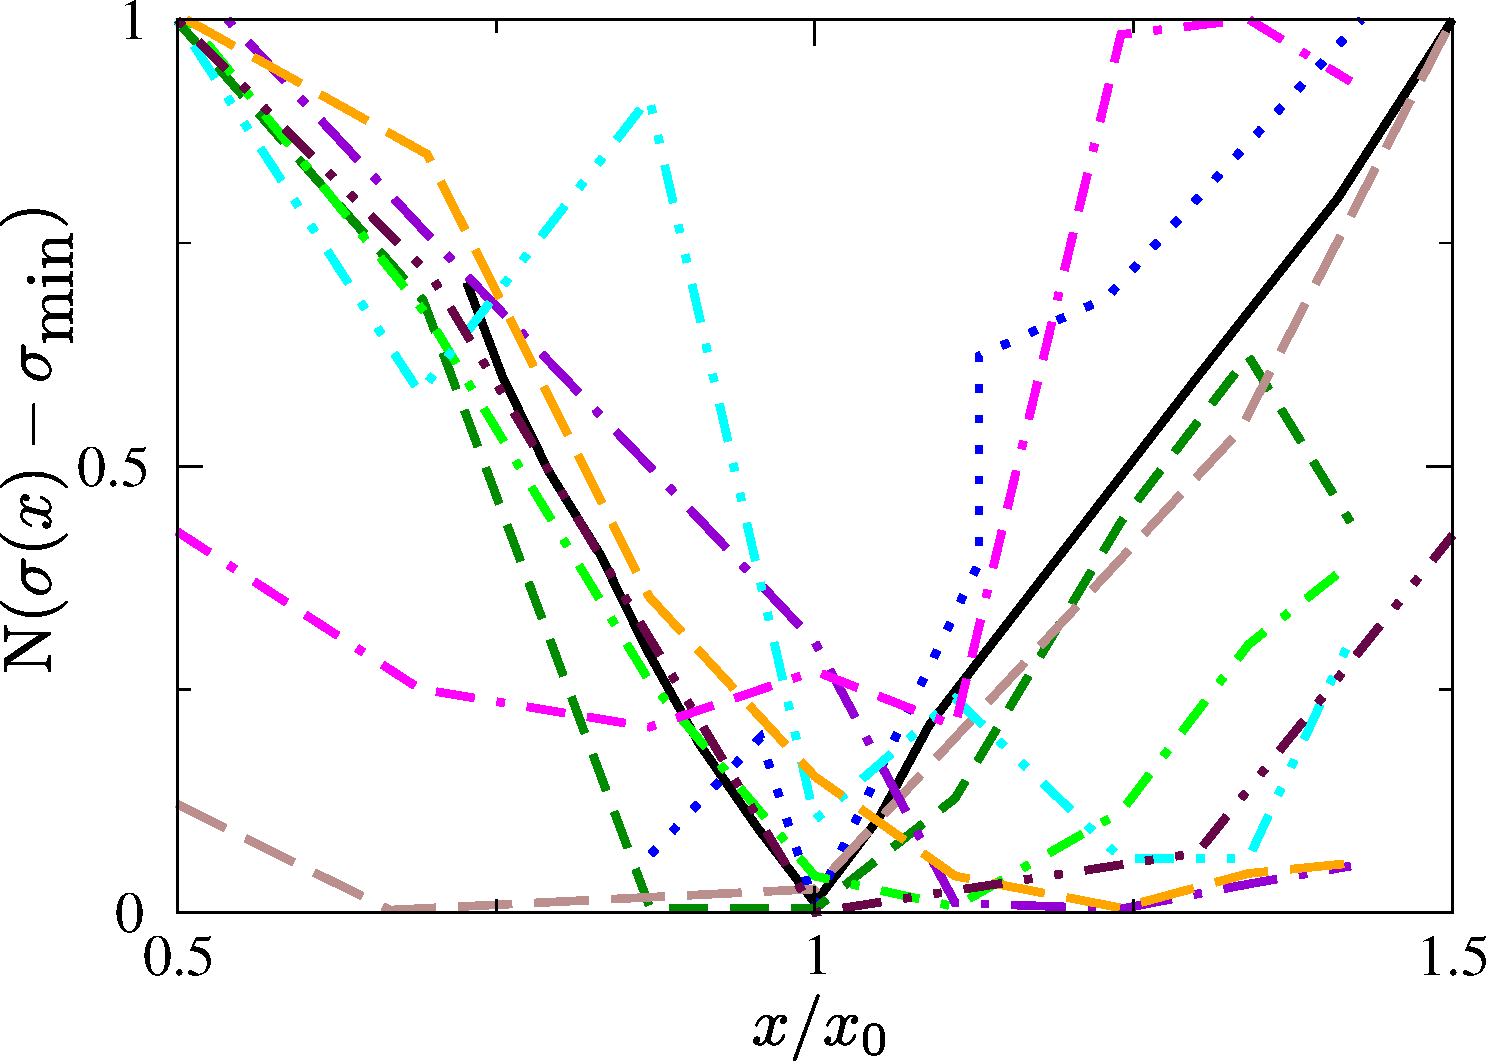
\includegraphics[width=0.8\textwidth]{introduccion/figs/funnel_norm_tot_try.pdf}
\caption{
Root mean square deviations $\sigma(x)$ (see Table 1) between theoretical predictions and experimental values of the different structural properties which ``completely'' characterise the open--shell nucleus $^{120}$Sn and involve the island of superfluid nuclei $^{118,119,120,121,122}$Sn, calculated as a function of $G$ (referred to $G_0 = 0.22 MeV$), $m_k$ ($(m_k)_0 = 0.7 m$), and $\beta_2$ ($(\beta_{2})_0 = 0.13$)  and in general to $x$ ($x_0$), measured with respect to the minimum value $\sigma_{\textrm{min}} = \sigma (x_{\textrm{min}})$, displayed in the interval $0.5 \leq x/x_0 \leq 1.5$ and normalized according to $0 \leq N(\sigma(x) - \sigma_{\textrm{min}}) \leq 1$.
The  curves represent: the deviation of the  pairing gap associated with the $h_{11/2}$ orbital 
($\Delta_{h_{11/2}} (G/G_0)$ (solid black curve);  
$\Delta_{h_{11/2}} (m_k/(m_k)_0)$ (dotted blue curve);  $\Delta_{h_{11/2}} (\beta_{2}/(\beta_{2})_0)$ (dashed green curve));
the deviation of the quasiparticle spectrum ($E_{qp}(G/G_0)$ (dashed brown curve);  $E_{qp}(\beta_{2}/(\beta_{2})_0)$ (dash-dotted green curve);
the deviation of the $h_{11/2}\otimes 2^+$ multiplet splitting  $E_{h_{11/2}\otimes 2^+}(\beta_{2}/(\beta_{2})_0)$ (dash-dotted purple curve); 
the deviation of the  centroid position of the $d_{5/2}$ strength function $S_{d_{5/2}}(\beta_{2}/(\beta_{2})_0)$ (dash-dotted cyan curve); 
the deviation of the width of the $d_{5/2}$ strength function  $S_{d_{5/2}} (\beta_{2}/(\beta_{2})_0)$ (dash-dotted pink curve);
the deviation  of the  quadrupole transition strength  $B(E2) (\beta_{2}/(\beta_{2})_0)$ (dashed orange curve). For details see \cite{Idini:15}.
The remarkable feature of the present figure is the fact that, in spite of the fluctuations of the results typical of finite  many--body systems, clearly defines a funnel in which all minima fall within a narrow window of $x/x_0$ values ($1 \pm 0.2$). This is a novel and unexpected result, which can be considered as an emergent property of a description of structure and reactions carried out in a basis of elementary modes of excitations, interacting through th PVC vertices according to the NFT rules.}\label{fig1.4.1x}
\end{center}
\end{figure}
\section{Non--orthogonality}\label{appintroC}
The ground state of $^{210}_{84}\text{Po}_{126}$ can be viewed as the proton pair addition mode of the doubly closed shell nucleus  $^{208}_{82}\text{Pb}_{126}$, mode displaying $J^\pi=0^+$ and $\beta=+2$ (transfer--) quantum numbers. Within this framework $^{209}_{83}\text{Bi}_{126}$ is expected to be a \emph{bona fide} proton single--particle system ($\beta=+1$), in which the $g_{7/2},d_{5/2},h_{11/2},d_{3/2}$ and $s_{1/2}$ valence orbitals are occupied, the odd proton occupying, in the ground state, a substate of the $h_{9/2}$ orbital.



This picture can be specifically probed through one--proton stripping and pick up reactions, e.g. with the help of $^{210}$Po$(t,\alpha)^{209}$Bi and $^{208}$Pb$(^3$He$,d)^{209}$Bi transfer processes\footnote{It is of notice that in the present case, as well as in Sect. \ref{appintroA}, and at variance with the rest of the monograph, use will be made, for the sake of being didactic, of spectroscopic factors, see end of Sect. \ref{C1S1}.}. The pick--up reaction cross section is, in the case of e.g. the states $1/2^+(s_{1/2})$ and $11/2^-(h_{11/2})$,  essentially consistent with a single peak displaying full $(2j+1)$ occupancy. On the other hand, two $3/2^+$ states with essentially equal strength and exhausting the associated $(2j+1(=4))$ strength are observed.   Furthermore,  the four peaks mentioned above are essentially not excited in the stripping process (see Table \ref{tabintroC1}). In an attempt to further clarify the structure of the two $3/2^+$, recur is made to the inelastic process $^{209}$Bi$(d,d')$. Both states are excited in the inelastic process, the associated  angular distributions  revealing the octupole character of such excitation (Tables \ref{tabintroC2} and \ref{tabintroC3}).

\begin{figure}
\centerline {
\includegraphics*[width=12cm]{introduccion/figs/figintroC1}
}
\caption{NFT diagram describing one of the most important processes coupling the $2p-1h$ states $\ket{\alpha}$ and $\ket{\beta}$ (see Eqs. (\ref{eqintroC1}) and (\ref{eqintroC2})), product of bare elementary modes of excitation consisting in the $^{208}$Pb, $0^+$ pair addition mode and the $d_{3/2}$ proton hole state, and of the lowest octupole vibration of $^{208}$Pb and of a proton moving in the $h_{9/2}$ orbital.}
\label{figintroC1}
\end{figure}
\begin{figure}
\centerline {
\includegraphics*[width=6cm]{introduccion/figs/figintroC2}}
\caption{Schematic representation of the $3/2^+$ states entering the NFT calculation of the process displayed in Fig. \ref{figintroC1}. The basis state $\ket \alpha$ carries the full $(t,\alpha)$ transfer strength ($tr$) $\sigma^{tr}$, while the basis state $\ket{\beta}$ the full octupole $(oct)$ strength $\sigma^{oct}$ (see Tables \ref{tabintroC1}--\ref{tabintroC3}). The overlap between these states is  $\cos \chi$. The physical states obtained through the (Feynman) diagramatic ``orthogonalization process'' are denoted $\ket{\text{I}}$ and $\ket{\text{II}}$ (see Eqs. (\ref{eqintroC3}) and (\ref{eqintroC4})).}
\label{figintroC2}
\end{figure}
In keeping with the fact that the same experiment reveals a multiplet (septuplet) of states with centroid around 2.6 MeV and with summed $L=3$ inelastic cross section consistent with that of the lowest collective  (2.615 MeV, $B(E3)/B_{sp}\approx 32$) octupole vibration of $^{208}$Pb, one can posit that the two $3/2^+$ states are a linear combination of the unperturbed (two particles)--(one hole) ($2p$--$1h$) states (see Fig. \ref{figintroC1}),
\begin{align}\label{eqintroC1}
\ket \alpha=\ket{d_{3/2}^{-1}\otimes gs (^{210}\text{Pb});3/2^+},
\end{align}
and 
\begin{align}\label{eqintroC2}
\ket \beta=\ket{h_{9/2}\otimes 3^- (^{208}\text{Pb});3/2^+}.
\end{align}
Because these states lie very close in energy they mix. According to NFT, the most important contribution to this mixing arises from the process given in Fig. \ref{figintroC1}. The resulting physical (mixed) states can be  written as,
\begin{align}\label{eqintroC3}
\ket {\text{I}}=-0.53 \ket \alpha + 0.76 \ket \beta,
\end{align}
and 
\begin{align}\label{eqintroC4}
\ket {\text{II}}=1.02 \ket \alpha + 0.80 \ket \beta,
\end{align}
as resulting from the calculation of the diagram displayed in Fig. \ref{figintroC1} to all orders of perturbation, with the help of Brillouin--Wigner perturbation theory (diagonalization of the corresponding effective Hamiltonian\footnote{See p. 316 \cite{Bortignon:77} and references therein.}. Let us now calculate the overlap $\mathcal O=\braket{\alpha|\beta}$ between the basis states $\ket\alpha$ and $\ket{\beta}$, that is $\mathcal O=\cos\chi$ (see Fig. \ref{figintroC2}).   
\begin{table}
\begin{tabular}{|c|c|c|c|}
\hline 
 & $E_x$(MeV) & $S(t,\alpha)(2j+1)$ & $S(^3\text{He},d)$ \\
 \hline 
$3/2^+$ & 2.49 & $1.8\pm0.3\,(4)$  & $<0.01$  \\ 
$3/2^+$ & 2.95 & $2.2\pm0.3\,(4)$  & $<0.01$ \\ 
 $1/2^+$& 2.43 &  $1.8\,(2)$& $<0.02$ \\ 
 $11/2^-$& 3.69 & $10\,(12)$ &  $<0.05$\\ 
 \hline
\end{tabular}\caption{Single--particle strength associated with the single--particle transfer reactions  $^{210}$Po$(t,\alpha)^{209}$Bi and $^{208}$Pb$(^3\text{He},d)^{209}$Bi (see \cite{Bortignon:77}).}\label{tabintroC1}
\end{table}
\begin{table}
\begin{tabular}{|c|c|c|}
\hline 
 & & $\frac{\sigma\left(^{209}\text{Bi}(9/2^-;gs)\rightarrow^{209}\text{Bi}(3/2^+;E)\right)}{\sigma\left(^{208}\text{Pb}(gs)\rightarrow (3^-;2.615\, \text{MeV})\right)}$  \\
 \hline 
$3/2$ & 2.49 & $0.041\pm0.003$   \\ 
$3/2$ & 2.95 & $0.011\pm0.002$  \\ 
 \hline
\end{tabular}\caption{The total inelastic cross section $\sigma^{oct}$ associated with the lowest octupole vibrational state of $^{208}$Pb can be written in terms of that associated with a single magnetic substate $\sigma'$ as $\sigma_{3^-}^{oct}=7\sigma'$. That associated with the multiplet $(h_{9/2}\otimes 3^-)_{J^+} (J=3/2-15/2)$ as $\sigma_{3^-}^{oct}=70\sigma'$, in keeping with the fact that the $h_{9/2}$ state has 10 magnetic substates. Thus, the strength associated with the 3/2 channel is 4/70=0.057 to be compared with the observed summed (percentage) strength $0.053\pm0.005 $ $(=(0.042\pm0.003)+(0.011\pm0.002))$ associated with the 2.45 MeV and the 2.95 MeV $3/2^+$ states; see \cite{Bortignon:77}.}\label{tabintroC2}
\end{table}
\begin{table}
\begin{tabular}{|c|c|c|c|c|c|c|c|c|}
\hline
& \multicolumn{2}{|c}{$E_n$(MeV)} & \multicolumn{2}{|c}{$\frac{\sigma(h_{9/2}\rightarrow 3/2^+)}{\sigma(0^+\rightarrow 3^-)}$(\%)} & \multicolumn{2}{|c}{$S(t,\alpha)$}  & \multicolumn{2}{|c|}{$S(^3\text{He},d)$}   \\
\hline
&Theory  & Exp  & Theory  & Exp & Theory & Exp & Theory  & Exp  \\
\hline
3/2& 2.480 & 2.494  & 3.76  & $4.2\pm0.3$  & 1.83  & $1.8\pm0.3$ &0.02  & $<0.01$  \\
3/2& 3.125 & 2.95  & 1.56 & $1.1\pm0.2$  & 2.25  & $2.2\pm0.3$ & $10^{-5}$  & $<0.01$  \\
\hline
\end{tabular}\caption{Summary of NFT predictions concerning the structure of the two lowest $3/2^+$ state of $^{209}$Bi, in comparison with the experimental data (see Table 4.7 of \cite{Bortignon:77}).}\label{tabintroC3}
\end{table}
Following this figure  one can write,
\begin{align}
\sqrt{\sigma_I^{tr}}=\cos\phi;\quad \sqrt{\sigma_{II}^{tr}}=\cos\left(\frac{\pi}{2}-\phi\right)=\sin \phi,
\end{align}
where
\begin{align}
{\sigma^{tr}}={\sigma_I^{tr}}+{\sigma_{II}^{tr}}=1,
\end{align}
in keeping with the fact that the absolute cross sections of the states $\ket {\text{I}}$ and $\ket {\text{II}}$ are normalized in terms of the total cross section (see caption to Fig. \ref{figintroC2}).


In the same way
\begin{align}
\sqrt{\sigma^{oct}_I}=\cos(\chi-\phi)=\cos\chi\cos\phi+\sin\chi\sin\phi,
\end{align}
and
\begin{align}
\sqrt{\sigma^{oct}_{II}}=\cos\left(\pi-\left(\frac{\pi}{2}-\phi+\chi\right)\right)=-\cos\left(\frac{\pi}{2}+(\phi-\chi)\right)=\sin\phi\cos\chi+\sin\chi\cos\phi.
\end{align}
Thus
\begin{align}
\sqrt{\sigma^{oct}_{I}}=\cos\chi\sqrt{\sigma^{tr}_{I}}+\sin\chi\sqrt{\sigma^{tr}_{II}},
\end{align}
and
\begin{align}
\sqrt{\sigma^{oct}_{II}}=-\cos\chi\sqrt{\sigma^{tr}_{II}}+\sin\chi\sqrt{\sigma^{tr}_{I}}.
\end{align}
Multiplying the above relations by $\sqrt{\sigma^{tr}_{I}}$ and $\sqrt{\sigma^{tr}_{II}}$ respectively one obtains,
\begin{align}
\sqrt{\sigma^{tr}_{I}\sigma^{oct}_{I}}=\cos\chi\sigma^{tr}_I+\sin\chi\sqrt{\sigma^{tr}_{I}\sigma^{tr}_{II}},
\end{align}
and
\begin{align}
\sqrt{\sigma^{tr}_{II}\sigma^{oct}_{II}}=-\cos\chi\sigma^{tr}_{II}+\sin\chi\sqrt{\sigma^{tr}_{I}\sigma^{tr}_{II}},
\end{align}
which, upon substraction  leads to the  expression of the overlap
\begin{align}
\cos\chi=\frac{\sqrt{\sigma^{tr}_{I}\sigma^{oct}_{I}}-\sqrt{\sigma^{tr}_{II}\sigma^{oct}_{II}}}{\sigma_I^t+\sigma_{II}^t}.
\end{align}
Making use of the values of Tables \ref{tabintroC1}--\ref{tabintroC3} (see also Fig. \ref{figC1A7} (e) last column labeled \textit{experiment})\footnote{See Table 4.7 of \cite{Bortignon:77}.} one obtains
\begin{align}
\cos\chi=\frac{\sqrt{1.8\times4.2}-\sqrt{2.2\times1.1}}{4}=0.298
\end{align}
  Simple estimates of the NFT prediction can be made making use of the relations\footnote{see Table 4.6 \cite{Bortignon:77}.}.
\begin{align}
\nonumber &\braket{\text{I}|\text{I}}= (-0.53)^2+(0.76)^2-2\times0.53\times0.75\, \mathscr O=1,\\
\nonumber &\braket{\text{II}|\text{II}}= (1.02)^2+(0.80)^2+2\times1.02\times0.80\, \mathscr O=1,
\end{align}
and $\braket{\text{I}|\text{II}}=-0.53\times1.02+0.76\times0.80+(-0.53\times0.80+0.76\times1.02)\,\mathscr O=0$ leading to $\mathscr O=-0.18, -0.42$ and -0.19 respectively and, thus, to the average value of \mbox{$-0.26$}.
 Of course, one can hardly expect to obtain the sign to agree with that of the NFT expression, as it is associated with a free choice of the axis of references (Fig. \ref{figintroC2}) (note also the fact that the quantities $\sigma$ appearing above are well defined, while $\sqrt{\sigma}$ is undetermined by an overall sign).
\section{Coupling between intrinsic and relative motion}\label{appintroB}
In what follows, we consider the reaction
\begin{align}
a+A\rightarrow b+B,
\end{align}
within the framework of the semiclassical approximation\footnote{\cite{Broglia:04a} and references therein.}.
In the center--of--mass system, the local Hamiltonian may be written
\begin{align}\label{eqintroB2}
H=T_{aA}+H_a+H_A+V_{aA}=T_{bB}+H_b+H_B+V_{bA},
\end{align}
in keeping with energy conservation. Within this context other, mixed, representations are possible.

One then solves the time--dependent Schr\"odinger equation 
\begin{align}
i\hbar\frac{\partial \Psi}{\partial t}=H\Psi,
\end{align}
with the initial conditions that the nuclei $a$ and $A$ are in their ground states, and where the relative motion is described by a narrow wavepacket of rather well defined impact parameter and velocity.


We expand $\Psi$ on (stationary) channel wavefunctions 
\begin{align}
\Psi=\sum_{\beta}c_\beta\left(\left(\mathbf r_\beta-R_\beta\right)\right)\Psi_\beta e^{-iE_\beta t/\hbar},
\end{align}
where
\begin{align}
\Psi_\beta (t)=\Psi_m^b(\xi_b)\Psi_n^B(\xi_B)\exp(i\delta_\beta).
\end{align}
The index $\beta$ labels both the partition of nuclei $(b,B)$ as well as the quantal states of the two nucleons ($m,n$).


The phase $\delta_\beta$ is defined as
\begin{align}
\delta_\beta=\frac{1}{\hbar}\left\{m_\beta \mathbf v_\beta(t)\cdot \left(\mathbf r_\beta-\mathbf R_\beta(t)\right)-\int_0^t\left(U_\beta\left(R_\beta(t')\right)-\frac{1}{2}m_\beta\mathbf v_\beta(t')^2\right)\right\}.
\end{align}
 Where an extra phase has been added to eliminate, as far as possible, the diagonal matrix elements in the coupled equations.
The phase factor $\exp(i\delta_\beta)$ acting on the channel wavefunction is essentially a Galilean transformation (see jagged ``phonon'' in the NFT reaction diagrams displayed in Figs. \ref{fig6.1.1} (one--particle transfer) and \ref{figC7C1} and \ref{figC7C2} (two--particle transfer); see also Figs. \ref{figintro2} and \ref{figintro3}).



The function $c_\beta$ can be expressed as
\begin{align}
c_\beta=a_\beta(t)\chi_\beta(\mathbf r_\beta-\mathbf R_\beta(t),t)
\end{align}
product of an amplitude $a_\beta$ of asymptotic values ($t=\pm\infty$, 0 or 1), and a normalized shape (wavepacket) function, $R_\beta(t)$ being the relative motion elastic trajectory.


Properly combining the above quantities and making use of the time--dependent Schr\"odinger equation one obtains 
\begin{align}
i\hbar\sum_{\beta}\dot a_\beta(t)\langle\Psi_\xi|\Psi_\beta\rangle_{\mathbf R_{\xi\gamma}}e^{iE_\beta t/\hbar}=\sum_{\gamma}\langle\Psi_\xi|V_\gamma-U_\gamma(r_\gamma)|\Psi_\gamma\rangle_{\mathbf R_{\xi\gamma}}a_\gamma(t)e^{iE_\beta t/\hbar},
\end{align}
where
\begin{align}
f(\mathbf R)=\langle\Psi_\xi|V_\gamma-U_\gamma(r_\gamma)|\Psi_\gamma\rangle_{\mathbf R}
\end{align}
are the formfactors, and
\begin{align}
g(\mathbf R)=\langle\Psi_\xi|\Psi_\beta\rangle_{\mathbf R}
\end{align}
the overlaps between the intrinsic channel wavefunctions.



The coupled equations can be written in a more compact form by introducing the adjoint channel wavefunction 
\begin{align}
\omega_\xi=\sum_{\gamma}g_{\xi\gamma}^{-1}\Psi{\gamma},
\end{align}
where $g^{-1}$ is the reciprocal of the overlap matrix
\begin{align}
g_{\xi\gamma}=\langle\Psi_\xi|\Psi_\gamma\rangle.
\end{align}
Thus
\begin{align}
(\omega_\xi,\Psi_\beta)=\delta(\xi,\beta),
\end{align}
and
\begin{align}
i\hbar\dot a_\beta(t)=\sum_{\gamma}\langle\omega_\beta|V_\gamma-U_\gamma|\Psi_\gamma\rangle_{\mathbf R_{\beta\gamma}}e^{(E_\beta-E_\gamma)t/\hbar}a_\gamma(t).
\end{align}
Consequently, the proper tunneling Hamiltonian is obtained by a basis orthogonalization process. These coupled equations, being first order in time, can be solved knowing the initial conditions at time $t=-\infty$,
\begin{align}
a_\gamma(-\infty)=\delta(\gamma,\alpha),
\end{align}
where $\alpha$ labels the entrance channel, that is, the nuclei $a$ and $A$ in their ground state. The cross section for the reaction $\alpha\rightarrow\beta$ is
\begin{align}
\left(\frac{d\sigma}{d\Omega}\right)_{\alpha\rightarrow\beta}\sim\left|a_\beta(t=+\infty)\right|^2,
\end{align}
Let us now  solve the coupled equations in first order perturbation theory. For this purpose we insert $\delta(\gamma,\alpha)$ at the place of $a_\gamma(t)$ obtaining 
\begin{align}\label{eqintroB17}
\nonumber a_\beta(t)&=\frac{1}{i\hbar}\int_{-\infty}^{t}\langle\omega_\beta|V_\alpha-U_\alpha|\Psi_\alpha\rangle_{\mathbf R_{\beta\alpha}(t)}\exp^{i(E_\beta-E_\alpha)t'/\hbar}dt'\\
&=\frac{1}{i\hbar}\int_{-\infty}^{t}dt'\langle\Psi_\beta|V_\alpha-U_\alpha|\Psi_\alpha\rangle_{\mathbf R_{\beta\alpha}(t)}\exp^{i(E_\beta-E_\alpha)t'/\hbar}
\end{align}
where the expansion,
\begin{align}\label{eqintroB18}
\omega_\beta=\Psi_\beta-\braket{\Psi_\alpha|\Psi_\beta}_{\mathbf R_{\beta\alpha}(t)}
\end{align}
has been used, and the ansatz made, that the
 global optical potentials ($U$: real part), and standard nucleon--nucleon interactions $V$  fulfill the relation
\begin{align}
\braket{\Psi_\alpha|V_\alpha-U_\alpha|\Psi_\alpha}=0.
\end{align}
It is of notice that the overlap appearing in Eq. (\ref{eqintroB18}) can, in the case of a two--particle transfer reaction 
\begin{align}
\alpha\equiv a (=b+2)+A\rightarrow b+B(=A+2)\equiv\beta,
\end{align}
contribute with an amplitude $\braket{\Psi_\beta|\idop|\Psi_\gamma}\braket{\Psi_\gamma|V_\alpha-U_\alpha|\Psi_\alpha}$, where $\idop$ is the unit operator, while $\gamma\equiv f(=b+1)+F(=A+1)$, denotes the mass partition of the intermediate channel. The above expression strongly suggests that a consistent description of two--transfer reactions in a non--orthogonal basis involves, at least, three strongly interweaved  reaction channels (as testified by the fact that they can be shifted around by changing representation, that is post--post, prior--prior, and prior--post, see e.g. Eq. (\ref{eqintroB2}) as well as Fig. \ref{figC7C2}), namely $\alpha,\gamma$ and $\beta$ and consequently has to be calculated, at least, to second order of perturbation theory, that is, including simultaneous and successive transfer and non--orthogonality corrections.

Let us now return to the sum--rule subject considering,  for simplicity, the simultaneous transfer amplitude (\ref{eqintroB17}) (see also Sect. \ref{C7AppC} Eq. \ref{eq7.C.4}). That is,
\begin{align}\label{eqintroB19}
\nonumber a^{(1)}(t=+\infty)&=\frac{1}{i\hbar}\int^{\infty}_{-\infty}dt\exp^{\left[\frac{i}{\hbar}(E^{bB}-E^{aA})t+\gamma_{\beta\alpha}(t)\right]}\\
&\times\braket{\phi^{B(A)}(\mathbf r_{1A},\mathbf r_{2A})|U(r_{1b})|e^{\sigma_{\beta,\alpha}}\phi^{a(b)}(\mathbf r_{1b},\mathbf r_{2b})}_{\mathbf R_{\alpha\beta}(t)},
\end{align}
where
\begin{align}
\sigma_{\beta,\alpha}=\frac{1}{\hbar}\frac{m_n}{m_A}(m_{aA}\mathbf v_{aA}(t)+m_{bB}\mathbf v_{bB}(t))\cdot(\mathbf r_\alpha-\mathbf r_\beta),
\end{align}
takes care of recoil effects, the phase factor $e^{\sigma_{\beta,\alpha}}$ being a generalized Galilean transformation associated with the mismatch between entrance and exit channels,  while the phase
\begin{align}\label{eqintroB21}
\nonumber\gamma_{\beta\alpha}(t)&=\int^t_0 dt'\left\{U_\beta(\mathbf R_{\beta}(t'))-\frac{1}{2}m_\beta v_\beta^2(t')-U_\alpha(\mathbf R_\alpha(t'))+\frac{1}{2}m_\alpha v_\alpha^2(t')\right\}\\
&+\frac{1}{2\hbar}\left(m_\alpha \mathbf v_\alpha(t)+m_\beta \mathbf v_\beta(t) \right)\cdot(\mathbf R_\beta(t)-\mathbf R_\alpha(t)),
\end{align}
is related to the effective $Q$--value of the reaction.


The rate of change of the formfactor $\braket{\phi^{B(A)},U(r_{1b})e^{i\sigma{\beta\alpha}}\phi^{a(b)}}$ with time is slow, being completely overshadowed by the rapidly varying phase factor\\ $\exp\left[\frac{i}{\hbar}(E^{bB}-E^{aA})t+\gamma_{\beta\alpha}(t)\right]$. Similar relations concerning recoil and $Q$--value effects can be obtained from the amplitudes associated to successive and to non--orthogonality terms i.e. $a^{(2)}(\infty)$ and $a^{(NO)}$ (see Ch. \ref{C7}, Sect. \ref{C7AppC}).


Summing up, to compare two--nucleon transfer cross sections on equal structural footing, one has to eliminate the kinematical oscillating phase which can completely distort the ``intrinsic'' (reduced matrix element) value of the two--nucleon cross section. And for that, one has to work on each of the three amplitudes to extract at best the phases which couple relative and intrinsic motion.



Let us make a parallel with the sum rule associated with electromagnetic decay (Coulomb excitation, $\gamma$--decay). The absolute transition probability for absorption (emission) of a photon from nuclear dipole states is measured in sec$^{-1}$ by (\cite{Bohr:69})
\begin{align}
T(E1)=\left(1.59\times 10^{15}\right)\times (E)^3\times B(E1),
\end{align}
where $E$ is the energy of the transition and $B(E1)$ the reduced transition probability. It is this quantity that enters the TRK--sum rule,
\begin{align}
S(E1)=\bra{0}[[H,\mathcal M(E1)]],\mathcal M(E1)]\ket{0}/2,
\end{align}
 and not $T(E1)$. Now, in this particular case the $Q$--value dependence of the observed absolute transition probabilities can be eliminated analitically ($E^3$ dependence), as well as the overall factor  ($1.59\times 10^{15}$), in keeping with the fact that the mass partition ($a+A\rightarrow a+A^*$) as well as the overall factor does not change between entrance and exit channels or, equivalently, the coordinate of relative motion $\mathbf R_{\alpha\alpha'}(t)$ is always that describing the relative center of mass position of target and projectile. This fact allows for a complete separation between structure and reaction (kinematics), explicit in the general expression of $T(E\lambda)$, that is,
 \begin{align}
 T(E\lambda;I_1\rightarrow I_2)=\left(\frac{8\pi(\lambda+1)}{\lambda[(2\lambda+1)!!]^2}\frac{1}{\hbar}q^{2\lambda+1}\right)\left(B(E\lambda;I_1\rightarrow I_2)\right),
 \end{align}
where $\mathbf q$ is the momentum of the photon, and 
 \begin{align}
B(E\lambda;I_1\rightarrow I_2)=\frac{\braket{I_2||\mathcal M(E\lambda)||I_1}}{\sqrt{2I_1+1}},
 \end{align}
 the reduced transition probability. Thus, the first factor in the expression of $T(E\lambda)$ contains all the kinematics (reaction) of the process, the second  one the nuclear structure part of it. In the above relation, the multipole tensor is defined as,
 \begin{align}
\mathcal M(E\lambda,\mu)=\int \rho(\mathbf r)r^\lambda Y_{\lambda\mu}(\hat r)d \mathbf r.
 \end{align}
It is of notice that the non--diagonal elements (transition moments) are involved in electric $\rho_e$ and nuclear ($\rho$) multipole processes ($\gamma$--decay, Coulomb excitation, inelastic scattering, etc.).



Returning to the expression of the first order (simultaneous) two--nucleon transfer amplitude $a^{(1)}(t=+\infty)$ one can only devise empirical protocols to try to extract the $\gamma$-- and $\sigma$--phase dependence (see Eqs. (\ref{eqintroB19})--(\ref{eqintroB21})) from it and set all absolute two--nucleon transfer cross sections $d\sigma/d\Omega\sim |a|^2$ on equal footing regarding kinematics, so as to allow to compare the intrinsic, reduced transition probabilities (structure). In other words, extract the structure information contained in, e.g.,
 \begin{align}
\phi^{B(A)}(\mathbf r_{1A},\mathbf r_{2A})=\braket{\mathbf r_{1A},\mathbf r_{2A}|\Gamma^\dagger_1(\beta=+2)|\tilde 0},
 \end{align}
where
 \begin{align}
\Gamma_n^\dagger(\beta=+2)=\sum_k X_k^n\left[a^\dagger_ka^\dagger_k\right]_0-\sum_i Y^n_i \left[a_i a_i\right]_0,
 \end{align}
is the pair creation addition mode acting on of a closed shell system $\ket{\tilde 0}$, as well as in
 \begin{align}
\phi^{B(A)}(\mathbf r_{1A},\mathbf r_{2A})=\bra{\mathbf r_{1A},\mathbf r_{2A}}\left[a^\dagger_ka^\dagger_k\right]_0\ket{0},
 \end{align}
that is, in the pure two--particle configuration $\ket{j^2_k(0)}$ describing two nucleons moving in time reversal states of the close shell system $\ket 0$. If one was able to disentangle the $\gamma$ and $\sigma$ dependence of $a^{(1)}$ (as well as that of $a^{(2)}$ and $a^{(NO)}$, see above) from its formfactor dependence, the comparison between the quantities $\sum_n|c^{(n)}|^2$, $\sum_k|X^{(n)}_k|^2$ and $\sum_i|Y^{(n)}_i|^2$ could  eventually be phrased in terms of exact sum rules. This not being  the case, one has to  deal with approximate TNTR sum rules. With this proviso in mind, TNTR sum rules are nonetheless quite useful.
\section{Nuclear Field Theory for pedestrians}\label{appintroA}
%In a classical world, empty space is the absence of physics, and the existence of something, e.g. of light or of  an electron is only a clue to eventually learn what the ``object'' can be: wave or particle. Think only on all the work concerning the vibrations of an hypothetical ``aether'', or concerning the ``divergent'' mass (energy) of the electron. Within this last context, the same is somewhat true in quantum mechanics, with a small difference. We do not need to think whether light is a particle or a wave. But yes, whether it is a composite particle or less, in both the sense of finite lifetime or coupling to other particles.  Namely, what are the values of the parameters characterizing the bare particles (e.g. $m$) so that the dressed ones reproduce the experimental findings.


Nuclear Field Theory (NFT) was tailored after Feynman's graphical version of quantum electrodynamics (QED). It is then natural that in discussing NFT analogies with QED will be recurrent. Pairing is important in atomic nuclei, and Cooper pairs play a central role both in open and in closed shell nuclei. In the first case through condensation and superfluidity, closely connected with the observation of pairing rotational bands. In the second case, through collective pairing vibrations which change particle number in two\footnote{For details concerning pairing rotations and vibrations we refer to \cite{Bes:77} and \cite{Brink:05} Chs. 4 and 5 respectively, and refs. therein.}. It is then also natural that references to BCS and Cooper condensation and tunneling are widely used in this monograph\footnote{Within this context see \cite{Broglia:13}}. Arguably, as a consequence of special relativity which put an end to the concept of ether, the field--free and matter--free vacuum was rightly considered as \textit{bona fide} empty space. The advent of quantum mechanics changed this situation, the vacuum becoming populated. In quantum mechanics an oscillator, for example, cannot be at rest. The oscillatory nature of the radiation field requires zero point fluctuations (ZPF) of the electromagnetic fields in the vacuum state of lower energy. The occupation of the negative kinetic energy electron states and the subsequent calculation of the cross section for pair creation by photons in the Coulomb field of atomic nuclei, (the nuclear particle--hole excitations), contribute another step in the understanding of the QED vacuum.


When the fields are expressed in terms of creation and annihilation operators, the fermion and boson fields in its simple form consists on the product of two fermion creation or destruction operator $a^\dagger$ or $a$ and one boson operator $\Gamma^\dagger$ or $\Gamma$: e.g. $a^\dagger_{\nu'}a_\nu\Gamma_\alpha^\dagger$, (see Fig. \ref{figintroA1}). That is,  bilinear in the fermion fields and linear in the boson fields.

\begin{figure}
\centerline {
\includegraphics*[width=8cm]{introduccion/figs/figintroA1}
}
\caption{Oyster diagrams describing the correlation of the nuclear ground state associated with the ZPF of a collective particle--hole excitation is built, and Pauli principle correction processes in which fermions are exchanged.}
\label{figintroA1}
\end{figure}
\begin{figure}
\centerline {
\includegraphics*[width=10cm]{introduccion/figs/figintroA2}
}
\caption{Some of the possible outcomes resulting from acting with a single--particle field, e.g. that associated with inelastic processes (represented by a horizontal dashed line starting with a $\times$), on the Pauli corrected ZPF oyster diagrams associated with collective $(p-h)$ excitations of the nuclear vacuum (see also Fig. \ref{figintroA1}). It is of notice the care with which the contribution of the collective states have to be selected, only ones which can be accurately calculated. Within this context one returns to the question of empirical renormalization mentioned in the text (see Sect. \ref{C1S4}, cf. also \cite{Idini:15}, \cite{Broglia:16}).}
\label{figintroA2}
\end{figure}
\clearpage
\begin{figure}[h!]
\centerline {
\includegraphics*[width=10cm]{introduccion/figs/figintroA3}
}
\caption{ZPF associated with the pair addition mode taking into account the interweaving of nucleons with density modes. The processes boxed in (g), (k) and (o), are associated with the induced pairing interaction (medium polarization effects; (p), (q), (r)) resulting from the exchange of density modes between nucleons moving in time reversal states. The two--nucleon stripping and pickup external field is labeled by a dashed horizontal line which starts with a $\times$.}
\label{figintroA3}
\end{figure}
\clearpage

A detailed graphical NFT treatment of the vacuum has an important consequence concerning the probing of nuclear structure with reactions. By intervening it with an external field one will excite the modes whose properties can be eventually compared with experiment without further ado. 

In other words, if one is in doubt of which are the properly dressed elementary, physical modes of excitation, do not study them, or calculate them and then compare the results with the experimental data. This comes after. One should first find out how to specifically excite the  mode in question, by acting with an external field on the ZPF of the vacuum. That is, by carrying out a \textit{gedanken}, NFT--like \textit{experiment} as in Fig. \ref{figintroA2} for $p-h$--vibrations and in Fig. \ref{figintroA3} regarding pairing vibrations. Because the corresponding processes deal  with physical states, they translate with ease into a laboratory setup. In keeping with the fact that the vacuum contains all the information (right physical degrees of freedom) of the quantal system under study, forcing virtual processes associated  with vacuum ZPF to become real, one is guaranteed to get, in each instance, the real, dressed, physical particle. Of course, once the \emph{gedanken eksperiment} has provided this information, one should use such properly renormalized modes, in all the rest of the calculations, at the risk of neglecting relevant physics. 


Let us now provide a short introduction of NFT for pedestrians and see how the above considerations become concretely implemented\footnote{For details we refer to \cite{Bortignon:77} and refs. therein.}
\subsection[The concept of elementary modes of excitation]{The concept of elementary modes of excitation\protect\footnote{\cite{Bes:77}}}\label{C1S7.1}
The Hamiltonian of a many--body system of noninteracting particles, bosons or fermions, can be written as
\begin{align}\label{eqC1A1}
H=\sum_iH_i,
\end{align}
where the summation is over all the particles of the system and where each $H_i$ depends only on the variables of the $i$--th particle. The single--particle Schr\"odinger equation is
\begin{align}\label{eqC1A2}
H_i\psi_k(\mathbf r_i)=\epsilon_k \psi_k(\mathbf r_i),
\end{align}
where $\epsilon_k$ is the single--particle energy eigenvalue and 
\begin{align}\label{eqC1A3}
\psi_k(\mathbf r_i)\equiv\bra{\mathbf r_i}a_k^\dagger\ket{0}
\end{align}
is the corresponding wave function. The operator $a_k^\dagger$ creates a particle in the state $k$ when acting in the vacuum state $\ket{0}$. The energy levels of the system are given by the equation
\begin{align}\label{eqC1A4}
E_n=\sum_k n_k\epsilon_k,
\end{align}
the corresponding eigenstates being
\begin{align}\label{eqC1A5}
\ket{n}=\prod_k\frac{(a_k^\dagger)^{n_k}}{\sqrt{n_k!}}\ket{0},
\end{align}
where $n_k=0$ or 1 in the case of fermions and $n_k=0,1,2,\dots$ in the case of bosons.

Now we consider a system of interacting particles. The Hamiltonian will in this case be
\begin{align}\label{eqC1A6}
H=\sum_i H_i+\frac{1}{2}\sum_{i,j}H_{ij},
\end{align}
where $i,j$ label the co--ordinates of the $i$--th and $j$--th particle.

In some cases it is possible to recast the two--body Hamiltonian in the form
\begin{align}\label{eqC1A7}
H=\sum_r H'_r,
\end{align}
with the associated Schr\"odinger equation
\begin{align}\label{eqC1A8}
H'_r\psi_r(\zeta)=\epsilon_r \psi_r(\zeta),
\end{align}
$\zeta$ representing a general variable (e.g. the single--particle co--ordinate, the gap parameter, the shape of the nucleus, etc.). The wave function $\psi_r(\zeta)$ is the $\zeta$--co--ordinate representation of the eigenstate $\alpha_\tau^\dagger\ket{\tilde 0}$. The operator $\alpha_\tau^\dagger$ creates an excitation with the quantum number $\tau$ when acting in the state $\ket{\tilde 0}$, the vacuum of all the excitations $\tau$.



The energy of the levels of the system, or at any rate of the most important
ones to determine the physical response of it to external probes, can be written
in the form
\begin{align}\label{eqC1A9}
E_m=\sum_{\tau}n_\tau \epsilon_\tau
\end{align}
The corresponding eigenstate can be written in the same way as before, \textit{i.e.}
\begin{align}\label{eqC1A10}
\ket{n}=\prod_\tau\frac{(a_\tau^\dagger)^{n_\tau}}{\sqrt{n_\tau!}}\ket{\tilde 0}.
\end{align}
Additivity features similar to (\ref{eqC1A9}) hold for other physical quantities, \textit{i.e.}
\begin{align}\label{eqC1A11}
\braket{n|\mathcal O|m}=\sum_{\tau}A_\tau\sqrt{n_\tau} \delta(n_\tau,m_\tau+1),
\end{align}
where
\begin{align}\label{eqC1A12} O=\sum_{\tau}A_\tau \alpha_\tau^\dagger
\end{align}
is the operator which specifically excites the eigenstates described by $\psi_\tau(\xi)$.
Because the excitation energies $E_m$ and observables $\left|\braket{m'|\mathcal O|m}\right|^2$ (e.g. two--particle transfer cross--section, electromagnetic-transition probabilities, etc.) are
linear combinations of $\epsilon_\tau$ and $A_\tau$, respectively, the eigenstates with energy $\epsilon_\tau$
and associated observable $A_\tau$ are called the \textit{elementary excitations of the system}.


There lie thus two ideas behind the concept of elementary excitations \footnote{This concept was first introduced ,by Landau \citep{Landau:41} to describe the spectrum
of HeII. lt was subsequently utilized in nuclear physics by Bohr and Mottelson \cite{Bohr:69,Bohr:75}
to obtain a unified description of the nuclear spectrum.}.
First, there is the idea that the total binding energy, although an important quantity by itself, does not have much to do
with the behaviour of the physical system. Thus, the state $\ket{\tilde 0}$ is assumed to
exist but to act only as a background whose detailed intrinsic structure one does
not need to know to describe the behaviour of the system. What is important
is the behaviour of the lower excited states relative to the ground state.
The second idea is that the low--lying states often are of a particular simple
character, and are amenable to a simple and rigorous mathematical treatment.
With the help of experimental probes which couple weakly to the nucleus,
i.e. in such a way that the system can be expressed in terms of the properties
of the excitation in the absence of probes, it has been possible to identify the
following' elementary excitations in systems around closed shells\footnote{The restriction to closed shell nuclei is made to simplify the discussion. The concept
of elementary modes of excitation applies equally well to open-shell nuclei.}:
\begin{enumerate}[a)]
\item single particle and holes,
\item shape vibrations,
\item spin and isospin vibrations and charge exchange modes,
\item pairing vibrations.
\end{enumerate}
Away from closed shells one has to add to the above modes:
\begin{enumerate}[a)]
\setcounter{enumi}{4}
\item rotations in 3D--space (e.g. quadrupole rotations)
\item rotations in gauge space (pairing rotations).
\end{enumerate}
Different probes have been utilized in the process of the identification of the different modes. In particular two-neutron transfer reactions induced by tritons
and protons have played a central role in unraveling the basic features of the pairing modes. 
\subsection{NFT rules and applications}\label{Sect1.7.2}
A field theory can be formulated in which the nuclear elementary modes of
excitation play the role of the free fields and in which their mutual interweaving takes place through the particle--vibration coupling vertices\footnote{\cite{Bohr:75,Bes:74,Broglia:76}.}.
This theory provides a graphical perturbative approach to obtain the exact
solution of the many-body nuclear-structure problem in the product basis $\psi_\tau(\zeta)\psi_\eta(\Delta)\dots\psi_\gamma(\Gamma)$


Note that the nuclear bosonic fields are built out by utilizing those degrees
of freedom (particles and holes) which already exhaust all the nuclear degrees
of freedom. It is thus an essential feature of the product basis to be over-
complete and to violate the Pauli principle. On the other hand, this basis is
directly related to observables of the system. The different experiments project out only one or two of its components.


In what follows we state and apply the nuclear-field-theory rules, to calculate the interactions between the nuclear free fields and the reaction processes
between the resulting physical states. This is done for a system with one particle outside closed shells and which displays collective vibrations, in the framework of a two--level model.
\subsubsection{Schematic model}
The model considered consists of two single--particle levels, each with degeneracy\footnote{It is of notice the difference of a factor of 2 in the degeneracy of each level as compared to Sect. 2 of \cite{Bortignon:77} in which case it is $2\Omega$. This is in keeping with the fact that, as a rule, $\Omega=(2j+1)/2$.} $\Omega$ and with a schematic monopole particle--hole interaction coupling the particles in the two levels.

The total Hamiltonian is equal to
\begin{align}\label{eqC1A13} 
H=H_{sp}+H_{TB}
\end{align}
where
\begin{align}\label{eqC1A14} 
H_{sp}=\frac{\epsilon}{2}N_0,\quad\quad N_0=\sum_{\sigma=\pm 1,m}\sigma a^{\dagger}_{m,\sigma}a_{m,\sigma},
\end{align}
and
\begin{align}\label{eqC1A15} 
H_{TB}=-\frac{V}{2}\left(A^\dagger A+AA^\dagger\right),\quad\quad A^\dagger=\sum_m a^\dagger_{m,1}a_{m,-1}.
\end{align}


The index $\sigma$ labels the two levels, while $m$ labels the degenerate states within
each level. The strength of the monopole coupling is denoted by $V$ and the
energy difference between the two levels is $\epsilon$. 
The matrix element of (\ref{eqC1A15}) is given by
\begin{align}\label{eqC1A16} 
\braket{m,1;m',-1|H_{TB}|m'',1;m''',-1}=-V\delta(m,m')\delta(m'',m''').
\end{align}
\subsubsection{Field--theoretical solutions}
 The free nuclear and fermion fields are
the elementary modes of excitation comprising surface vibrations and single
particles, respectively. The boson fields are defined through the random--phase
approximation, in terms of particle-hole excitations. The basis utilized to
describe the nuclear systems is a product of the different free fields. 
The closed-shell system of the schematic model under consideration corresponds to the lowest ($\sigma = - 1$) level filled with $\Omega$ particles, While the upper
($\sigma =  1$) level remains empty. The basis particle and hole states are obtained
by adding or removing a single particle to/from this closed-shell configuration.
The corresponding wave functions and energies, which should include the
Hartree-Fock corrections (see Fig. \ref{figintro4} (a)--(c)) generated by the residual interaction\footnote{The Hartree--Fock energy associated with the Hamiltonian (\ref{eqC1A13}) can be obtained
from the linearization relation $[H,a_{\sigma,m}^\dagger]=E(m,\sigma)a^\dagger_{\sigma,m}$ acting on the Hartree--Fock
vacuum, which in this case coincides with the single-particle vacuum defined by
 $a^\dagger_{m,-1}\ket{0}=a_{m,1}\ket{0}=0$}, are
 \begin{align}\label{eqC1A17} 
\left\{\begin{array}{l}
 \ket{m,1}=a^\dagger_{m,1}\ket{0},\quad E(m,1)=\frac{1}{2}(\epsilon+V),\\ 
\ket{m,-1}=a^\dagger_{m,-1}\ket{0},\quad E(m,-1)=\frac{1}{2}(\epsilon+V).
\end{array} \right.
 \end{align}
Thus the unperturbed energy for producing a particle-hole excitation with
respect to the ground state is
 \begin{align}\label{eqC1A18} 
\epsilon'=E(m,1)+E(m,-1)=\epsilon+V.
 \end{align}
 \begin{figure}
 \centerline {
 \includegraphics*[width=4cm]{introduccion/figs/fig18}
 }
 \caption{Graphical representation of the amplitude of the collective phonon (wavy line) on a given particle--hole excitation ($(m,1),(m,m-1)$). This amplitude can be written in terms of the interaction vertex denoted by $\Lambda_i$, and the energy denominator $\omega_i-\epsilon'$. The particles (holes) are depicted by upward (downward) going arrowed lines.}
 \label{figC1A1}
 \end{figure}
The contribution $V$ in (\ref{eqC1A17}) is the Hartree--Fock: contribution to the particle--hole excitation.

If we define the creation operator of the normal modes as
 \begin{align}\label{eqC1A19} 
\beta^\dagger_\nu=\sum_m \lambda_m^\nu a_{m,1}^\dagger a_{m,-1},
 \end{align}
the linearization equation
 \begin{align}\label{eqC1A20} 
[H,\beta_\nu^\dagger]=\omega_\nu\beta^\dagger_\nu
 \end{align}
yields
 \begin{align}\label{eqC1A21} 
\left\{\begin{array}{l}
 \omega_1=\epsilon'-V\Omega,\\ 
\omega_\nu=\epsilon'\quad (\nu=2,3,\dots,\Omega).
\end{array} \right.
 \end{align}
Utilizing (\ref{eqC1A20}) and the normalization condition
 \begin{align}\label{eqC1A22} 
[\beta_\nu,\beta_{\nu'}]=\delta(\nu,\nu'),
 \end{align}
we obtain for the amplitudes associated with the lowest mode
 \begin{align}\label{eqC1A23} 
\lambda_m^1=\frac{1}{\sqrt{\Omega}}.
 \end{align}
One can also write this amplitude as the ratio between a coupling matrix
element and an energy denominator, i.e.
 \begin{align}\label{eqC1A24} 
\lambda_m^1=\frac{\Lambda_1}{\omega_1-\epsilon'}
 \end{align}
From (\ref{eqC1A21}), (\ref{eqC1A23}) and (\ref{eqC1A24}) We obtain
 \begin{align}\label{eqC1A25} 
\Lambda_1=-V\sqrt{\Omega}
 \end{align}
which is the strength with which a particle~hole excitation $(m, 1; m, -1)$
couples to the collective phonon (see Fig. \ref{figC1A1}). This can also be seen by calculating
the matrix element of the interaction Hamiltonian (\ref{eqC1A15}) between the normal
modes and the single particle-hole state
 \begin{align}\label{eqC1A26} 
\Lambda_\nu=\braket{n_\nu=1|H_{TB}|m,1;m',-1}=-V\sqrt{\Omega}\delta(m,m')\delta(\nu,1).
 \end{align}
Note that the particle--vibration coupling strengths associated with the other
normal modes lying at an energy $\epsilon'$ are equal to zero.
As shown in ref. [\cite{Bes:74,Broglia:76}], the exact solution of (\ref{eqC1A13}) is reproduced by utilizing
as the basic degrees of freedom both the vibrations (see (\ref{eqC1A21})) and the particles
(see (\ref{eqC1A17})) coupled through the interactions (\ref{eqC1A16}) (four--point vertex) and (\ref{eqC1A26}) (particle--vibration coupling). A significant
part of the original interaction has already been included in generating the
collective mode (\ref{eqC1A21}). This implies that the rules for evaluating the effect of
the couplings (\ref{eqC1A16}) and (\ref{eqC1A26}) between fermions and bosons involve a number of restrictions as compared with the usual rules of perturbation theory that
are to be utilized in evaluating the effect of the original interaction (\ref{eqC1A15}) acting
in a fermion space. They read as follows:
\begin{enumerate}[I)]
\item In initial and final states, proper diagrams involve collective modes
and particle modes, but not any particle configuration that can be replaced by
a combination ol collective modes. This restriction permits an initial state
comprising the configuration ($n_\nu =1;m$), but excludes ($m, 1; m: m',1$).
\item The couplings (\ref{eqC1A16}) and (\ref{eqC1A26}) are allowed to act in all orders to
generate the different diagrams of perturbation theory; the restriction I) does
not apply to internal lines of these diagrams.
\item The internal lines of diagrams are, however, restricted by the exclusion of diagrams in which a particle--hole pair is created and subsequently
annihilated without having participated in subsequent interactions.
\item The energies of the uncoupled particle and phonon fields are to be
calculated by utilizing the Hartree--Fock approximation (see eq. (\ref{eqC1A17})) and the
RPA (see eq. (\ref{eqC1A21})), respectively. The contributions of all allowed diagrams are
evaluated by the usual rules of perturbation theory.
\end{enumerate}

We note that the external fields acting on the system are allowed to create
any state which may generate the different diagrams of perturbation theory.
The corresponding matrix elements should be weighted with the amplitude of
the component through which the final state is excited.
The above rules are also valid for those situations which cannot be treated
in perturbation theory and where a full diagonalization is called for. Thus,
\textit{e.g}., when the system displays a spurious state (see sect. \ref{C1S7sS3}).
In what follows we discuss the energy of the $2p-1h$--like excitations. We
distinguish between two types of states, namely
 \begin{align}\label{eqC1A27} 
\ket{n_i=1;m,1},\quad\left\{
\begin{array}{ll}
\omega_1=\epsilon'-V\Omega, &\Lambda_1=-\sqrt{\Omega}V\\
&(i=1;m=1,2,\dots,\Omega),  \\ 
\omega_i=\epsilon', &\Lambda_i=0\\
&(i=2,\dots,\Omega; m=1,2,\dots,\Omega),
\end{array} \right. 
 \end{align}
and\footnote{Since the states (\ref{eqC1A28}) are restricted to be intermediate states of the perturbation
expansion, the configuration ($m,1;m,-1;m',1$) is allowed.}
 \begin{align}\label{eqC1A28} 
\ket{m,1;m,-1;m',1},\quad\epsilon'\quad(m,m'=1,2,\dots,\Omega).
 \end{align}
The physical states are to be written as
 \begin{align}\label{eqC1A29} 
\ket{qm}=\sum\xi_{iqm}\ket{n_1=1;m,1},
 \end{align}
  \begin{figure}
  \centerline {
  \includegraphics*[width=12cm]{introduccion/figs/fig19}
  }
  \caption{Contributions to the interaction of a fermion and a collective boson $\omega_i$ to order $1/\Omega^4$. The secular equation $E-E^{(0)}=A\sum_na^n(-1)^n$ is given in terms of the quantities $A=4\Omega V23/(3\epsilon'-2E)$ and $a=2V/(3\epsilon'-2E)$. }
  \label{figC1A2}
  \end{figure}
as (\ref{eqC1A28}) cannot be basis states according to rule I), but only intermediate
states. The quantities $\xi_{iqm}$, are the amplitudes of the physical state in the different components of the product basis of elementary excitations.
The model space contains $\Omega^2$ states, While the correct number is $\Omega-1$.
Thus the basis $\ket{n_1=1; m,1}$ contains $\Omega$ spurious states. Its origin can be
traced back to the violation of the Pauli principle (see also sect. \ref{C1S7sS3}).
To obtain the energy of $\ket{qm}$ we have to allow the states $\ket{n_1=1;m,1}$
to interact through the vertices (\ref{eqC1A16}) and (\ref{eqC1A26}) and generate all the different
perturbation theory diagrams (see rule II)) except those containing bubbles
(see rule III)).


The different graphical contributions calculated in the framework of the
Brillouin--Wigner perturbation theory are displayed in fig. \ref{figC1A2}. There is only
one (diagonal) matrix element given by a single summation, which can be
carried to all orders in the interaction vertices, and can be written as
 \begin{align}\label{eqC1A31} 
X_{ii'}=A\sum_n&(-1)^na^n\delta(i,i')=\\
&=\frac{A}{1+a}\delta(i,i')\delta(n,1)=-K(E)(\sqrt{\Omega}V)^2\delta(i,i')\delta(i,1),
 \end{align}
where a and A are defined in the caption to the figure and
 \begin{align}\label{eqC1A32} 
K(E)=\left(\tfrac{3}{2}\epsilon'-E+V\right)^{-1}
 \end{align}
 
is the effective coupling strength. The associated secular equation
 \begin{align}\label{eqC1A33} 
\left|(\omega_i-E)\delta(i,i')+X_{ii'}\right|=0
 \end{align}
is equivalent to the dispersion relation
 \begin{align}\label{eqC1A34} 
\frac{1}{K(E)}=\sum_i\frac{\left(\sqrt{\Omega}V\right)^2}{\omega_i-E}\delta(i,1).
 \end{align}
Thus the energies of the system are determined by the equation
 \begin{align}\label{eqC1A35} 
E=\omega_1+\frac{\Omega V^2}{\tfrac{3}{2}\epsilon'-E+V}.
 \end{align}
It admits the two solutions
 \begin{align}\label{eqC1A36} 
E_{qm}=\left\{\begin{array}{l}
\frac{3}{2}\epsilon', \\ 
\frac{1}{2}\epsilon'+\omega_1+V=\frac{3}{2}\epsilon'-\Omega V+V,
\end{array} 
\right.
 \end{align}
and agree with the exact value\footnote{The exact solutions can be easily obtained  by noting that the operators $A^\dagger,A$ and $\frac{1}{2}N_0$ are generators of the $SU_2$ group (see \cite{Bortignon:77}).}.


Because $A=0$ for $i\neq 1$, there is no summation in (\ref{eqC1A29}) and
 \begin{align}\label{eqC1A37} 
\ket{qm}=N^2_{qm}\ket{n_1=1;m,1},
 \end{align}
Where
 \begin{align}\label{eqC1A38} 
1=N^2_{qm}\left(1-\frac{\partial X_{11}}{\partial E}\right)=N^2_{qm}\left(1-\frac{\Omega V^2}{\left(\frac{3}{2}\epsilon'-E+V\right)^2}\right)
 \end{align}
For $E_{qm}=\frac{1}{2}\epsilon'+\omega_1+V$ we obtain
 \begin{align}\label{eqC1A39} 
 N^2_{qm}=\frac{\Omega}{\Omega-1},
 \end{align}
while for $E_{qm}=\frac{3}{2}\epsilon'$ the state is nonnormalizable as the quantity in parentheses
in (\ref{eqC1A38}) is either negative ($\Omega>1$) or zero ($\Omega=1$).
The state defined by
 \begin{align}\label{eqC1A40} 
\ket{q,m}=\sqrt{\frac{\Omega}{\Omega-1}}\ket{n_1=1;m,1}
 \end{align}
and 
 \begin{align}\label{eqC1A41} 
E_{qm}=\frac{1}{2}\epsilon'+\omega_1+V=\frac{3}{2}\epsilon'-V(\Omega-1)
 \end{align}
exhausts the inelastic sum rule in agreement with the exact results. Note
that (\ref{eqC1A40}) is specifically excited in inelastic processes, as can be seen by
direct inspection.
  \begin{figure}
  \centerline {
  \includegraphics*[width=12cm]{introduccion/figs/fig20}
  }
  \caption{Grapical representation of the different terms contributing to the matrix element of the transfer operator $\sqrt{\Omega}A^\dagger$ up to order $1/\Omega^3$. Note that the different contributions b),c), etc. have a one--to--one correspondence with the different contributions to $E$ (see fig \ref{figC1A2}). $a=-2V/(3\epsilon'-2E),\,b=2\Lambda_1/(3\epsilon'-2E)$.}
  \label{figC1A3}
  \end{figure}
The external inelastic field can act in two ways, exciting either a particle--hole pair or a phonon, with amplitudes 
 \begin{align}\label{eqC1A42} 
\braket{m,1;m',-1|A_1^\dagger|0}=\delta(m,m')
 \end{align}
and
 \begin{align}\label{eqC1A43} 
\braket{n_i=1|A_1^\dagger|0}=\sqrt{\Omega}\delta(i,1)
 \end{align}
respectively. The different graphical contributions to the inelastic-scattering
process are displayed in Fig. 20, and can again be summed to all orders in the
interaction vertices giving
 \begin{align}\label{eqC1A44} 
\braket{n_1=1;m,1|A_1^\dagger|m,1}=\sqrt{\Omega}+\frac{\Lambda_1}{\frac{3}{2}\epsilon'-E_{qm}+V}.
 \end{align}
For $E_{qm}=\frac{3}{2}\epsilon'$ this quantity is equal to zero. Thus, the corresponding states
do not carry any inelastic strength, a feature which is closely related to the
fact that they cannot be normalized and that they do not display any correlation energy\footnote{Note that, even if $N(E_{qm}=\epsilon_m)\rightarrow\infty$, the matrix elements associated with the different transitions tend to zero more rapidly and the final result converges and is equal
to zero as expected.}.
On the other hand, the matrix element associated with (\ref{eqC1A40}) is
 \begin{align}\label{eqC1A45} 
\braket{qm|A^\dagger|m,1}=\sqrt{\frac{\Omega}{\Omega-1}}\frac{\Omega-1}{\sqrt{\Omega}}=\sqrt{\Omega-1}
 \end{align}
which agrees with the exact answer.
The results (\ref{eqC1A41}) and (\ref{eqC1A45}) can be traced down to Pauli--principle corrections. In fact, the state $\ket{n_i=1;m,1}$ has a nonvanishing matrix element,
implying a single particle-vibration coupling vertex, with the state $\ket{m,1;m,-1;m,1}$. This component, which is spurious, is removed by the different graphs displayed in fig. \ref{figC1A2} and \ref{figC1A3}. The presence of the odd particle
$(m, 1)$ blocks the particle-hole excitation $(m,1; m,- 1)$ which was present in
the uncoupled system. Thus the system increases its energy by a quantity $V$.
The reduction of the inelastic amplitude from $\sqrt{\Omega}$ to $\sqrt{\Omega-1}$  also indicates
that there is one less particle-hole excitation responding to the external probe.
\subsection{Spurious states}\label{C1S7sS3}
While the model space product of elementary modes of excitation discussed
in the last section contains $\Omega^2$ states, only $\Omega(\Omega-1)$ are physically possible,
the number of spurious states being $\Omega$. On the other hand, the agreement
between the exact and the nuclear-field-theoretical results shows that the effects of those spurious states are eliminated from all the matrix elements associated with physical observables.


In what follows we show that, in fact, the spurious states are isolated in an
explicit way in the nuclear field theory\footnote{\cite{Broglia:76}}. Their energy coincides with the
initial unperturbed  energy, while all physical operators have zero off--diagonal
matrix elements between any physical state and a spurious state, in particular
the unit operator, which measures the overlap of the two types of states.
For this purpose we use again a schematic model consisting in a number, $\Omega$,
of single--particle levels in which particles interact by means of a ``monopole''
force,
 \begin{align}\label{eqC1A46} 
H=H_{sp}+H_{int},
 \end{align}
where
 \begin{align}\label{eqC1A47} 
H_{sp}=\frac{1}{2}\sum_{m=1}^\Omega\epsilon_m\left(a^\dagger_{m,1}a_{m,1}-a^\dagger_{m,-1}a_{m,-1}\right),
 \end{align}
and
 \begin{align}\label{eqC1A48} 
H_{int}=-VA^\dagger A,
 \end{align}
with
 \begin{align}\label{eqC1A49} 
 a^\dagger=\sum_{m=1}^\Omega a^\dagger_{m,1}a_{m,1}.
 \end{align}

The energy of the i--th phonon is determined by the RPA dispersion relation (see rule IV)) 
 \begin{align}\label{eqC1A50} 
\sum_{m=1}^{\Omega}\frac{1}{\epsilon_m-\omega_i}=\frac{1}{V}.
 \end{align}
The eigenfunction corresponding to the different modes is 
 \begin{align}\label{eqC1A51} 
\ket{n_i=1}=\sum_m\frac{\Lambda_i}{\epsilon_m-\omega_i}a^\dagger_{m,1}a_{m,-1}\ket{0}.
 \end{align}


The particle-vibration coupling constant is given by 
 \begin{align}\label{eqC1A52} 
\Lambda_i=-\braket{n_i=1|H_{int}|m,1;m',-1}=\left[\sum_m\frac{1}{\left(\epsilon_m-\omega_i\right)^2}\right]^{-\frac{1}{2}}\delta(n,n'),
 \end{align} 
where $\ket{n_i=1}$ denotes a state containing one phonon, while $\ket{m,1;m,-1}$ is the eigenstate associated with particle-hole excitation. The other interaction to be included (rule II)) is the four-point vertex which has the value 
 \begin{align}\label{eqC1A53} 
\braket{m,1;m',-1|H_{int}|m'',1;m',-1}=-V\delta(m,m')\delta(m'',m'').
 \end{align} 
The single--particle energies to be used in calculating the different graphs are $\frac{1}{2}\epsilon_m$, as the Hartree-Fock contribution (see rule IV)) of $H_{int}$ is zero. 


Similarly to $H_{int}$ the ``inelastic operator'' has two different matrix elements, namely 
 \begin{align}\label{eqC1A54} 
 \braket{n_i=1|a^\dagger_{m',1}a_{m',-1}|0}=\frac{\Lambda_i}{\epsilon_{m'}-\omega_i}
 \end{align} 
 and
  \begin{align}\label{eqC1A55} 
 \braket{m',1;m'',-1|a^\dagger_{m,1}a_{m,-1}|0}=\delta(m,m')\delta(m',m'').
  \end{align} 
    \begin{figure}
    \centerline {
    \includegraphics*[width=12cm]{introduccion/figs/fig21}
    }
    \caption{Lower order contributions to the energy matrix element between the basis states $\ket{n_i=1;m,1}$. The dashed line stands for the model bare interaction (see eq. \ref{eqC1A53}). The quantity $X_{ii'}(E)=A\sum_na^n=-\Lambda_i\Lambda_i'/(E-\epsilon_m-V)$, where $A=-\Lambda_i\Lambda_i'/(E-\epsilon_m)$ and $a=V/(E-\epsilon_m)$, is the matrix element iterated to all orders in $1/\Omega$. The secular equation of the problem is $|(\omega_i\delta(i,i'))+X_{ii'}|=0$, and is equivalent to the dispersion relation (\ref{eqC1A60}). II) Graphical solution of the dispersion relation (\ref{eqC1A60}), for the case $\Omega=4$. The function $F(E)=\sum_i\Lambda_i^2/(\omega_i-E)$ is displayed as a continuous thick line, while the parallel lines $E-\epsilon_m-V$ have been drawn as thin continuous lines intersecting the ordinates axis at $-(\epsilon_m+V)$. The intersections between the two functions give the eigenvalues of the secular equation. For each value of $\epsilon_m$ there are $\Omega+1$ roots, the root at $E=\epsilon_m$ being double.}
    \label{figC1A4}
    \end{figure}
In what follows we discuss again the system comprising an odd particle, in the orbit $(m, 1)$, in addition to a single phonon excitation of the vacuum. 
According to rule I) initial and final states may involve both collective mode and particle modes, but not any particle configuration that can be replaced by a combination of collective modes. The exclusion of the states $\ket{m,1; m',1;m',-1}$ eliminates most of the double counting of two--particle, one--hole states. The $\Omega$ ``proper'' states of the form $\ket{n_i=1;m,1}$ are allowed. However, 
there are only $\Omega-1$ (two--particle, one--hole) states in which the odd particle is in the state $(m, 1)$. Therefore, a spurious state remains in the spectrum of the elementary modes of excitation. 

If we displace the zero-point energy of the odd system to $\frac{1}{2}\epsilon_{m}$ the unperturbed energy of the basis state $\ket{n_i=1;m,1}$ is $\omega_i$. 



The lower-order corrections to this energy which do not contain bubbles 
are drawn in fig. \ref{figC1A4} (I). Iterating these processes to infinite order we obtain the secular equation 
  \begin{align}\label{eqC1A56} 
\left|(\omega_i-E)\delta(i,i')+X_{ii'}(E)\right|=0,
  \end{align} 
  where
    \begin{align}\label{eqC1A57} 
   X_{ii'}=-\frac{\Lambda_i\Lambda_{i'}}{E-\epsilon_m-V}
    \end{align} 
The different contributions calculated in the framework of the Brillouin--Wigner perturbation theory are energy dependent, and take into account renormalization effects of the states not explicitly included in the calculations. The dispersion relation fixing the energies $E_m$ of the physical states (see App. \ref{App1.C})
  \begin{align}\label{eqC1A60} 
 E-\epsilon_m-V=\sum_{i=1}^{\Omega}\frac{\Lambda_i^2}{\omega_i-E}=F(E)
  \end{align} 


 There is one equation for each single-particle level because the monopole force cannot change the m-state of the odd particle. The relation (\ref{eqC1A60}) can be solved graphically as shown in Fig. \ref{figC1A4} (II). The energy $E =\epsilon_m$ is always a root of (\ref{eqC1A60}), in fact a double root since 
  \begin{align}\label{eqC1A61} 
 \left[\frac{dF(E)}{dE}\right]_{E=\epsilon_m}=\sum_i\frac{\Lambda^2_i}{\left(\omega_i-\epsilon_m\right)^2}=1
  \end{align}
and the line $E-\epsilon_m-V$ is at $45^\circ$. The remaining intersections of this line and the function $F(E)$ give rise to $\Omega-1$ additional roots denoted by ($qm$), whose energy $E_{qm}$ agrees with the physical eigenvalues obtained from the exact solution of the model. 
The eigenvectors associated with the physical states ($qm$) are 
  \begin{align}\label{eqC1A62} 
 \ket{qm}_F=\sum_i\xi_{iqm}\ket{i;m,1},
  \end{align}
where 
  \begin{align}\label{eqC1A63} 
 \xi_{iqm}=-N_{qm}\frac{\Lambda_i}{\omega_i-E_{qm}}=\braket{i;m,1|qm}_F.
  \end{align}
The normalization condition which determines $N_{qm}$ is   \begin{align}\label{eqC1A64} 
\nonumber _F&\braket{qm|qm}_F=1=\sum_{i,i'}\left(\delta(i,i')-\frac{\partial X_{ii'}}{\partial E}\right)\xi^*_{iqm}\xi_{i'qm}=\\
\nonumber &=N^2_{qm}\left[\sum_i\frac{\Lambda^2_i}{(\omega_i-E_{qm})^2}-\frac{1}{(E_{qm}-\epsilon_m-V)^2}\sum_{i,i'}\frac{\Lambda^2_i\Lambda^2_{i'}}{(\omega_i-E_{qm})(\omega_{i'}-E_{qm})}\right]=\\
 &=N^2_{qm}\left[\sum_i\frac{\Lambda_i^2}{(\omega_i-E_{qm})^2}-1\right],
  \end{align}
where the dispersion relation (\ref{eqC1A60}) has been utilized, and where $X_{ii'}$ is the matrix element appearing in (\ref{eqC1A56}). For $E_{qm}=\epsilon_m$ the factor multiplying $N^2_{qm}$ is zero (see eq. (\ref{eqC1A61})). Thus, there are only $\Omega-1$ states which can be normalized when solving the Hamiltonian (\ref{eqC1A46}) in the framework of the nuclear field theory. The full spuriosity of the elementary--mode product basis is concentrated in a single state\footnote{ Note that the mathematical relation $N^2f(E)=1, N^2$. being the norm of the state with energy $E$, implies that such state is spurious if $f(E)= 0$ or $f(E)<O$ (see cq. (\ref{eqC1A38}) and subsequent discussion).}.

 
The subscript $F$ has been utilized in (\ref{eqC1A62}) to indicate that we are dealing with the nuclear--field solution of the Hamiltonian (\ref{eqC1A46}) (for simplicity it will not be used in the following). Note that these eigenvectors are expressed in terms of only the allowed initial or final states (see rule I)) 
\begin{align}\label{eqC1A65} 
 \ket{i;m,1}\equiv a^\dagger_{m,1}\ket{i},
  \end{align}
which are assumed to form an orthonormal basis, in particular in deriving the 
relation (\ref{eqC1A64}). This is equivalent to the basic assumption of the nuclear field theory of the independence of the different modes of excitation, i.e., in the 
present case, 
\begin{align}\label{eqC1A66} 
 [\Gamma_i,a^\dagger_{m,1}]=0.
  \end{align}
Rules I)--IV) discussed in the last section give the proper mathematical framework to this ansatz, which has played a basic role in developing a unified theory of nuclear structure. 
The above discussion can be illuminated by utilizing a conventional treatment of the residual interaction. Expanding the states $\ket{n_i=1; m,1}$
in terms of particle and hole state, we can write, with the help of (\ref{eqC1A51}) 
\begin{align}\label{eqC1A66b} 
 a^\dagger_{m,1}\ket{n_i=1}=a^\dagger_{m,1}\sum_{m'\neq m}\frac{\Lambda_i}{\epsilon'-\omega_i}a^\dagger_{m',1}\ket{0}
  \end{align}
The overlap between the states $\ket{n_i=1; m,1}$ is thus given by 
\begin{align}\label{eqC1A67} 
 \nonumber Z(i,i')=&\braket{i'|a_{m,i}a^\dagger_{m,1}}=\\
 &=\sum_{m'\neq m}\frac{\Lambda_i\Lambda_{i'}}{(\epsilon_{m'}-\omega_i)(\epsilon_{m'}-\omega_{i'})}=\delta(i,i')-\frac{\Lambda_i\Lambda_{i'}}{(\epsilon_m-\omega_i)(\epsilon_m-\omega_{i'})},
  \end{align}
where the orthogonality relation 
\begin{align}\label{eqC1A68} 
 \sum_{m'}\frac{\Lambda_i\Lambda_{i'}}{(\epsilon_{m'}-\omega_i)(\epsilon_{m'}-\omega_{i'})}=\delta(i,i')
  \end{align}


of the RPA solutions in the even system has been utilized. Because of the nonorthogonality of the basis, the eigenvalues of the system are determined 
by the relation 
\begin{align}\label{eqC1A69} 
 \left|Z(E)(H-E)\right|=0.
  \end{align}
This is fulfilled for 
\begin{align}\label{eqC1A70} 
 \left|H-E\right|=0
  \end{align}
  which yields the $\Omega-1$ physical roots, as well as for 
\begin{align}\label{eqC1A71} 
 |Z(E)|=0.
  \end{align}
This solution corresponds to the spurious root $E_{qm}=\epsilon_m$. In fact, 
\begin{align}\label{eqC1A72} 
\nonumber \lim_{\delta\rightarrow0}\sum_i\xi_{iqm}(E_{qm}=\epsilon_m+\delta)&Z_{ii'}=\lim_{\delta\rightarrow0}N_{qm}(E_{qm}=\epsilon_m+\delta)\\
 &\times\sum_i\frac{\Lambda_i}{\omega_i-(\epsilon_m+\delta)}\sum_{m\neq m'}\frac{\Lambda_i\Lambda_{i'}}{(\epsilon_{m'}-\omega_i)(\epsilon_{m'}-\omega_{i'})}=0,
  \end{align}
  since
  \begin{align}\label{eqC1A72b} 
  \sum_{m\neq m'}\frac{\Lambda_i\Lambda_{i'}}{(\epsilon_{m'}-\omega_i)(\epsilon_{m'}-\omega_{i'})}=\delta(m,m').
    \end{align} 
Note that this solution in terms of the overlap $Z$ gives the exact answer in the present ease, because of the simplicity of the model. In a general case which includes ground--state correlations this may not be true any longer. 


Before discussing the consequences of the above discussion in connection with reaction matrix elements (one--particle transfer amplitudes), let us return to (\ref{eqC1A64}).

The physical amplitudes $\xi_{iqm}$ are connected to $\tilde \xi_{iqm}$ by the relation

  \begin{align}\label{eqC1A75b} 
\xi_{iqm}=\frac{\tilde \xi_{iqm}}{\sqrt{N_{qm}}}.
    \end{align} 
Thus, 
  \begin{align}\label{eqC1A76b} 
N_{qm}=\sum_{i,i'}\left(\delta(i,i')-\frac{\partial X_{ii'}}{\partial E}\right)\tilde\xi_{qm}^*\tilde\xi_{qm}=\sum_{i,i'}\tilde M_{ii'}^{mm}\xi_{qm}^*\xi_{qm} 
    \end{align} 
In usual perturbation theory
  \begin{align}\label{eqC1A77b} 
\frac{\partial X_{ii'}}{\partial E}\xi_{qm}^*\xi_{qm} <0,
    \end{align} 
and $N_{qm}$ is always $>1$. In the present case, however, because the matrix elements of the effective Hamiltonian have to be calculated excluding the contributions containing bubbles, the quantity
  \begin{align}\label{eqC1A78b} 
\sum_{ii'}\frac{\partial X_{ii'}}{\partial E}\xi_{qm}^*\xi_{qm},
    \end{align} 
can be either positive, or negative. From the above discussion it can be concluded that $N_{qm}$ can vanish for certain states, eliminating the redundant degrees of freedom. Examples are discussed in Sect. \ref{Sect1.7.4}.






     \begin{figure}
     \centerline {
     \includegraphics*[width=12cm]{introduccion/figs/fig22}
     }
     \caption{Lower order contributions to the one--particle transfer reaction induced by $a^\dagger_{m,1}$. The result of iterating the different contributions to all orders in $1/\Omega$ is equal to $T_{qm}(ii')=C\sum_nd^n=-\Lambda_i\Lambda_{i'}/(\omega_i-\epsilon_m)(E_{qm}-\epsilon_m-V),\,C=-\Lambda_i\Lambda_{i'}/(\omega_i-\epsilon_m)(E_{qm}-\epsilon_m),\,d=|V/(E_{qm}-\epsilon_m)|$.}
     \label{figC1A5}
     \end{figure}
We now calculate the one-particle stripping process leading to the odd system. This calculation illustrates the explicit concentration of the whole spuriosity into a single state which has zero correlation energy\footnote{This is because the spurious state has zero phase space to correlate.} and  zero amplitude for the different physical processes exciting the $\Omega-1$ physical states. 


One has first to calculate the amplitude for the transition to a basis component $(n, = l; m, 1)$ including only those graphs in which all intermediate states are excluded from appearing as initial or final states. reflects the fact that the diagonalization procedure has included all interaction effects that link these allowed states. The final amplitude for the transition to the state $(qm)$ is obtained by summing the amplitudes to $n=1;m,1$ each weighted by the amplitude $\xi_{iqm}$ given by eq. (\ref{eqC1A63}). 

The lower--order contributions to the one--particle transfer amplitude between the state $\ket{n_i=1}$ and the state $\ket{qm}$ are displayed in Fig. \ref{figC1A5}. They can be summed up to all orders of $1/\Omega$, the result being equal to 
  \begin{align}\label{eqC1A73} 
   \nonumber \langle & qm|a^\dagger_{m,1}|n_i=1\rangle\\
\nonumber &=\sum_{i'}\xi_{i'qm}\left\{\delta(i,i')-\frac{\Lambda_i\Lambda_{i'}}{(\omega_i-\epsilon_m)(E_{qm}-\epsilon_m)}\left[\frac{1}{1-V/(E_{qm}-\epsilon_m)}\right]\right\}\\
\nonumber &=\sum_{i'}\xi_{i'qm}\left\{\delta(i,i')-T_{qm}(i,i')\right\}=\\
\nonumber & =-N_{qm}\left[\frac{\Lambda_i}{\omega_i-E_{qm}}-\frac{\Lambda_i}{(\omega_i-\epsilon_m)(E_{qm}-\epsilon_m-V)}\sum_{i'}\frac{\Lambda_{i'}^2}{\omega_{i'}-E_{qm}}\right]\\
&=\frac{N_{qm}(E_{qm}-\epsilon_m)\Lambda_i}{(E_{qm}-\omega_i)(\omega_i-\epsilon_m)}.
\end{align} 


This quantity is zero for the spurious roots (\textit{i.e.} $E_{qm}=\epsilon_m$) and agrees with the exact result for the $\Omega-1$ remaining physical roots. 


Utilizing the relations
  \begin{align}\label{eqC1A74} 
  \frac{1}{V}=\sum_m\frac{1}{\epsilon_m-\omega_i},
    \end{align}  
and  
  \begin{align}\label{eqC1A75} 
   \frac{1}{V}=\sum_{m\neq m'}\frac{1}{\epsilon_{m'}-E_{qm}},
    \end{align} 
we  obtain  
  \begin{align}\label{eqC1A76} 
   \sum_{m\neq m'}\frac{1}{(\epsilon_{m'}-E_{qm})(\epsilon_{m'}-\omega_i)}=\frac{1}{(E_{qm}-\omega_i)(\epsilon_m-\omega_i)}.
    \end{align} 

Utilizing this relation we can derive the\textit{ one-particle transfer sum rule}. Note that (\ref{eqC1A74}) is the dispersion relation for the free phonon field. The second relation is, however, alien to the field theory results. Nevertheless, one can show that the solutions $E_{qm}$ of (\ref{eqC1A75}) and of the nuclear--field--theory dispersion relation (\ref{eqC1A60}) are identical, except for the root $E_{qm}=\epsilon_m$. One can, therefore, utilize (\ref{eqC1A75}) as a mathematical relation without further justifications in the 
present context. One obtains 
  \begin{align}\label{eqC1A77} 
   \nonumber \sum_{qm}\left|\braket{qm|a^\dagger_{m,1}|n_i=1}\right|^2=\sum_{qm}\Lambda_{qm}^2\Lambda_i^2& \sum_{m\neq m'}\frac{1}{(\epsilon_{m'}-E_{qm})(\epsilon_{m'}-\omega_i)}\\
   &\times \sum_{m\neq m'}\frac{1}{(\epsilon_{m'}-E_{qm})(\epsilon_{m'}-\omega_i)},
    \end{align} 
where
  \begin{align}\label{eqC1A78} 
   \Lambda_{qm}=-N_{qm}(E_{qm}-\epsilon_m)=\left[\sum_{m\neq m'}\frac{1}{(\epsilon_{m'}-E_{qm})}\right]^{-\frac{1}{2}}.
    \end{align} 
    Thus
      \begin{align}\label{eqC1A79} 
 \sum_{qm}\left|\braket{qm|a^\dagger_{m,1}|n_i=1}\right|^2=\Lambda_i^2\sum_{m\neq m'}\frac{1}{(\epsilon_{m'}-\omega_i)^2}=1-\frac{\Lambda^2_i}{(\epsilon_m-\omega_i)^2}     
        \end{align} 
where use has been made of the orthogonality relation 
  \begin{align}\label{eqC1A80} 
\sum_{m\neq m'}\frac{1}{(\epsilon_{m'}-E_{qm})(\epsilon_{m''}-E_{qm})}=\delta(m',m'')\qquad (m',m''\neq m).
    \end{align}  
The result (\ref{eqC1A79}) coincides with the exact result. Physically it means that the single-particle orbital $(m, 1)$ is blocked by the amount $\Lambda_i^2/(\epsilon_m-\omega_i)^2$, which is the probability that the phonon $(n_i= 1)$ is in the particle-hole configuration $(m,1;m,-1)$, \textit{i.e.} with its particle in the orbital $(m,1)$. 
\subsection{Applications}\label{Sect1.7.4}
In what follows we discuss some aspects of the low-lying spectrum of the nucleus $^{209}$Bi in terms of fermions, surface ($\beta^\dagger(0\lambda)$) and pairing ($\beta^\dagger(2\lambda)$) modes. 

The unperturbed states of the closed--shell--plus--one--particle system can be written in terms of the free fields as 
  \begin{align}\label{eqC1A81} 
   \ket{n2\lambda,j;IM}=[\beta^\dagger_n(2\lambda)a_j]_{IM}\ket{0},
    \end{align}  
and 
  \begin{align}\label{eqC1A82} 
   \ket{n0\lambda,j;IM}=[\beta^\dagger_n(0\lambda)a^\dagger_j]_{IM}\ket{0}.
    \end{align}   


This constitutes the basis set of states $\{\alpha_i\}$. All other states give rise to the complementary Hilbert space $\{a_i\}$. 


The elementary modes of excitation interact through the particle--vibration and four--point vertices displayed in Fig. \ref{figC1A6} giving rise to the matrix elements 
  \begin{align}\label{eqC1A83} 
   M_1(nj,n'j')\equiv \braket{[\beta^\dagger_n(0\lambda)a^\dagger_{j'}]_{IM}|h_{eff}(E)|[\beta^\dagger_n(0\lambda)a^\dagger_j]_{IM}},
    \end{align}   
  \begin{align}\label{eqC1A84} 
   M_2(nj,n'j')\equiv \braket{[\beta^\dagger_{n'}(2\lambda)a_{j'}]_{IM}|h_{eff}(E)|[\beta^\dagger_n(2\lambda)a_j]_{IM}},
    \end{align}    
and 
  \begin{align}\label{eqC1A85} 
   M_3(nj,n'j')\equiv \braket{[\beta^\dagger_{n'}(2\lambda)a_{j'}]_{IM}|h_{eff}(E)|[\beta^\dagger_{n}(0\lambda)a^\dagger_j]_{IM}}.
    \end{align}   
     \begin{figure}
     \centerline {
     \includegraphics*[width=10cm]{introduccion/figs/fig23}
     }
     \caption{Interactions coupling the fermion fields with the pairing and surface vibrations. The different fermion and boson free fields are particle, hole, pairing vibration ($\alpha=2$), pairing vibration ($\alpha=-2$), surface vibration ($\alpha=0$). The two possible four--point vertices are given in a) and b). They correspond to the pairing and particle--hole model bare interactions. In graphs c)--h) all possible couplings between the fermion fields (arrowed lines) and the pairing vibrational fields (double lines arrowed) are displayed. Graphs i)--l) are all the coupling vertices between the surface vibrations (wavy line) and the fermion fields. Note that there is no direct coupling between the two boson fields, as the field theory we are dealing with is linear in the different field coordinates.}
     \label{figC1A6}
     \end{figure}

They are to be calculated by utilizing the graphical techniques of perturbation theory and the rules discussed in sect. \ref{Sect1.7.2}. 
There are two parameters on which to expand upon in carrying out a perturbative  calculation. The first one is the strength of the interaction vertices measured in terms of the average distance between single--particle levels. The second is $1/\Omega$, where $\Omega=\sum_j(j+\frac{1}{2})$ is the effective degeneracy of the valence shells. These two parameters are in general connected through involved expressions. In the schematic model discussed in sect. \ref{Sect1.7.2}, however, their relation is explicit and can be expressed as 
  \begin{align}\label{eqC1A86} 
   \epsilon=\mathcal O(1),\quad \Lambda=\mathcal O\left(\frac{1}{\sqrt{\Omega}}\right)\quad \text{and}\quad V=\mathcal O\left(\frac{1}{\Omega}\right)
    \end{align}   

Another feature which determines the family of diagrams to select to a given order of perturbation is the number of internal lines which can be freely summed up. Each of these summations introduces a multiplicative factor $\Omega$. 
Because most of the present knowledge on the applicability of the field theoretical techniques rests upon schematic models, we utilize $1/\Omega$ as the expansion parameter, and assume the relations (\ref{eqC1A86}) to be valid for more general situations. 
The nucleus $^{209}$Bi has been investigated by means of high-resolution anelastic process\footnote{\cite{Ungrin:71}, \cite{Broglia:70}.}. Through these experiments a septuplet of states around 2.6 MeV of excitation was identified, with spins 
ranging from $\frac{3}{2}^+$ to $\frac{15}{2}^+$. 


In zeroth order these states can be interpreted in terms of a proton moving in the $h_{9/2}$ orbital coupled to the lowest octupole vibration of $^{208}$Pb. The $\frac{3}{2}^+$ of this multiplet displays also a large parentage based on the proton pair addition 
and proton hole moving in the $d_{3/2}$ orbital, as revealed by the ($t,\alpha$) reaction 
on $^{210}$Po\footnote{\cite{Barnes:72}.}. 
The above results indicate that the (two--particle, one--hole) type of states 
in $^{209}$Bi are amenable to a simple description in term of the basis states 
  \begin{align}\label{eqC1A87} 
   \ket{2\lambda,j^{-1}_1;IM}\equiv \ket{j^{-1}\otimes \lambda^\pi(^{210}\text{Po});IM}\qquad(\lambda^{\pi}=0^+,2^+,4^+)
    \end{align} 
and 
  \begin{align}\label{eqC1A88} 
   \ket{0\lambda,j_2;IM}\equiv \ket{j_2\otimes \lambda^\pi(^{208}\text{Pb});IM}\qquad(\lambda^{\pi}=3^-)
    \end{align} 
         \begin{figure}
         \centerline {
         \includegraphics*[width=12cm]{introduccion/figs/fig24a}
         }
         \end{figure}
              \begin{figure}
              \centerline {
              \includegraphics*[width=12cm]{introduccion/figs/fig24b}
              }
              \end{figure}
                   \begin{figure}
                   \captionsetup{singlelinecheck=off}
                   \centerline {
                   \includegraphics*[width=12cm]{introduccion/figs/fig24c}
                   }
                   \caption[.]{In a), b) and c) we give the two contributions to the matrix element $M(E)=\braket{d_{3/2}^{-1}\otimes gs(^{210}\text{Po})|h_{eff}(E)|h_{9/2}\otimes 3^-(^{208}\text{Pb});3/2}$ in lowest order in $1/\Omega.$ The resulting wave functions $\ket{\text{I}}$ and $\ket{\text{II}}$ are displayed in c) normalized according to (\ref{eq7.19}. In e) we also give the unperturbed, theoretical energies of the levels. The $(t,\alpha)$ spectroscopic factor corresponding to the reaction $^{210}$Po$(t,\alpha)^{209}$Bi is denoted by $S$, while 
                   \begin{equation*}
                   R=\frac{d\sigma(h_{9/2}\rightarrow J)}{d\sigma(gs(^{208}\text{Pb})\rightarrow3^-(^{208}\text{Pb}))}.
                   \end{equation*}
                   is the ratio of inelastic cross sections. In d) we display the free fields. The zeroth and order $1/\Omega$ contributions to the electromagnetic excitations are collected in i) and j). The value $0.58 e^2b^3$ is the $B(E3;0\rightarrow 3)$ value associated with the 2.615 MeV state in $^{208}$Pb. In g) and h) we give the zeroth and order $1/\Omega$ contributions to the spectroscopic factor associated with the $^{210}$Po$(t,\alpha)^{209}$Bi reaction. Finally in f) we display the lowest contribution to the spectroscopic factor associated with the $^{208}$Pb$(^3\text{He},d)$ reaction, which gives a measure of the ground state correlations of $^{208}$Pb associated with the existence of an octupole and a pairing vibration.}
                   \label{figC1A7}
                   \end{figure}
Only the lowest states of each spin and parity $\lambda^{\pi}$ are included in the basis states, while all the RPA solutions are included in the intermediate states. The quadrupole surface vibration modes were allowed only as intermediate states. The single hole and particle states $j_1^{-1}$ and $j_2$, respectively, correspond to experimentally known levels around the $Z = 82$ shell closure. 
In what follows we discuss the different properties of the states generated by the basis spanned by the eigenvectors $\ket{2\lambda,j_1^{-1};IM}$ and $\ket{0\lambda,j_2^{-1};IM}$. We have divided the discussion in two parts. 
In the first part the two $\frac{3}{2}^+$ states built out of the $\ket{d_{3/2}^{-1}\otimes gs(^{210\text{Po}})}$ and $\ket{h_{9/2}\otimes 3^{-}(^{208\text{Pb}})}$ configurations are studied in this space. This two-state system provides a rich laboratory to study the interplay of surface and pairing modes. 
In. the second part the properties of the entire multiplet and of those states strongly excited in either the ($t,\alpha$) or $(d, d')$ reactions are studied, in the complete configuration space. 

a) \textit{The $\frac{3}{2}^+$ states }
The two states 
  \begin{align}\label{eqC1A89} 
   \ket{1}\equiv \ket{d_{3/2}^{-1}\otimes \text{gs}(^{210}\text{Po});3/2^+}
    \end{align} 


and 
  \begin{align}\label{eqC1A90} 
      \ket{2}\equiv \ket{h_{9/2}\otimes 3^-(^{208}\text{Pb});3/2^+}
    \end{align} 
are 118 keV apart. They mix strongly through the couplings depicted by the graphs a) and b) of fig. \ref{figC1A7}. Because of the energy dependence of $h_{eff}$ there is a different matrix element 
for each final stale. The diagonalization of the matrices was carried out self--consistently, \textit{i.e.} the energy denominators of the different graphs are to be calculated by utilizing the exact energies\footnote{for more details, see ref. \cite{Bortignon:77}.}. 
The corresponding graphical contributions to the spectroscopic factor and inelastic cross--sections are also collected in fig. \ref{figC1A7}. To be noted is the very different ratio of the $(d,d')$ and $(t,\alpha)$ cross sections. While $R_1=B(E3;(\frac{3}{2})_1)/B(E3;(\frac{3}{2})_2))$ is approximately equal to 1, the ratio $R_2=\sigma((t,\alpha);(\frac{3}{2})_2)/\sigma((t,\alpha);(\frac{3}{2})_1)$ is close to one. Because the component $\ket{2}$ carries the inelastic--scattering strength, while the $(t,\alpha)$ reaction proceeds mainly through the component of type $\ket{1}$, the difference between $R_1$ and $R_2$ can be traced back to the over--completeness of the basis which give rise to rather different normalizations of the two physical states. (see sect. \ref{C1S7sS3}).
\section[Competition between ZPF]{Competition between the variety of ZPF, in particular those associated with density ($\beta=0$) and pairing ($\beta=\pm2$)}\label{appintroF}

\begin{figure}
\centerline {
\includegraphics*[width=12cm]{introduccion/figs/figintro6}
}
\caption{Schematic representation of some of the consequences the interweaving of the elementary modes of excitation with varied transfer quantum number $(\beta=0,\pm1,\pm2;$  (\textbf{f}), (\textbf{g})) have in the (mainly single--particle) nuclear spectrum (\textbf{a}) (\textbf{e}), in particular pair correlations (\textbf{b}, \textbf{c}), as measured by the (two--level) dimensionless parameter $x=G2\Omega/D=GN(0)$, product of the bare coupling constant $G$ and the density of states (DOS) at the Fermi energy (ratio of the single--particle degeneracy $2\Omega=(2j+1)$, and the single--particle energy separation). Coupling with surface modes (\textbf{f}) reduce the effective value of $D$ leading to an increase of $N(0)$ as measured by $1/Z$ but, at the same time decreases, through the breaking of the single--particle strength, the single--particle content (\textbf{d}) of each level (as measured by $Z$; see e.g. \cite{Barranco:05} and refs. therein). The eventual increase of $x$, as reflected by $\tilde x$, results from a delicate balance of the two effects eventually overwhelmed by the induced pairing interaction resulting from the exchange of collective ($\beta=0$) vibration between pair of nucleons moving in time reversal states close to the Fermi energy, and by the dynamical smoothing of the Fermi energy by the coupling of single--particle states to $\beta\pm2$ pairing vibration (\textbf{g}).}
\label{figintro6}
\end{figure}
\begin{figure}
\centerline {
\includegraphics*[width=10cm]{introduccion/figs/figintroF2}
}
\caption{(a) (c) ZPF associated with $p-h$ and pairing vibrations (pair substraction and pair addition modes) make use of the same nucleon degrees of freedom to simultaneously, and independently, correlate  $p-h$, $p-p$ and $h-h$ excitations, thus violating Pauli principle (harmonic approximation). The NFT processes (b) and (d), which contribute to the correlation energy of the nucleus with opposite sign to that contributed by (a) and (d) (each unavoidable crossing of fermion lines contributes  a minus sign), remove Pauli violating contributions to the corresponding order of perturbation.}
\label{figintroF2}
\end{figure}
Particle--hole like vibrations, as e.g. collective surface quadrupole vibrations, induce dynamical distortions of the mean field which virtually break the $(2j+1)$ magnetic degeneracy of levels into two--fold (Kramer's) degenerate (Nilsson--like) levels, thus effectively reducing the density of states (DOS) around the Fermi energy. In Fig. \ref{figintro6} is given a schematic representation of the subtle effects the interweaving of single--particle motion and collective vibrations has on pairing correlations. 


Pairing vibrations smooth out the sharp discontinuity of occupancy taking place at the Fermi energy  displayed by closed shell systems, thus effectively concentrating into an effective, single $j$--shell, through dynamical ($U_jV_j$) weighting factors, the global degeneracy of levels in the energy region $\epsilon_F\pm E_{corr}(\beta=\pm2)$ (see Fig. \ref{figintro6} (\textbf{g})).


Zero point fluctuations induced by particle--hole like and by pairing modes compete with each other for phase space, through Pauli principle (see Fig. \ref{figintroF2}), thus eventually leading to a single ground state containing all of the dressed renormalized ZPF (see Sect. \ref{appintroA}). The Pauli principle NFT diagrams displayed in Figs. \ref{figintroF2} (b) and \ref{figintroF2} (d) are at the basis of the stabilization of the ground state in general and of the competition between (as a rule quadrupole) deformations in 3D space which breaks single--particle degeneracy (Nilsson potential), and in gauge space which thrives on large degeneracies\footnote{\cite{Bayman:61,Bes:69,Mottelson:62,Bohr:75}.}. It is also the reason why single open shell nuclei are usually spherical. When tidal--like polarization effects in doubly open shell nuclei become overwhelming, the nucleus makes use of a Jahn--Teller mechanism. This to profit at best and simultaneously, of the quadrupole--quadrupole (alignment) and of the pairing (independent pair motion in Kramers degenerate levels) interactions. In other words, of potential energy (quadrupole deformation, localization) and of pairs of nucleons solidly anchored to each other (localization), over distances $\xi (\gg R_0)$ resulting in strongly overlapping entities and thus little sensitive to the orientation of the quadrupole deformed field (small moment of inertia), effect weakened in turn because of low spatial degeneracy. The fact that the moment of inertia $\mathcal J$ of e.g. quadrupole deformed nuclei is found to be appreciably smaller (by about a factor of 2) than the rigid moment of inertia testifies to the role correlations play in nuclei. The fact that $\mathcal J$ is considerably larger than the irrotational moment of inertia (by a factor of 5 cf. \cite{Bohr:75} p. 75) testifies to the subtle effects that spatial quantization, medium polarization effects, let alone the $NN-^1S_0$ potential, eventually corrected by the three--body effects, have in Cooper pair binding.
\newpage

\section{Optical potential and transfer}\label{C1S9}
\subsection{Bare particles and Hartree--Fock field}
Nucleon elastic scattering experiments at energies of tens of MeV can be accurately described in terms of an optical potential in which the real component is parametrized according to the (Woods--Saxon) potential\footnote{cf. e.g. \cite{Bohr:69} and refs. therein.},
\begin{align}
U(r)=Uf(r),
\end{align}
$f(r)$ being a Fermi (sigmoidal) function, of radius $R_0=r_0A^{1/3}$ $(r_0=1.27$ fm), diffusivity $a=0.57$ fm, and strength 
\begin{align}\label{eq1.9.2}
U=U_0+0.4 E
\end{align}
where 
\begin{align}\label{eq1.9.3}
U_0=\left(-51+33\frac{N-Z}{A}\right)\text{ MeV},
\end{align}
while $E$ is the energy of the scattered particle $\epsilon_k=\hbar^2k^2/2m$, measured from the Fermi energy. In the case of $^{11}_3$Li$_8$, $U_0=42$ MeV. One can replace the $k$--dependence in (\ref{eq1.9.2}) by the so--called $k$--mass\footnote{What in nuclear matter is called the $k-$mass  and is a well defined quantity, in finite systems like the atomic nucleus, in which linear momentum is not
a conserved quantity,  is introduced to provide a measure of the non-locality of the mean field, and is defined for each state 
as the expectation value of the quantity inside the parenthesis in Eq. (\ref{eq1.9.4}), calculated making use of the corresponding single-particle wavefunction 
(see e.g. ref. \cite{Bernard:81}, in which case $m_k$ is referred to as the non-locality effective mass)}
\begin{align}\label{eq1.9.4}
m_k=m\left(1+\frac{m}{\hbar^2k}\frac{dU}{dk}\right)^{-1},
\end{align}
where the energy independent Woods--Saxon potential has a depth given by\\\mbox{$\left(\frac{m}{m_k}\right)U_0=U_0'$} \footnote{See e.g. Fig. 2.14 \cite{Mahaux:85}.}. For the nucleon of the core, i.e. of $^9$Li, $m_k=m(1+0.4)^{-1}\approx 0.7 m$. For the halo neutron\footnote{Assuming a velocity independent $v$, the dependence of the mean field stems from the exchange (Fock)  potential $U_x(\mathbf r, \mathbf r')=-\sum_i\varphi^*_i(\mathbf r')v(|\mathbf r-\mathbf r'|)\varphi_i(\mathbf r)$ (linear in $\mathscr O$), while the central potential is written as $U(r)=\sum_i\int d\mathbf r' |\varphi_i(\mathbf r')|^2v(|\mathbf r- \mathbf r'|)$, (independent of $\mathscr O$). Of notice that the coupling between e.g. the quadrupole vibration of the core ($^8$He) and a halo neutron is also linear in $\mathscr O$, i.e. $\langle H_c\rangle_{2^+(\text{core}),n (\text{halo}))}=\beta_2\left(\frac{R_0}{\sqrt{5}}\frac{\partial U}{\partial r}\right)\mathscr O$ (see Sect. \ref{sect1.9.2}).} $m_k=(1+\mathcal O\times0.4)^{-1}$, where $\mathscr O(=(R_0/R)^3)$ is the overlap between the core and the halo nucleons. From the $R_0=2.69$ fm and $R=3.6$ fm one obtains $m_k\approx 0.93 \,m$.
\subsection{Physical particles and optical potential}\label{sect1.9.2}
Within the framework of the above scenario, each nucleon moves independently in the average field created by all the other nucleons\footnote{Pauli principle (Fock potential) having taken care not to count the contribution of a nucleon on itself.} feeling their pushings and pullings only when trying to leave the nucleus, the summed effect being to be forced to scatter elastically off the nuclear surface. Schematically, the full complexity of the many--body nuclear Hamiltonian
\begin{align}
H=T+v,
\end{align}
has been reduced to
\begin{align}
H_{HF}=T+U(r)+U_x(\mathbf r,\mathbf r').
\end{align}
In other words, and making use of the expression,
\begin{align}\label{eq1.9.7}
H=T+v(|\mathbf r- \mathbf r'|)=H_{HF}+\left(v(|\mathbf r- \mathbf r'|)-(U(r)+U_x(|\mathbf r- \mathbf r'|))\right)
\end{align}
the full many--body nuclear Hamiltonian (first expression) has been approximated by the Hartree--Fock Hamiltonian
by neglecting the term in parenthesis. That is, by assuming that the sum of the direct and exchange potential gives a sensible approximation to the full two--body interaction $v$. This approximation (adding appropriate spin--orbit potential), although providing a number of important insights into the nuclear structure and reactions as the sequence of single--particle levels\footnote{\cite{Mayer:55}.} (and associated magic numbers), and sensible nucleon--nucleus, elastic phase shifts, disagrees with experiment on a number of points. In particular, leading to a too low level density at the Fermi energy,  to an infinite mean free path, also for nucleons moving in states (e.g. deep hole states) far removed from the Fermi energy, let alone the lack of collective electromagnetic transitions and the large value of the elastic cross section.

To move further, one has to go beyond independent particle as well as from potential scattering motion. That is, to allow the particles (both bound and projectile nucleons) to interact among themselves (four point vertices; see e.g. (\ref{eqC1A16})) aside to interact with the nuclear as well as with the Fermi surfaces, as well as with spin, spin--isospin, etc. modes (particle vibration coupling, which in the case of surface modes has been introduced in (\ref{eqC1A26})). In other words, to allow the elementary modes of excitation to interact according to the NFT rules. In the case in which  one nucleon moves with asymptotic waves for  $r=-\infty$ (projectile), the  interaction in parentheses in (\ref{eq1.9.7}) open reaction channels. In particular, one-- and two--particle transfer channels, in which the mass partition changes between entrance and exit channels.


Let us exemplify the consequences of the interaction between  elementary modes of excitation in the case of $^{11}$Li$+p$.
\subsection{$^{11}_3$Li$_8$ structure in a nutshell}
The sequence of single--particle levels for the $^{10}_3$Li$_7$ associated with the mean field potential (\ref{eq1.9.3}) implies that the distance between the last occupied neutron state $0p_{1/2}(\epsilon_{1/2^-}=-1.2$ MeV) and  the first empty one, $1s_{1/2}(\epsilon_{1/2^+}=1.5$ MeV) is 2.7 MeV (see Fig. \ref{fig1.9.1}). In other words, in $^{10}$Li the $0s_{1/2},0p_{3/2}$ neutron orbitals are fully occupied, while $0p_{1/2}$ carries three neutrons (one--hole state), making $^{11}$Li a single closed shell system.
     \begin{figure}
     \centerline {
     \includegraphics*[width=17cm]{introduccion/figs/figLi11}
     }
     \caption{}
     \label{fig1.9.1}
     \end{figure}

There is clear experimental evidence which testifies to the fact that the first unoccupied states of $^{10}$Li are a virtual $1/2^+$ ($\epsilon_{1/2^+}=0.2$ MeV) and a resonant $1/2^-$ ($\epsilon_{1/2^-}=0.5$ MeV) state. According to NFT, this is a consequence of the self--energy renormalization of the bare $1/2^+$ state and of the $1/2^-$ state through a mainly PO (polarization) and CO (correlation) process respectively (Fig. \ref{fig1.9.1}). Thus parity inversion and the melting of  the $N=8$ closed shell in favor of the new magic number $N=6$. While $^{10}$Li is not bound, $^{11}$Li displays a two--neutron separation energy $S_{2n}\approx400$ keV. According to NFT this value of the two--neutron binding energy is the result of a subtle bootstrap mechanism. Being at threshold and essentially not feeling a centrifugal barrier, the $1/2^+$ and $1/2^-$ states, are essentially not available for the short range bare $NN$--pairing interaction, requiring a Cooper pair binding mechanism mediated by  the exchange of  long wavelength collective modes. This is the natural scenario of a very low--lying collective dipole mode for two main reasons. First, the presence of a dipole particle--hole transition $1/2^+\rightarrow 1/2^-$, with energy about 0.3 MeV. The second one is related to  the fact that the neutron halo in $^{11}$Li displays a very large radius, as compared to that of the closed shell core $^9_3$Li$_6$, and thus a small overlap with it. This single--particle controlled phenomenon\footnote{Within this context one is essentially forced to make a subtle  extension of the statement according to which  the single--particle motion is the most collective  
of all nuclear motions (\cite{Mottelson:62}), emerging from  the same properties  of the nuclear interaction 
(both bare and induced) as collective motion does, 
and in turn at the basis of the detailed properties of each collective mode, acting as
 scaffolds and filters of the variety of embodiments. In fact, one 
has  to add the characterisation of ``physical'' to ``single-particle motion'' (i.e. clothed) to englobe in  the above statement 
also the present  situation (parity inversion). In other words, while the bare $s_{1/2}$ and $p_{1/2}$ orbitals could never lead to a low-lying dipole strength, the corresponding 
 clothed, physical states do so in a straightforward manner. Consequently: ``physical,  clothed single-particle motion, is 
 one of the most collective of nuclear  motions'', seems to be  the right statement.} has a three--fold consequence: i) to screen the bare $NN$--$^1S_0$ short  range pairing interaction making it subcritical, ii) to screen the (repulsive) symmetry interaction, and (consequently), iii) to allow to bring at low energies a consistent fraction of the TRK--sum rule associated with the GDR at $\approx 36$ MeV. In fact, a $1^-$ resonance carrying $\approx 8\%$ of the TRK sum rule and with centroid at an energy $\lesssim 1$ MeV have been observed. Thus, the connotation of giant dipole pygmy resonance (GDPR). Exchanged between the heavily dressed neutrons moving in the parity inverted states, it provides, together with an almost negligible contribution of the bare $NN$--pairing interaction, the glue needed to bind the neutron halo Cooper pair to the $^9$Li core (Fig. \ref{fig1.9.1}). With little experimental input, NFT allows accurately and economically to propagates renormalization effects which not only renormalizes mean field, but overwhelms it providing a simple explanation of the experimental finding.
\subsubsection{Caption Fig \ref{fig1.9.1}}

\textbf{1} Starting with well defined elements: Woods--Saxon (WS) potential, and the parameters characterizing the low--lying quadrupole vibration of the core (\textbf{input}), calculate the single--particle levels and collective vibration (separable interaction) and determine the corresponding scattering vertices (strength and form factors). From the ratio of the WS radius ($R_0$) and of the observed one ($R(^{11}$Li) \textbf{input}) determine the overlap $\mathscr O$. Because $\mathscr )\ll 1$, the contribution of the exchange (Fock) potential to the empirical WS potential is small (energy ($k$--) dependent term $U\approx -50 $ MeV $+\mathscr O U_x, U_x= 0.4 E (=\hbar^2k^2/2m), m_k/m=(1+\mathscr O(m/\hbar^2k)\partial U_x/\partial k)^{-1}$)  concerning the halo neutrons, essentially blurring the emergent new Pauli quantum number one (single occupancy) closely related to the many--body Dirac interpretation of the stability of the fully occupied vacuum (Pauli, Dirac, Nobel lectures). Consequently the neutron halo $k$--mass $m_k$ has a value close to the bare mass $m$.

\textbf{2} Making use of the above elements one can cloth the bare single--particle states, in particular the $s_{1/2}$ and $p_{1/2}$ states. Parity inversion ensues, with $1/2^+$ and $1/2^-$ at threshold. As a consequence the $N=8$ shell closure melts away, $N=6$ becoming a new magic number, testifying to the fact that  large amplitude fluctuations are as important or even more important than static mean field effects. As a result $^{10}_3$Li$_7$ is not bound. Adding one more neutron and switching on the bare pairing interaction (e.g. a contact force $V_p$ with constant matrix element $G=1.2$ fm$^{-3}V_0/A\approx (28/A)$ MeV, \cite{Brink:05}, pp 40-42), the screening resulting from the ratio $r=\frac{(M_j)\text{halo}}{(M_j)\text{core}}\approx \frac{2}{2j+1}\left(\frac{R_0}{R}\right)^3\approx 0.048$ makes $(G)_{scr}=rG$ subcritical, resulting in an unbound system.

\textbf{3} Considering the sloshing back and forth of the halo neutron (with a small contribution from the core neutrons) against the core protons, leads to a dipole mode feeling a strongly screened (repulsive) symmetry potential $s=\mathscr O(R_0/R)^2\approx 0.07$ in keeping with the fact $\kappa_1\sim 1/R^2$. In other words, while the price to pay to separate protons from neutrons in the core is $5V_1=5\times 33$ MeV=165 MeV, when referring to halo neutrons this price is reduced to $5\times 5 V=11.6$ MeV ($V_1=0.07\times33$ MeV=2.3 MeV) for halo neutrons. This fact is at the basis that $\approx 8\%$ of the Thomas--Reiche--Kuhn sum rule (\textbf{input}) gets down to $\approx 0.6$ MeV. Another way to say the same thing is that $(V_1)_{screened}=sV_1$ is at the basis of the fact that the $E1$ transition $s_{1/2}\rightarrow p_{1/2}$ ($\Delta \epsilon\approx 0.3$ MeV) is only increased by a modest value ($\hbar \omega_{pygmy}\approx 0.6$ MeV; $\approx 10^{21}$ Hz), while the $E1$  single--particle strength remains essentially unchanged (typical values in the case of stable nuclei being $\approx 10^{-4} B_{sp} (E1)$ for pure low--energy ($\lesssim 1$ MeV) single--particle transitions). Now, the two halo neutrons dressed by the vibrations of the core (heavy arrowed lines) and interacting through the bare $NN$--pairing force are not bound. Consequently, the pygmy resonance will fade away almost as soon as it is generated (essentially lasting the neutron transversal time $\approx 10^{21}$ s), unless\dots Unless it is exchanged between the two neutron configuration $s^{2}_{1/2}(0)$ at threshold ($2\epsilon_{s_{1/2}}\approx 0.4$ MeV) making it jump into the $p^2_{1/2}(0)$, also close to threshold     ($2\epsilon_{p_{1/2}}\approx 1$ MeV). As an intermediate boson, the pygmy resonance which couples to the halo neutron with a strength $\Lambda\approx0.62$ MeV (QRPA calculation), contributes to the gluing of the neutron halo Cooper pair with about 1 MeV binding. The corresponding correlation energy $E_{corr}\approx0.7$ MeV being mainly due to the pygmy exchange process. The symbiotic halo pair addition mode--pygmy DR of $^{11}$Li can, in principle be used as a building block of the nuclear spectrum, which can be moved around. A possible candidate being the first excited $0^+$ state of $^{12}$Be, together with the associate dipole state. Because to calculate the giant dipole pygmy resonance (GDR) of $^{11}$Li one needs to know the ground state of this nucleus (halo--pair addition mode) so as to be able to determine microscopically the occupations factor the $1s_{1/2},1p_{3/2},s_{1/2},p_{1/2},d_{5/2},\dots,$ etc. states to carry out a QRPA calculation of the mode, but to do so one needs to know the pygmy, once arrived to this point, one needs to go back to \textbf{1} and repeat the whole procedure so as to eventually reach convergence. 
\subsection{$^{11}$Li$(p,p)^{11}$Li optical potential and transfer reaction channels}
     \begin{figure}
     \centerline {
     \includegraphics*[width=15cm]{introduccion/figs/fig1_9_2x}
     }
     \caption{NFT diagram describing (a) one of the processes contributing to the elastic reaction $^{11}$Li($p,p)^{11}$Li and (b) to the $^{11}$Li$(p,d)^{10}$Li process.}
     \label{fig1.9.2}
     \end{figure}
          \begin{figure}
          \centerline {
          \includegraphics*[width=13cm]{introduccion/figs/fig1_9_3}
          }
          \caption{NFT--graphical representation of contributions to (\textbf{a}) $^{11}$Li$(p,t)^9$Li(gs) and (\textbf{b}) $^{11}$Li$(p,t)^9$Li$(1/2^-)$ reactions. The dotted horizontal line in (\textbf{a}) represents the $NN$--symmetry potential. The boxed labels in (\textbf{b}) indicate the bare $(v_{np})$ and phonon mediated interactions which bind the Cooper pair to the core $^9$Li (intra), and those acting between target and projectile (eventually) also outgoing particle (inter). For more details see text.  Time is assumed to run upwards.
          A single arrowed line represents a fermion (proton) (p) or neutron (n). A double arrowed line  two correlated nucleons. In the present case two correlated (halo) neutrons (halo-neutron pair addition mode $|0\rangle_{\nu}$). A heavy arrowed line represents  the core system $^9$Li(gs)$\rangle$. A standard 
          pointed arrow refers to structure, while "round" arrows refer to reaction, regardless whether they are in the continuum or less . A wavy line represents (particle-hole) collective vibrations, like the low-lying quadrupole mode of $^9$Li, or the more involved dipole pigmy resonant state  which, together  with the bare pairing interaction (horizontal dotted line) binds the neutron  halo Cooper pair to the core.  A short  horizontal arrow labels the proton-neutron interaction $v_{np}$ responsible for  the single-particle transfer  processes, represented by an horizontal dashed line . The jaggy curve represents the (collective) recoil effect resulting from the mismatch between the relative centre of mass coordinates  associated with  the mass partitions $^{11}$Li+p, $^{10}$Li+d (virtual), and $^9$Li+t.}
          \label{fig1.9.3}
          \end{figure}
          \begin{figure}
          \centerline {
          \includegraphics*[width=12cm]{introduccion/figs/figintro5x}
          }
          \caption{Lowest order, NFT diagrams associated with the processes contributing  to the binding of the neutron halo Cooper pair (double arrowed line) of $^{11}$Li to the core $^9$Li through the exchange of the core quadrupole phonon (wavy line). Single arrowed lines describe the nucleon independent--particle motion of neutrons ($s_{1/2},d_{5/2}$, etc.) as well as of protons ($p_{3/2}(\pi)$). (\textbf{a}) Bare interaction, four--point vertex (horizontal dashed line); (\textbf{b}, \textbf{c}) self energy, effective mass process dressing the $s_{1/2}(\nu)$ single--particle state; (\textbf{d}, \textbf{e}) vertex correction (induced interaction) renormalizing the pair addition mode coupling vertex with which it couples to the fermion (dotted open circle); (\textbf{f}) NFT diagrams describing the reaction $^1$H($^{11}$Li,$^9$Li($1/2^-; 2.69$ MeV))$^3$H populating the first excited state of $^9$Li. The jagged line represents the recoil mode carrying asymptotically to the  detector the momentum mismatch associated with the transfer process (recoil). In this case of successive transfer, one for each transferred neutron ($^{11}$Li(gs)+$p\rightarrow^{10}$Li+$d\rightarrow^9$Li($1/2^+)+t$). For details see Sect. (\ref{App1AF}) as well as Sect. (\ref{C8S1}).}
          \label{figintro5}
          \end{figure}
          \begin{figure}
          \centerline {
          \includegraphics*[width=6cm]{introduccion/figs/figintro6xx}
          }
          \caption{Gedanken $\gamma$--ray coincidence experiment $^1$H($^{11}$Li,$^9$Li)$^3$H and $^9$Li(gs)+$\gamma\, (E2$; 2.69 MeV). In  this case, the virtual quadrupole phonon associated with self--energy and vertex correction processes becomes real through the action of the $(p,t)$ external field. Thus, it is not only the recoil modes measured by particle detectors which have  asymptotic wavefunction, but also the quadrupole vibration, which is measured by the $\gamma$--detector. For details see Caption Fig. \ref{figintro5}.}
          \label{figintro6x}
          \end{figure}
               \begin{figure}
               \centerline {
               \includegraphics*[width=8cm]{introduccion/figs/fig1_9_4}
               }
               \caption{In keeping with standard direct reaction praxis, neither in Fig. \ref{fig1.9.2} nor in
               \ref{fig1.9.3} antisymmetrization is carried out between the impinging proton and the protons
               of $^{11}$Li. Within the present discussion
               ($^{11}$Li$(p,p)^{11}$Li) (see Fig.  \ref{fig1.9.3}), an example of such processes corresponds to the exchange
               of a proton participation in the quadrupole vibration of the core, with the projectile, as
               shown in the figure. Such a process will not only be two orders higher in perturbation
               in the particle-vibration coupling vertex. It will be strongly reduced by the square of
               the overlap between a proton moving in the continuum, and a $p_{1/2}$ proton of the $^{9}$Li
               core bound by about 10 MeV.}
               \label{fig1.9.4}
               \end{figure}
          
NFT is based on elementary modes of excitation, modes which carry a large fraction of the nuclear correlation. Because its rules have no limitations concerning whether the excitations studied lie or not in the continuum, or whether the single--particle motion displays asymptotic conditions, it allows for a unified description of structure and reactions. An example of the above statement is provided by Fig. \ref{fig1.9.2}. Graph (a) is a NFT--diagram describing one of the processes contributing to the elastic
reaction $^{11}$Li$(p,p)^{11}$Li as the system propagates in time (polarization contribution to
the global (mean field) optical potential describing proton elastic scattering off $^{9}$Li). Processes taking place between $t_1$--$t_7$:
the halo pair addition mode $\ket{0^+_\nu}$ couples at time $t_1$ with a pure bare configuration
and its binding to the $^9$Li core results from parity inversion where the $s_{1/2}$ continuum
orbital is lowered to threshold through clothing with mainly quadrupole vibrational
modes and the $p_{1/2}$ bound state suffers a strong repulsion into a resonant state by
Pauli principle with particles participating in the quadrupole mode. The resulting
dressed neutron states get bound mainly through the exchange of the $1^-$ giant dipole
pygmy resonance (GDPR), represented for simplicity, as a correlated particle--hole
excitation, with a small contribution from the bare pairing interaction. At time $t_8$, one of the neutrons of the halo Cooper pair is transferred (particle--recoil coupling vertex, see App. \ref{App1.D}), to the incoming proton projectile through the proton--neutron
interaction $v_{np}$ (prior representation), leading to a deuteron. This neutron is,
at time $t_9$ transferred back (to a virtual $^{10}$Li) through $v_{np}$ acting a second time (post
representation), with the simultaneous absorption of the recoil mode. Eventually, at
time $t_{10}$ the two neutrons merge, through the particle-pair vibrational coupling, into the
halo pair addition mode $\ket{0_\nu}$. The real part of the diagram contributes to $U_{opt}$ while the
imaginary one to $W_{opt}$, corresponding to the real and imaginary (absorptive) component
of the polarization contribution to the optical potential, to be added to the
experimental determined (global) $^9$Li+$p$ elastic scattering optical potential. It is of
notice that this diagram exemplifies  the elements needed to extend and formalize NFT rules of
structure so as to be able to deal also with reactions. In Fig. \ref{fig1.9.2} (b) one assumes the same processes to take place  as in (a) up to time $t_8$ (reason for which no details
are repeated between $t_2$ and $t_8$). From there on the deuteron continues to propagate to
the detector, and the effect of the particle--recoil coupling vertex is to be worked out and the corresponding outgoing distorted waves modified accordingly. Likely, the neutron in $^{10}$Li will break up
before it can be recorded by the particle detector. Summing up, in the center of mass reference frame both $p$ and $^{11}$Li
display asymptotic states in entrance as well as in exit channels in case (a), and only
in the entrance channel in case (b), while in the exit channel only $^{10}$Li($^9$Li+$n$) and the
deuteron do so. 

Another examples of the NFT diagrams of structure and reactions are given in Fig. \ref{fig1.9.3}. In (a) one contribution associated with the reaction $^{11}$Li($p,t)^9$Li(gs) is shown, while in (b) one associated with the population of the first excited $1/2^-$ (2.69 MeV) state of $^9$Li. Within this context we refer to Figs. \ref{figintro5} and \ref{figintro6x}   for a compact graphical representation of this last process. The importance of this process is that it provided, for the first time, direct evidence of phonon mediated pairing interaction in nuclei as theoretically predicted\footnote{\cite{Barranco:01} \cite{Tanihata:08,Potel:10,Tanihata:13,Beceiro:15}.}.

          Returning to the process displayed in Fig.\ref{fig1.9.2} concerning the question of Pauli principle (also essential in the case of structure NFT) in this case
          not between e.g. the two halo neutrons, but between the incoming proton and the collective modes
          of the core ($^9$Li) we refer to Fig. \ref{fig1.9.4} It is of notice that making use of global optical potentials to
          describe the elastic channel, or mean field optical potentials to which to add polarization contribution
          like those displayed in Fig. \ref{fig1.9.2} (a), the effect of Pauli principle between a nucleon projectile and the
          nucleons of the target is considered through the energy ($k$--dependent strength, so called Perey-Buck
          potential\footnote{\cite{Perey:62}} (intimately connected with the $k$--mass).
          \section{Summary}\label{C1S10}
In Fig. \ref{fig1.4.1} the results of a ``complete'' NFT(r+s) description of the open shell superfluid nucleus $^{120}$Sn in terms of the $^{120}$Sn$(p,t)^{118}$Sn(gs), $^{122}$Sn$(p,t)^{120}$Sn(gs), $^{120}$Sn$(p,d)^{119}$Sn, $^{121}$Sn$(p,d)^{120}$Sn, $^{119}$Sn$(\alpha,\alpha')^{119}$Sn ($\gamma$--decay) cross sections, energies and transition probabilities are displayed in comparison with the experimental findings. 
Arbitrarily forcing the PVC strength, the strength of the bare pairing force and the value of the $k$--mass to depart from their ``physical'' values, one can test the robustness  of the NFT(r+s) picture of $^{120}$Sn given, and of the well funneled character of the associated nuclear structure and reaction landscape (\cite{Idini:15}, see also Fig. \ref{fig1.4.1x}). 

\textit{
In a very real sense this, namely the results collected in Fig. \ref{fig1.4.1} is a nucleus. That is, the summed experimental and theoretical structural information accessed through (optical potential) asymptotic states, outcome of simultaneously  probing the system with a complete array of experiments (elastic, anelastic and one-- and two--nucleon transfer reactions), and of calculating the corresponding observables with an equally ample array of theoretical tools, as provided e.g. by NFT(r+s).}
          \begin{figure}
          \centerline {
          \includegraphics*[width=24cm, angle=90]{introduccion/figs/fig1_4_1}}
          \caption{}
          \label{fig1.4.1}
          \end{figure}
\begin{subappendices}
\section[Confronting theory with experiment]{Confronting theory with experiment: absolute cross sections}\label{appintroAx}
In this appendix we provide a road map concerning the connection between theory and experiment\footnote{Physics is an experimental science: it is concerned only with those statements which in some sense can be verified by experiment (\cite{Schwinger:01})  .} to be found in the present monograph, and in closely connected references.
\subsection{One--particle transfer}
\subsubsection{Nuclei along the stability valley}
Spectroscopic amplitudes
\begin{itemize}
\item $^{120}$Sn$(p,d)^{119}$Sn$(7/2^+)$: Table \ref{tab6.2.1}
\item $^{120}$Sn$(d,p)^{121}$Sn$(j^\pi)(j^\pi=11/2^-,3/2^+,1/2^+,5/2^+,7/2^+)$: Table \ref{tab6.2.2}
\item $^{120}$Sn$(p,d)^{119}$Sn$((5/2^+);E_x)(E_x\leq 2$ MeV: Table \ref{tab6.2.3}
\end{itemize}
\subsubsection{Optical potentials}
\cite{Dickey:82,Bechara:75}\footnote{It is to be noted that, while no big differences are found, in all the transfer calculations involving medium heavy nuclei, the optical potentials collected in Table \ref{tab8.2.2} were employed (\cite{Potel:13}).}.
\subsubsection{Absolute differential cross sections: theory--experiment}
Fig. \ref{fig6.2.2} and \ref{fig6.2.3}.
\subsubsection{Halo nuclei}
\begin{enumerate}[a)]
\item{$^9$Li($d,p)^{10}$Li($1/2^+$)}
\item{$^9$Li($d,p)^{10}$Li($1/2^-$)}
\item{$^{10}$Be($d,p)^{11}$Be}
\item{$^{11}$Be($d,p)^{12}$Be}
\end{enumerate}
\subsubsection{Optical potentials}
Orrigo and Lenske
\subsection{Two--particle transfer}
\subsubsection{Nuclei along the stability valley}
\subsubsection{Closed shell nuclei}
Spetroscopic amplitudes
\begin{enumerate}[a)]
\item{$^{206}$Pb($t,p)^{208}$Pb}
\item{$^{208}$Pb($^{16}$O,$^{18}$O)$^{206}$Pb}
\item{$^{48}$Ca($t,p)^{50}$Ca}
\end{enumerate}
\subsubsection{Optical potentials}
\subsubsection{Absolute differential cross sections: theory--experiment}
Fig. \ref{fig8_2_1}
\subsubsection{Open shell nuclei}
$^{124,122,120,118,116,114,112}$Sn$(p,t)$
\subsubsection{Spectroscopic amplitudes}
Table \ref{tab8_2_1}
\subsubsection{Optical potentials}
Table \ref{tab8.2.2}
\subsubsection{Absolute differential cross sections: theory--experiment}
Fig. \ref{fig8_2_4}
\subsubsection{Nuclei around $N=6$ closed shell}
Spectroscopic amplitudes
\begin{enumerate}[a)]
\item{$^{1}$H($^{11}$Li,$^{9}$Li)$^{3}$H\\ Eqs. (\ref{eq8_2_1})--(\ref{eq8_2_3})}
\item{$^{7}$Li$(t,p)$$^9$Li }
\item{$^{10}$Be$(t,p)^{12}$Be}
\end{enumerate}
\subsubsection{Optical potentials}
\begin{enumerate}[a)]
\item{Table \ref{tab8.1.1}}
\item{ref}
\item{ref}
\end{enumerate}
\subsubsection{Absolute differential cross sections: theory--experiment}
\begin{enumerate}[a)]
\item{Fig. \ref{fig8_1_2}}
\item{Fig. \ref{fig8_2_1}}
\item{Fig. \ref{fig8_2_1}}
\end{enumerate}
\section{Inelastic Scattering}\label{appintroE}
In this Appendix we briefly discuss   how to extract values of the effective deformation parameter $\beta_L$ from inelastic scattering absolute differential cross sections in the most simple and straightforward way, ignoring all the complications associated with the spin carried by the particles, the spin--orbit dependence of the optical model potential $\bar{U}(r_\beta)$ etc. The deformation parameter $\beta_L$ enter e.g. the particle--vibration coupling Hamiltonian (Eqs. (\ref{eqintroD2}--\ref{eqintroD6})).
\subsection{($\alpha$,$\alpha'$)--scattering}
We start assuming that the interaction $V'_\beta$ is equal to $V'_\beta=V'_\beta(\xi_\beta,r_\beta)$, which is usually called the stripping approximation.
We can then write the differential cross section in the Distorted Wave Born Approximation (DWBA) as (see e.g. App \ref{C7AppE}) as,
\begin{equation}\label{eq4l1}
 \frac{d\sigma}{d\Omega}=\frac{k_\beta}{k_\alpha}\frac{\mu_\alpha \mu_\beta}{(2 \pi \hbar^2)}\vert\langle
\psi_\beta(\xi_\beta)\chi^{(-)}(k_\beta,\vec{r}_\beta),V'_\beta(\xi_\beta,r_\beta) \psi_\alpha(\xi_\alpha)\chi^{(+)}(k_\alpha,\vec{r}_\alpha)\rangle\vert^2.
\end{equation}
For the case of inelastic scattering $\xi_\alpha=\xi_\beta=\xi$, thus
\begin{subequations}
\begin{align}\label{eq4l2}
\psi_\beta(\xi_\beta)=\psi_{M_{I\beta}}^{I_\beta}(\xi)\\
\psi_\alpha(\xi_\alpha)=\psi_{M_{I\alpha}}^{I_\alpha}(\xi)\\
\vec{r}_\alpha=\vec{r}_\beta\;\;\mu_\alpha =\mu_\beta,
\end{align}
\end{subequations}
i.e we are always in the mass partition of the entrance channel.

Equation (\ref{eq4l1}) can now be rewritten as
\begin{equation}\label{eq4l3}
 \frac{d\sigma}{d\Omega}=\frac{k_\beta}{k_\alpha}\frac{m_\alpha^2}{(2 \pi \hbar^2)^2}\frac{1}{2 I_\alpha+1}\sum_{M_\alpha M_\beta}
\vert\langle
\chi^{(-)}(k_\beta,\vec{r}_\beta),V_{eff}(\vec{r}) \chi^{(+)}(k_\alpha,\vec{r}_\alpha)\rangle\vert^2,
\end{equation}
where
\begin{equation}\label{eq4l4}
\begin{split}
 V_{eff}=\int d\xi \,\psi_{M_{I\beta}}^{I_\beta^*}(\xi) V'_\beta(\xi,\vec{r}) \psi_{M_{I\alpha}}^{I_\alpha}(\xi)\\
= \int d\xi\, \psi_{M_{I\beta}}^{I_\beta^*}(\xi) V_\beta(\xi,\vec{r}) \psi_{M_{I\alpha}}^{I_\alpha}(\xi)
\end{split}
\end{equation}
 as $\psi^{I_\beta}$ and $\psi^{I_\alpha}$ are orthogonal (remember $V'_\beta=V_\beta-\bar{U}(r)$).
We now expand the interaction in spherical harmonics, i.e.
\begin{equation}\label{eq4l5}
\begin{split}
V_\beta(\xi,\vec{r}) =\sum_{LM} V_M^L(\xi,r) Y_M^L(\hat{r})\\
= \sum_{LM} V_M^L(\xi,\vec{r}).
\end{split}
\end{equation}
Defining
\begin{equation}\label{eq4l6}
 \int d\xi \,\psi_{M_{I\beta}}^{I_\beta^*}(\xi) [V_M^L(\xi,r) \psi^{I^\alpha}(\xi)]_{M_{I\beta}}^{I_\beta}
= F_L(r),
\end{equation}
we can write eq.(\ref{eq4l4}) as
\begin{equation}\label{eq4l7}
V_{eff}(\vec{r})= \sum_{LM} (LMI_\alpha M_\alpha \vert I_\beta M_\beta) F_L(r) Y_M^L(\hat{r}).
\end{equation}
Inserting (\ref{eq4l7}) into (\ref{eq4l3}) we obtain



\begin{equation}\label{eq4l8}
\begin{split}
\frac{d\sigma}{d\Omega}&=\frac{k_\beta}{k_\alpha}\frac{m_\alpha^2}{(2 \pi \hbar^2)^2}\frac{1}{2 I_\alpha+1}
\sum_{M_\alpha M_\beta}
\left\vert
\sum_{LM} (LMI_\alpha M_\alpha \vert I_\beta M_\beta) \right.\\
&\times\left.\int d\vec r \chi^{(-)*}(k_\beta,\vec{r}_\beta)
F_L(r) Y_M^{L*}(\hat{r})\chi^{(+)}(k_\beta,\vec{r}_\beta)\right\vert^2\\
&=\frac{k_\beta}{k_\alpha}\frac{m_\alpha^2}{(2 \pi \hbar^2)^2}\frac{2 I_\beta+1}{2 I_\alpha+1}\\
&\times\sum_{LM}\frac{1}{2 L+1} \left\vert \int d\vec r \chi^{(-)*}(k_\beta,\vec{r}_\beta)
F_L(r) Y_M^{L*}(\hat{r})\chi^{(+)}(k_\beta,\vec{r}_\beta)\right\vert^2,
\end{split}
\end{equation}
where we have used the orthogonality relation between Clebsch-Gordan coefficients

\begin{equation}\label{eq4l10}
\begin{split}
\sum_{M_\alpha M_\beta}&(LMI_\alpha M_\alpha \vert I_\beta M_\beta)
 (L' M I_\alpha M_\alpha \vert I_\beta M_\beta)\\
& =\sqrt{\frac{(2 I_\beta+1)^2}{(2L+1)(2L'+1)}} \sum_{M_\alpha M_\beta}
(I_\beta -M_\beta  I_\alpha M_\alpha \vert L -M)\\
&\times(I_\beta -M_\beta  I_\alpha M_\alpha \vert L' -M)=\frac{2 I_\beta+1}{2 L+1} \delta_{L L'}\\
\text{(fixed $M$)}
\end{split}
\end{equation}


Let us now discuss the case of inelastic scattering of even spherical nuclei.


The macroscopic Hamiltonian describing the dynamics of the multipole surface vibrations in such nuclei can be written, in the harmonic approximation as

\begin{equation}\label{eq4l11}
\mathrm{H}=\sum_{L,M} \left\{ \frac{B_L}{2} \vert \dot{\alpha}_M^L \vert^2+
\frac{C_L}{2} \vert \alpha_M^L \vert^2 \right\},
\end{equation}
where the collective coordinate $\alpha_M^L$ is defined through the equation of the radius

\begin{equation}\label{eq4l12}
R(\hat r)= R_0 \left[1+\sum_{L,M} \alpha_M^L Y_M^{L*}(\hat r) \right],
\end{equation}
and where $R_0=r_0 A^{1/3}$ fm.



The collective mode is generated from the interaction of the multipole field carried by each particle and the field of the rest of the particles. In turn this coupling modifies the single-particle motion. In particular the incoming prjectile would feel this coupling. The potential $V'_\beta$ is equal to

\begin{align}\label{eq4l13}
\begin{split}
 V'_\beta & (\xi,\vec r)= U(r-R(\hat r))\\
& = U(r-R_0 -R_0\sum_{L,M} \alpha_M^L Y_M^{L*}(\hat r))\\
& = U(r-R_0) -R_0\sum_{L,M} \alpha_M^L Y_M^{L*}(\hat r) \frac{d U (r-R_0)}{d r}\\
& = V_\beta (\xi, r)- \bar{U}_\beta (r)
\end{split}\\\label{eq4l14}
\begin{split}
& \bar{U}_\beta (r)= -U(r-R_0)\\
& V_\beta (\xi,\vec r)=R_0 \frac{d \bar U_\beta (r)}{d r}\sum_{L,M} \alpha_M^L Y_M^{L*}(\hat r) \\
\end{split}
\end{align}
Comparing with eq. (\ref{eq4l5}) we obtain
\begin{equation}\label{eq4l15}
 V^L_M(\alpha,r)=R_0 \frac{d \bar U_\beta (r)}{d r} \alpha_{+M}^L
\end{equation}


Note that $H$ defined in Eq. (\ref{eq4l11}) is the Hamiltonian of an $L$--dimensional harmonic oscillator, and that $\alpha_M^L$ is a classical variable. One can quantize this Hamiltonian in the standard way,
\begin{equation}\label{eq4l16}
\alpha_M^L=\sqrt{\frac{\hbar \omega_L}{2 C_L}}(a_M^L-a^{+L}_{-M}),
\end{equation}
where $\hbar \omega_L$ is the energy of the vibration, and $a^{+L}_{M}$ is the creation operator of a phonon. For an even nucleus
\begin{align}\label{eq4l17}
& \vert \Psi^{I_\alpha}_{M_\alpha}\rangle=\vert 0\rangle \quad (I_\alpha=M_\alpha=0),\\
& \vert 0\rangle:\quad \text{ground (vacuum) state}. \notag
\end{align}
The one-phonon state can be written as,
\begin{align}\label{eq4l18}
& \vert \Psi^{I_\alpha}_{M_\alpha}\rangle=\vert I;LM \rangle =a^{+L}_{M} \vert 0\rangle,\\
& (I_\beta=L;M_{I_\beta}=M). \notag
\end{align}
We can now calculate the matrix element of the operator (\ref{eq4l15}), which connects states which differ in one phonon. Starting from the ground state we obtain
\begin{equation}\label{eq4l19}
\begin{split}
\langle  I;LM & \vert V^L_M (\alpha,r)\vert 0\rangle\\
&=(-1)^{L-M}R_0 \frac{d \bar U_\beta (r)}{d r} \sqrt{\frac{\hbar \omega_L}{2 C_L}}
\langle  0\vert(a_M^L-a^{+L}_{-M})\vert 0\rangle\\
& =R_0 \frac{d \bar U_\beta (r)}{d r} \sqrt{\frac{\hbar \omega_L}{2 C_L}}=
-\frac{R_0}{\sqrt{2L+1}} \frac{d \bar U_\beta (r)}{d r} \beta_L
\end{split}
\end{equation}
where
\begin{equation}\label{eq4l20}
 \beta_L=\sqrt{\frac{(2L+1)\hbar \omega_L}{2 C_L}}.
\end{equation}


Substituting (\ref{eq4l19}) into eq. (\ref{eq4l8}) and making use of eqs. (\ref{eq4l17}) and (\ref{eq4l18}) we get
\begin{equation}\label{eq4l21}
\begin{split}
\frac{d\sigma}{d\Omega}&=\frac{k_\beta}{k_\alpha}\frac{\mu_\alpha^2}{(2 \pi \hbar^2)^2}(\beta_L R_0)^2\\
&\times\sum_{M}\frac{1}{2L+1}
\left\vert
\int d\vec r \chi^{(-)*}(k_\beta,\vec{r})
\frac{d  U (r)}{d r} Y_M^{L*}(\hat{r})\chi^{(+)}(k_\alpha,\vec{r}_\beta)\right\vert^2.
\end{split}
\end{equation}


Let us  now assume that the nucleus has a permanent quadrupole ($L=2$) axially-symmetric deformation. For a $K=0$ band, the nuclear wave function has the form\footnote{see e.g. \cite{Bohr:75} and refs. therein.}
\begin{equation}\label{eq4l22}
\Psi_{I M K=0} = \sqrt{\frac{2I+1}{8\pi^2}} \mathcal{D}_{M0}^I(\omega) \chi_{K=0} \quad \text{(intrinsic)},
\end{equation}
where we have used $(\omega)=(\theta,\phi,\psi)$ to label the Eulerian angles which serve as orientation parameters.


In the intrinsic frame (which we take to coincide with the space-fixed axis when $\theta=\phi=\psi=0$) the nuclear surface has the shape
\begin{equation}\label{eq4l23}
R(\hat r)= R_0 \left[ 1+ \sum_L b_L  Y^L_0(\hat r)\right],
\end{equation}
where the $b_L$ introduced here is $\alpha_0^L$ in the intrinsic frame. When the nucleus has orientation $\omega$, this shape is rotated into
\begin{equation}\label{eq4l24}
\hat{R}_\omega R(\hat r)= R_0 \left[ 1+ \sum_L b_L \mathcal D_{M0}^L(\omega) Y^L_0(\hat r)\right].
\end{equation}
One can then write,
\begin{equation}\label{eq4l25}
W(r-R(\hat r))=W(r-R_0)-R_0\frac{d  W(r-R_0)}{d r}
\sum_L b_L \mathcal D_{M0}^L(\omega) Y^L_0(\hat r),
\end{equation}
which is the equivalent to Eq. (\ref{eq4l13}) for the case of deformed nuclei. Then
\begin{equation}
 V_M^L(b,r;\omega)=-\frac{d
\bar U_\beta (r-R_0)}{d r}b_L \mathcal D_{M0}^L(\omega).
\end{equation}
The effective interaction is now equal to
\begin{equation}
\begin{split}
 \langle  \Psi&_{I M K=0} , V_M^L(b,r;\omega) \Psi_{000}\rangle =\\
& -R_0\frac{d
\bar U (r-R_0)}{d r}b_L \sqrt{\frac{(2L+1)^2}{8\pi^2}} \int \mathrm{d} \omega \mathcal D_{M0}^{L*}(\omega)
\mathcal D_{M0}^L(\omega)=\\
& -R_0\frac{d
\bar U (r-R_0)}{d r}b_L=-\frac{R_0}{\sqrt{(2L+1)}}\frac{d
\bar U (r-R_0)}{d r}\beta_L=F_L(r)\\
& \quad (\beta_L=\sqrt{(2L+1)} b_L)
\end{split}
\end{equation}
in complete analogy to (\ref{eq4l19}). Thus the same formfactor is used for both types of collective excitation. Within the above simple scheme of structure and reaction, 
the normalization factor $(\beta_L R_0)^2$  is the only free parameter that can be obtained from the comparison of the experimental and theoretical (DWBA) differential cross section. The quantity $\beta_L$ is known as the multipole deformation (dynamic or static) parameter, and gives a direct measure of the coupling of the projectile to the vibrational field.
The value of $\beta_L$ can also be obtained from the $B(EL)$ reduced transition probability, in which case one has a measure of the electric moment, instead of the mass moment.
\section{Technical details NFT}\label{App1.C}
In this Appendix we briefly discuss two technical aspects related to the overcompleteness of the basis used in NFT.
\subsection{Graphical solution}
The dispersion relation (\ref{eqC1A60}), which is central in the discussion concerning spurious states in the overcomplete basis of elementary modes of excitation used to develop NFT, is solved numerically in Sect. \ref{appintroA} (Fig. \ref{figC1A4} (II)). The technical details of the corresponding implementation emerges natural by making a parallel with the dispersion relation associated with the Cooper pair problem, taking into account the energy  separation existing in nuclei between single--particle levels due to the fact that it is a finite system (spatial quantization). In this case, the wavefunction of the two--particle system can be written as 
\begin{align}\label{eq1.C.1}
\ket{0^+}=\frac{1}{\sqrt{2}}\sum_j\alpha_j\left[a^\dagger_j a^\dagger_j\right]^0_0\ket{0},
\end{align}
where $\ket{0}$ is the vacuum state and $a^\dagger_j$ creates a particle in the orbital $j$ with time--reversal properties $\tau a{^\dagger}_{jm}\tau^{-1}=(-1)^{j-m}a^\dagger_{j-m}$. The amplitudes $\alpha_j$ are determined by the secular equation  
\begin{align}\label{eq1.C.2}
(2\epsilon_j-E)\alpha_j=\sum_{j'}(j+1/2)^{1/2}(j'+1/2)^{1/2}G(j',j',j,j)\alpha_j.
\end{align}
If one replaces the radial integrals $G(j',j',j,j)=-(V_0/4\pi)\int u_j^2(r)u^2_j(r)r^2dr$ (assuming the pairing force to be a contact interaction) by an average value $G$, the eigenvalues $E$ are determined by the secular equation,
\begin{align}\label{eq1.C.3}
\frac{1}{G}=\sum_j\frac{(j+1/2)}{2\epsilon_j-E}=\sum_j\sum_{m>0}\frac{1}{2\epsilon_j-E}=F(E).
\end{align}
\begin{figure}
\centerline {
\includegraphics*[width=10cm]{introduccion/figs/fig1C1}
}
\caption{Dispersion relation for $^{206}$Pb. The single--hole states available to the two neutrons are $p_{1/2}(0)$, $f_{5/2}(0.57)$, $p_{3/2}(0.89)$, $i_{13/2}(1.63)$, $f_{7/2}(2.34)$. The label $\alpha$ denotes the quantum numbers $(j,m)$.}
\label{fig1.C.1}
\end{figure}
The nature of the solution is illustrated in Fig. \ref{fig1.C.1}. When $E$ goes from a value smaller to a value larger than $2\epsilon_j$, $F(E)$ decreases from $+\infty$ to $-\infty$ going through zero. The eigenvalues $E$ are given by the intersection of $F(E)$ with the line $G^{-1}$. While all other eigenvalues than the lowest one, are trapped between the unperturbed energies $2\epsilon_j$, the ground state correlation can freely increase as $G$ increases.


Making use of the correspondence
\begin{align}\label{eq1.C.4}
\sqrt{j+1/2}\leftrightarrow\Lambda_1
\end{align}
and
\begin{align}\label{eq1.C.5}
G\leftrightarrow(E-\epsilon_m-V)^{-1},
\end{align}
one can transform (\ref{eq1.C.3}) into (\ref{eqC1A60}). Consequently, the graphical solution shown in Fig. \ref{fig1.C.1} can be used for this dispersion relation (Fig. \ref{figC1A4}).
 \subsection{Overlap}
 The states $\ket{\alpha}$ and $\ket{\beta}$ mix strongly through the couplings depicted by the graphs (a) and (b) of Fig. \ref{figC1A7}. Because of the energy dependence of the effective Hamiltonian (see (\ref{eqC1A56}), (\ref{eqC1A57})) there is one matrix element for each state. The eigenvectors resulting from the diagonalization procedure were normalized according to (\ref{eqC1A76b}). The corresponding amplitudes $\xi_{iqm}$ (\ref{eqC1A63}) are displayed in Fig. \ref{figC1A7} (e).
 
 
 The normalization matrices $\tilde M_{ii'}^{mm}$ associated with the two $3/2^+$ states discussed in Sect. \ref{appintroC} and \ref{appintroA}, are given in Table \ref{tab1.C.1}. Details concerning the off--diagonal matrix elements are collected in Table \ref{tab1.C.2}.
 
 
 It is of notice that in a conventional two--state model calculation implying a single matrix one would obtain
 \begin{align}
\nonumber\ket{I}=A\ket{\alpha}+B\ket{\beta}
 \end{align}
and
 \begin{align}\label{eq1.C.6}
\ket{II}=-B\ket{\alpha}+A\ket{\beta},
 \end{align}
with $A^2+B^2=1$. This model would predict the value $R=(\alpha/\beta)^2$ for the ($t,\alpha$) ratio $R(t,\alpha)=\sigma_I^{tr}/\sigma^{tr}_{II}$ and $1/R$ for the $(\alpha,\alpha')$ ratio   $R(\alpha,\alpha')=\sigma_I^{oct}/\sigma_{II}^{oct}$ (see Sect. \ref{Sect1.7.4}). The ratio $R_{th}(t,\alpha)=1.83/2.25=0.81$ (against $R_{exp}(t,\alpha)=0.82$) and $R_{th}(\alpha,\alpha')=2.5$ (against $R_{exp}(\alpha,\alpha')=3.8$) is a direct consequence of the overcompleteness of the basis which is taken care of by the nuclear field theory. While this is a systematic mathematical procedure to deal with the spurious state (in this case due to the overcompleteness of the basis $\left\{\ket{\alpha},\ket{\beta}\right\}$) one can also relate, within the framework of shell model calculations (see Eq. (\ref{eq1.C.1})), the asymmetry between $R(t,\alpha)$ and $R(\alpha,\alpha')$ to the finite overlaps between states $\ket{\alpha}$ and $\ket{\beta}$, as discussed in Sect. \ref{appintroC}.
\begin{table}
\begin{tabular}{|c|c|c|}
 \hline 
  & $\ket{\alpha}$ & $\ket{\beta}$ \\
 \hline 
$\ket{\alpha}$ &-0.010 & -0.168    \\ 
 \hline
$\ket{\beta}$&  & 0.009 \\ 
 \hline
\end{tabular}
\begin{tabular}{|c|c|c|}
 \hline 
  & $\ket{\alpha}$ & $\ket{\beta}$ \\
 \hline 
$\ket{\alpha}$ &-0.012 & -0.434    \\ 
 \hline
$\ket{\beta}$&  & 0.070 \\ 
 \hline
\end{tabular}
\begin{tabular}{|c|c|c|}
 \hline 
  & $\ket{\alpha}$ & $\ket{\beta}$ \\
 \hline 
$\ket{\alpha}$ &-0.011 & -0.271    \\ 
 \hline
$\ket{\beta}$&  & 0.03 \\ 
 \hline
\end{tabular}\caption{Normalization matrices (see Eq. (\ref{eqC1A76b})) associated with the two $3/2^+$ states of $^{209}$Bi, $\ket{I}$ and $\ket{II}$ (Fig. \ref{figC1A7} (e)) (\cite{Bortignon:77}, table 4.6).}\label{tab1.C.1}
\end{table}
\begin{table}
\begin{tabular}{|c|c|c|c|c|}
\hline
\multicolumn{2}{|c}{ }& \multicolumn{3}{|c|}{Fig. 1.7.10} \\
\hline
$m$&$m'$  & (b) & (c) & (b)+(c)    \\
\hline
I & II  & 0.013 & -0.181 & -0.168    \\
II & II  & 0.016 & -0.450 & -0.434    \\
 I & II  & 0.014 & -0.285 & -0.271    \\
\hline
\end{tabular}\caption{Contributions to the off diagonal elements of the overlap matrix $M_{ii'}^{mm'}$ associated with the 3/2 states in the basis $\ket{\alpha},\ket{\beta}$ (Table \ref{tab1.C.1}). See also figure 4.1 of \cite{Bortignon:77}.}\label{tab1.C.2}
\end{table}
\section{NFT and reactions}\label{App1.D}
Nuclear Field Theory was systematically developed to describe nuclear structure processes. This fact did not prevent the translation into this graphical language of expressions which embodied the transition amplitude of a variety of reaction processes, in particular second order (in $v_{np}$) transition amplitudes associated with two nucleon transfer reactions\footnote{\cite{Broglia:79b}.}.


The new feature to be considered regarding transfer processes and not encountered neither in structure, nor in elastic or anelastic processes, is the graphical representation of recoil effects. That is, a physical phenomenon associated with the change in the coordinate of relative motion reflecting the difference in mass partition between entrance (intermediate, if present) and exit channels. In fact, nuclear structure processes, do not affect the center of mass, with a proviso. In fact, the shell model potential violates the translational of the total nuclear Hamiltonian and, thus, single--particle excitations can be produced by a field proportional to the total center--of--mass coordinate. The translational invariance can be restored by including  the effects of the collective field generated by a small displacement $\alpha$ of the nucleus. Such a displacement, in the $x$--direction, gives rise to a coupling which can be written as\footnote{\label{foot63}see \cite{Bohr:75}.},
\begin{align}\label{eq1.D.1}
H_{coupl}=\kappa\alpha F,
\end{align}
where 
\begin{align}\label{eq1.D.2}
F=-\frac{1}{\kappa}\frac{\partial}{\partial x},
\end{align}
and
\begin{align}\label{eq1.D.3}
\kappa=\int\frac{\partial}{\partial x}\frac{\partial \rho_0}{\partial x}d\tau=-A\left\langle\frac{\partial^2U}{\partial x^2}\right\rangle,
\end{align}
corresponding to a normalization of $\alpha$ such that $\langle F\rangle=\alpha$. It is of notice that both $\kappa$ and are negative for attractive fields (p. 356 of\footnotemark[\ref{foot63}])


The spectrum  of normal modes generated by the field coupling (\ref{eq1.D.1}), namely by a Galilean transformation of amplitude $\alpha$, contains an excitation mode with zero energy for which zero point fluctuations diverge in just the right way to restore translational invariance to leading order in $\alpha$. In fact, while
\begin{align}\label{eq1.D.4}
\lim_{\omega_\alpha\rightarrow 0}\frac{\hbar^2}{2D_\alpha\hbar\omega_\alpha}
\end{align}
diverges the inertia remains finite and equal to $D_\alpha=AM$, as expected.


The additional dipole roots include, in particular, the isoscalar dipole modes associated with $\hat D=\sum_{i=1}^{A}r^3_iY_{1\mu}(\hat r_i)$, which can be viewed as a non--isotropic compression mode\footnote{See e.g. \cite{Colo:00}.}.

Naturally, the operators leading to transformations associated with the change in the coordinates of relative motion (recoil effects) are Galilean operators ($\sim\exp\left(\mathbf k_{\alpha\beta}\cdot(\mathbf r_\beta-\mathbf{r}_\alpha)\right)$). Their action (on e.g. the entrance channel), as that of (\ref{eq1.D.1}) (on the shell model ground state), can be graphically represented in terms of NFT diagrams (or eventual extensions of them). In Figs \ref{figintro2} and \ref{figintro3} as well as \ref{fig1.9.2}--\ref{fig1.9.4}  they are drawn in terms of jagged lines. How do we calculate such couplings. Let us elaborate  on this point.


When one states that the small displacement 
$\alpha$ of the nucleus leads to a coupling (\ref{fig1.D.1}) one means a coupling between the
single-particle and the collective displacement of the system as a whole. When one talks about the spectrum of normal modes 
associated  with such a coupling, one refers to the harmonic approximation (RPA). Thus, to the solutions of the dispersion relation\footnote{\cite{Bohr:75}; Eq. (6-244).},
\begin{equation}\label{eq1.D.5x}
- \frac{2 \kappa}{\hbar} \sum_i \frac{|F|_i^2 \omega_i}{\omega_i^2 - \omega_a^2} = 1,
\end{equation}
where the sum is over  single-particle states. This dispersion relation can be represented graphically 
through the diagrams shown in Fig. \ref{fig1.D.1}. In particular, 
$\alpha$ acting on the vacuum creates the collective mode. This can also be seen by expressing $\alpha$ in second quantization, namely
\begin{equation}
\alpha = \sqrt { \frac{\hbar \omega_{\alpha}}{2C_{\alpha}} }
 (\Gamma_{\alpha}^{\dagger} + \Gamma_{\alpha}),
  \end{equation}
  where $\sqrt{ \hbar \omega_{\alpha}/2 C_{\alpha}} = \sqrt{\frac{\hbar^2}{2D_{\alpha} }\frac{1}{\hbar \omega_{\alpha}}}$ is the zero-point amplitude
of the collective (displacement) mode. 
Now, none of the above arguments lose their meaning  in the case in which there is a root with $\omega_{\alpha}= 0$, 
also in keeping  with the fact the  inertia remains finite. 
               \begin{figure}
               \centerline {
               \includegraphics*[width=8cm]{introduccion/figs/fig1D1}
               }
               \caption{Self--consistent condition for normal modes}
               \label{fig1.D.1}
               \end{figure}
In Figs. \ref{fig1.9.2}--\ref{fig1.9.4} we do something   similar to what is done in Fig. \ref{fig1.D.1}. The dot, which in this figure represents the particle-vibration coupling, is 
replaced by a small dashed open square, which we  label ``particle-recoil coupling vertex'' (see labels Fig. \ref{fig1.9.2}). It constitutes a graphical mnemonic 
to count  the degrees of freedom that are at play. In this case the coordinates of relative motion. Also the fact that in connection with the appearance of 
such vertices one has to calculate matrix elements of precise form factors which involve the recoil phases. As far as the actual calculation of a particle--mode vertex in which $\omega_a\rightarrow 0$, an empirical
way out is that of a coarse-grained-like symmetry restoration.
In this case $\kappa$ is adjusted in such a way, that the lowest solution of Eq. (\ref{eq1.D.5x}), although
being smaller than the  rest of them, remains finite\footnote{Within this context we refer to \cite{Bohr:75}, p. 446. With no coupling to ZPF $\alpha^{(0)}_0$ of the nuclear CM are small ($\sim A^{-1/3}$). Thus, it is possible to tune $\kappa$ so as to make the ZPF associated with the lowest root large as compared to $\alpha^{(0)}_0$, but still compatible with the ansatz at the basis of RPA.}.

\subsection{Potential scattering}
The elastic differential cross section expressed in terms of partial waves is
\begin{align}\label{eq1.D.5}
\sigma(\theta)=|f(\theta)|^2=\frac{1}{k^2}\left|\sum_{l=0}^\infty(2l+1)e^{i\delta_l}\sin\delta_lP_l(\cos\theta)\right|^2,
\end{align}
where
\begin{align}\label{eq1.D.6}
f(\theta)=\frac{1}{2ik}\sum_{l=0}^\infty(2l+1)\left(e^{2i\delta_l}-1\right) P_l(\cos\theta),
\end{align}
is the scattering amplitude. The total cross section 
\begin{align}\label{eq1.D.7}
\sigma=2\pi\int_0^\infty\sigma(\theta)\sin\theta d\theta=\frac{4\pi}{k^2}\sum_{l=0}^\infty(2l+1)\sin^2\delta_l
\end{align}
expressed in term of $f$, namely,
\begin{align}\label{eq1.D.8}
\sigma=\frac{4\pi}{k}\Im f(0),
\end{align}
being a particular case of the optical theorem. The quantity $\delta_l$ is known as the phase shift of the $l$th partial wave, namely the difference in phase between the asymptotic form of the actual radial wavefunction describing the scattering process and the radial wavefunction $j_l(kr)$ in the absence of potential. The phase shifts which completely determine the scattering lead to a change in the scaling between incoming and outgoing waves which results, as expressed in (\ref{eq1.D.8}), in the interference between them, so that particle intensity is smaller behind the scattering region ($\theta\approx0$) than in front of it. It is of notice that $\delta_l$ cannot be measured directly. In fact, with the exception of the $l=0$ phase shift, obtained from low--energy scattering experiments, the values of $\delta_l$ are inferred as empirical quantities from the parametrization of the potential. Even so, a degree of ambiguity concerning the uniqueness of the findings may remain.
\subsection{Transfer}
We now consider a general reaction
\begin{align}\label{eq1.D.9}
a+A\rightarrow b+B,
\end{align}
in which the nucleus $a$ impinges on the nucleus $A$ in the entrance channel $\alpha(a,A)$ and where the two nuclei in the exit channel $\beta$, namely $b$ and $B$ may differ from those in $\alpha$, by the transfer of one or more nucleons.




In the center--of--mass system, the total Hamiltonian may be written as 
\begin{align}\label{eq1.D.10}
\nonumber H&=T_{aA}+H_a+H_A+V_{aA},\\
&=T_{bB}+H_b+H_B+V_{bB},
\end{align}
where $T_{aA}$ is the kinetic energy of the relative motion in channel $\alpha$
\begin{align}\label{eq1.D.11}
T_{aA}=-\frac{\hbar^2}{2m_{aA}}\nabla^2_{aA},\quad (m_{aA}=\frac{m_am_A}{m_a+m_A}),
\end{align}
and similarly for $T_{bB}$. Assuming the nuclei in (\ref{eq1.D.9}) to be heavy ions, we shall solve the time--dependent Schr\"odinger equation
\begin{align}\label{eq1.D.12}
i\hbar\frac{\partial\Psi}{\partial t}=H\Psi
\end{align}
with the initial condition that $a$ and $A$ are in their ground states, and that the relative motion is described as a narrow wave--packet of rather well--defined impact parameter and velocity. Because of the quantal nature of the process under consideration, we study the quantal description in the limit of small wavelength of relative motion. One expands $\Psi$ on the channel wavefunctions
\begin{align}\label{eq1.D.13}
\Psi_\beta(t)=\Psi_m^b(\xi_b)\Psi_n^B(\xi_B)e^{i\delta_\beta}
\end{align}
where $\Psi^b$ and $\Psi^B$ describe the structure of the two nuclei and satisfy the equations 
\begin{align}\label{eq1.D.14}
H_b\Psi_m^b(\xi_b)=E_m^b\Psi_m^b(\xi_b)
\end{align}
and
\begin{align}\label{eq1.D.15}
H_B\Psi_n^B(\xi_B)=E_n^B\Psi_n^B(\xi_B),
\end{align}
while $\xi_b$ and $\xi_B$ denote the intrinsic coordinates. the phase $\delta_\beta$ is defined by
\begin{align}\label{eq1.D.16}
\delta_\beta=\frac{1}{\hbar}\left\{m_\beta\mathbf v_\beta(t)(\mathbf r_\beta-\mathbf R_\beta(t))-\int_0^t\left(U_\beta(R_\beta(t'))-\frac{1}{2}m_\beta v^2_\beta(t')\right)dt'\right\}.
\end{align}
The index $\beta$ labels both the partition of nucleons into $b$ and $B$, as well as the quantal states of the two nuclei. The quantity $U_\beta$ is the ion--ion potential in this channel. It is equal to the expectation value of $V_\beta=V_{bB}$ in the channel $\beta$. The distance between the centers of mass of the two systems is denoted by
\begin{align}\label{eq1.D.17}
\mathbf r_\beta=\mathbf r_{bB}=\mathbf r_b-\mathbf r_B.
\end{align}
The quantity $\mathbf R_\beta$ and its derivative $\mathbf v_\beta=\mathbf{\dot R}_\beta$ describe the motion of the centers of mass of the wavepackets, and satisfy the corresponding classical equation of motion,
\begin{align}\label{eq1.D.18}
m_\beta\mathbf{\dot v}_\beta=-\boldsymbol\nabla U_\beta(\mathbf R_\beta).
\end{align}
The phase factor $e^{i\delta_\beta}$ in the channel wavefunction, is essentially a Galilean transformation where an additional phase (related with the $Q$--value) has been added to eliminate, as far as possible, the diagonal matrix elements of the coupled equations. Using the notation $E_\beta=E_m^b+E_n^B$ and inserting the ansatz
\begin{align}\label{eq1.D.19}
\Psi=\sum_{\beta}c_\beta((r_\beta-R_\beta),t)\Psi_\beta(t)e^{-iE_\beta t/\hbar}
\end{align}
in eq. (\ref{eq1.D.12}) one obtains, assuming narrow wavepackets, product of an amplitude $a_\beta(t)$ and a shape $\chi_\beta(\mathbf r-\mathbf R_\beta(t),t), (c_\beta=a_\beta\chi_\beta)$,
\begin{align}\label{eq1.D.20}
\nonumber i\hbar & \sum_{\beta}\dot a_\beta(t)\braket{\Psi_\xi|\Psi_\beta}_{\mathbf R_{\xi\gamma}}e^{-iE_\beta t/\hbar}\\
&=\sum_{\gamma}\braket{\Psi_\xi|V_\gamma-U_\gamma(r_\gamma)|\Psi_\gamma}_{\mathbf R_{\xi\gamma}}a_\gamma(t)e^{-iE_\gamma t/\hbar}.
\end{align}
where the sub--index on the matrix elements indicate that the integration over the degree of freedom of the two nuclei, the average center--of--mass coordinate $\mathbf r_{\beta\gamma}=1/2(\mathbf r_\beta+\mathbf r_\gamma)$ should be identified with the average classical coordinate, i.e.
\begin{align}\label{eq1.D.21}
\mathbf r_{\beta\gamma}\rightarrow\mathbf R_{\beta\gamma}=\frac{1}{2}(\mathbf R+\mathbf R_\gamma).
\end{align}
The coupled equations (\ref{eq1.D.20}) can be written in a more compact way by an orthogonalization procedure, which makes use of the adjoint channel wavefunctions
\begin{align}\label{eq1.D.22}
\omega_\xi=\sum_{\gamma}g^{-1}_{\xi\gamma}\Psi_\gamma,
\end{align}
where $g^{-1}$ is the inverse of the overlap matrix
\begin{align}\label{eq1.D.23}
g_{\xi\gamma}=\braket{\Psi_\xi|\Psi_\gamma},
\end{align}
that is
\begin{align}\label{eq1.D.24}
\sum_{\xi}g_{\gamma\xi}g^{-1}_{\xi\beta}=\sum_{\xi}^{}g^{-1}_{\gamma\xi}g_{\xi\beta}=\delta(\gamma,\beta).
\end{align}
With this definition,
\begin{align}\label{eq1.D.25}
(\omega_\xi,\Psi_\beta)=\delta(\xi,\beta),
\end{align}
which takes care of non--orthogonality. Making use of the above relations one can rewrite (\ref{eq1.D.20}) in the form
\begin{align}\label{eq1.D.26}
i\hbar \dot a_\beta(t)=\sum_{\gamma}^{}\braket{\omega_\beta|V_\gamma-U_\gamma|\Psi_\gamma}_{\mathbf R_{\beta\gamma}}e^{i(E_\beta-E_\gamma)t/\hbar}a_\gamma(t)
\end{align}
 By solving these coupled equations with the condition that at $t=-\infty$ the system is in the ground state of $a$ and $A$ (entrance channel $\alpha$), one can calculate the differential cross section
 \begin{align}\label{eq1.D.27}
 \frac{d\sigma_{\alpha\rightarrow\beta}}{d\Omega}=P_{\alpha\rightarrow\beta}\sqrt{\left(\frac{d\sigma_\alpha}{d\Omega}\right)_{el}\left(\frac{d\sigma_\beta}{d\Omega}\right)_{el}},
 \end{align}
 where $P_{\alpha\rightarrow\beta}$ is the absolute value squared of the transition amplitude $|a_{\beta}(t=+\infty)|^2$. It gives the probability that the system at $t=+\infty$ is in the final channel. The quantities $(d\sigma/d\Omega)_{el}$ are the (semiclassical) elastic cross sections. Let us now consider the one--particle transfer reaction
  \begin{align}\label{eq1.D.28}
a(=b+1)+A\rightarrow b+B(=A+1).
  \end{align}
 in first order perturbation theory
  \begin{align}\label{eq1.D.29}
\left(a_\beta(t=+\infty)\right)^{(1)}=\frac{1}{i\hbar}\int_{-\infty}^{\infty}dt'\braket{\Psi_\beta|V_\alpha-U_\alpha|\Psi_\alpha}_{\mathbf R_{\alpha\beta}}e^{i(E_\beta-E_\alpha)t'/\hbar},
  \end{align}
 which is determined from (\ref{eq1.D.26}) by inserting the zeroth--order amplitude,
  \begin{align}\label{eq1.D.30}
a_{\gamma}(t)=\delta(\gamma,\alpha),
  \end{align}
 $\alpha$ denoting the entrance channel. Making use of (\ref{eq1.D.13}), i.e.
   \begin{align}\label{eq1.D.31}
\Psi_\alpha=\Psi^a\Psi^Ae^{i\delta_\alpha},
   \end{align}
 and
    \begin{align}\label{eq1.D.32}
 \Psi_\beta=\Psi^b\Psi^Be^{i\delta_\beta},
    \end{align}
 one can write
    \begin{align}\label{eq1.D.33}
\nonumber &\braket{\Psi_\beta|V_\alpha-U_\alpha|\Psi_\alpha}_{\mathbf R_{\alpha\beta}}=\braket{\Psi^b\Psi^B|(V_\alpha-U_\alpha)e^{i\sigma_{\alpha\beta}}|\Psi^a\Psi^A}_{\mathbf R_{\alpha\beta}}e^{i\gamma_{\alpha\beta}}\\
&=\braket{\phi^{B(A)}(S^B(n),r_{1A}),U(r_{1b})e^{i\sigma_{\alpha\beta}}\phi^{a(b)}(S^a(n),r_{1b})}_{\mathbf R_{\alpha\beta}}e^{i\gamma_{\alpha\beta}}.
    \end{align}
 To obtain the above relation, we have separated the difference between the phases $\delta_\alpha$ and $\delta_\beta$ into a part $\gamma_{\alpha\beta}$ which only depends on time, and a phase $\sigma_{\alpha\beta}$ which also depends on the center--of--mass coordinate of the transferred particles. That is
\begin{align}\label{eq1.D.34}
\nonumber \gamma_{\alpha\beta}(t)=&\int_0^t\left\{U_\alpha( R_\alpha(t))-\frac{1}{2}m_\alpha v_\alpha^2(t')-U_\beta(R_\beta (t'))+\frac{1}{2}m_\beta v_\beta^2(t')\right\}\\
&+\mathbf k_{\alpha\beta}(t)(\mathbf R_\alpha-\mathbf R_\beta),
\end{align}
 where $\mathbf k_{\alpha\beta}$ is the average wave vector 
     \begin{align}\label{eq1.D.35}
\mathbf k_{\alpha\beta}=\frac{1}{2\hbar}\left(m_\alpha\mathbf v_\alpha(t)+m_\beta\mathbf v_\beta(t)\right).
     \end{align}
 Similarly
\begin{align}\label{eq1.D.36}
\sigma_{\alpha\beta}=\mathbf k_{\alpha\beta}(t)\cdot(\mathbf r_\beta-\mathbf r_\alpha).
\end{align} 
 The phase $\sigma$ is characteristic for transfer processes since the dynamical variables $\mathbf r_\alpha$ and $\mathbf r_\beta$ are identical for inelastic scattering. It arises from the change in the center--of--mass coordinate taking place when mass is transferred from one system to other. It gives rise to the recoil effect. Within the framework of DWBA it leads to a change of scaling of the DW (see also section elastic transfer). Summing up, the one--particle transfer amplitude reads
 \begin{align}\label{eq1.D.37}
\nonumber \left(a_\beta(t=+\infty)\right)^{(1)}&=\int_{-\infty}^{\infty}\braket{\phi^{B(A)}(S^B(n),\mathbf r_{1A}),U_{1b}(r_{1b})e^{\sigma_{\alpha\beta}}\phi^{a(b)}(S^a(n),\mathbf r_{1b})}_{\mathbf R_{\alpha\beta}}\\
&\times\exp\left\{i\left[(E_\beta-E_\alpha)t'/\hbar+\gamma_{\alpha\beta}\right]\right\}
 \end{align}
 In a similar way in which the phases $\delta_l$ determine the elastic scattering cross section, in the present case it is the phase $\delta_{\alpha\beta}$. In fact $\delta_{\alpha\beta}$ determines the shift between incoming and outgoing waves and thus the interference process which is at the basis of the absolute value of the transfer differential cross section. In other words, the reaction part of the elastic and one--nucleon--transfer reaction cross section are embodied in $\delta_l$ and $\sigma_{\alpha\beta}$ respectively. The nucleon structure part is contained in the reduced mass $\mu$ and potential $U$ in the case of elastic scattering, and in the single--particle wavefunctions, potential $U_{1b}$ and $Q$--value phase in the transfer case. Within the diagramatic representation of particle--transfer reaction theory, the recoil phase is represented by a jagged line. Similar to $\delta_l$, $\sigma_{\alpha\beta}$ cannot be measured directly, but can in principle  be inferred from the absolute cross section\footnote{For more detail see \cite{Broglia:04a}.}.
 
 
 
 
 
 
 
 
 

\end{subappendices}
%\begin{align}
%\alpha_\nu\ket{HF}=0;\quad\alpha_\nu=\left\{\begin{array}{l}
% a_k\quad(\epsilon_k>\epsilon_F)\\ 
%b_i=(-1)^{phase}a_{\tilde i}\quad(\epsilon_i\leq\epsilon_F)
%\end{array} \right.
%\ket{HF}
%\end{align}
%
%\begin{align}
%\ket{\text{I}}\;\ket{\text{II}}\;\ket{\alpha}\;\ket{\beta}\;(\pi/2-\phi)\;\pi\;\phi\;\chi
%\end{align}





























\clearpage
\newpage















 \bibliographystyle{abbrvnat}
% \bibliography{C:/Gregory/Broglia/notas_ricardo/nuclear_bib}
 \bibliography{C:/Gregory/book/nuclear_bib}